\documentclass[11pt,a4paper]{article}
\usepackage[margin=2.5cm]{geometry}
\usepackage{amsmath,amssymb}
\usepackage{graphicx}
\usepackage{booktabs}
\usepackage{multirow}
\usepackage{caption}
\usepackage{subcaption}
\usepackage{siunitx}
\usepackage[colorlinks=true,linkcolor=blue,citecolor=blue,urlcolor=blue]{hyperref}
\usepackage[numbers,sort&compress]{natbib}
\usepackage{microtype}

\newcommand{\ClMAEpct}{5.1}
\newcommand{\ClMaeLadson}{0.0379}
\newcommand{\ClMaeAbbott}{0.0581}
\newcommand{\ClMaeGregory}{0.0548}
\newcommand{\CdMaeLadsonAbs}{0.0099}
\newcommand{\CflThreeDClPct}{10.3}
\newcommand{\CflThreeDClFifteen}{-34}
\newcommand{\CpMaeZero}{0.019}
\newcommand{\CpMaeTen}{0.119}
\newcommand{\CpMaeFifteen}{0.688}
\newcommand{\ClZeroZeroOneTwoZero}{0.0062}
\newcommand{\SepAten}{$>0.99$ (attached)}
\newcommand{\SepAfifteen}{0.20}
\newcommand{\LdMaxZeroZeroOneTwo}{35.9}
\newcommand{\LdMaxFourFourOneTwo}{39.8}
\newcommand{\NumCoarse}{16{,}100}
\newcommand{\NumMedium}{33{,}740}
\newcommand{\NumFine}{51{,}360}
\newcommand{\ClCoarse}{0.5074}
\newcommand{\ClMedium}{0.5280}
\newcommand{\ClFine}{0.5311}
\newcommand{\ClGridDelta}{0.58\%}
\newcommand{\CdGridDelta}{0.05\%}
\newcommand{\SepTableRows}{0 & 0.0062 & 0.0142 & 0.4 & $>0.99$ (attached) \\
    10 & 0.9663 & 0.0269 & 35.9 & $>0.99$ (attached) \\
    15 & 0.9915 & 0.0928 & 10.7 & 0.20 \\
    18 & 1.0175 & 0.1333 & 7.6 & 0.17 \\
    5 & 0.5280 & 0.0171 & 30.9 & $>0.99$ (attached) \\}
\newcommand{\ReTableRows}{$10^5$ & 0.9062 & 0.0395 & 22.9 & 0.03 \\
    $3\times10^5$ & 0.9345 & 0.0320 & 29.2 & $>0.99$ (attached) \\
    $10^6$ & 0.9663 & 0.0269 & 35.9 & $>0.99$ (attached) \\}
\newcommand{\ReClDropPct}{6}
\newcommand{\ReCdRisePct}{47}
\newcommand{\ReClDropThreePct}{3}
\newcommand{\ReCdRiseThreePct}{19}
\newcommand{\SepReLow}{0.03}
\newcommand{\LdReSix}{35.9}
\newcommand{\LdReFive}{22.9}
\newcommand{\GridHighRows}{Medium & 4000 iters & 0.9663 & 0.0269 \\
    Fine & 4000 iters & 0.9724 & 0.0271 \\
    Medium & 12000 iters & 0.9552 & 0.0268 \\
    Medium, $R=50c$ & 4000 iters & 0.9403 & 0.0273 \\}
\newcommand{\SerrTableRows}{5 & 0.5280 & 0.4991 & 0.0171 & 0.0186 \\
    10 & 0.9663 & 0.9642 & 0.0269 & 0.0294 \\
    15 & 0.9915 & 1.1398 & 0.0928 & 0.0802 \\}
\newcommand{\SerrCdDropFive}{-8.6}
\newcommand{\SerrClDropFive}{5.5}
\newcommand{\SerrCdDropFifteen}{13.6}
\newcommand{\SerrClRiseFifteen}{15.0}
\newcommand{\SerrCdIncrFive}{8.6}
\newcommand{\AllForcesRows}{NACA0012 & 0 & 0.0062 & 0.0142 & 0.4 \\
    NACA0012 & 10 & 0.9663 & 0.0269 & 35.9 \\
    NACA0012 & 15 & 0.9915 & 0.0928 & 10.7 \\
    NACA0012 & 18 & 1.0175 & 0.1333 & 7.6 \\
    NACA0012 & 5 & 0.5280 & 0.0171 & 30.9 \\
    NACA2412 & 0 & 0.2048 & 0.0155 & 13.2 \\
    NACA2412 & 10 & 1.1255 & 0.0307 & 36.6 \\
    NACA2412 & 15 & 1.2910 & 0.0671 & 19.3 \\
    NACA2412 & 18 & 1.3513 & 0.0995 & 13.6 \\
    NACA2412 & 5 & 0.7039 & 0.0196 & 35.9 \\
    NACA4412 & 0 & 0.3980 & 0.0168 & 23.7 \\
    NACA4412 & 10 & 1.2877 & 0.0339 & 38.0 \\
    NACA4412 & 15 & 1.4757 & 0.0655 & 22.5 \\
    NACA4412 & 18 & 1.4138 & 0.1108 & 12.8 \\
    NACA4412 & 5 & 0.8835 & 0.0222 & 39.8 \\}
\newcommand{\NonOrthCoarse}{81.9667}
\newcommand{\NonOrthAvgCoarse}{37.91366}
\newcommand{\SkewCoarse}{3.300121}
\newcommand{\NonOrthMedium}{82.67556}
\newcommand{\NonOrthAvgMedium}{41.93826}
\newcommand{\SkewMedium}{2.787854}
\newcommand{\NonOrthFine}{86.24867}
\newcommand{\NonOrthAvgFine}{42.8548}
\newcommand{\SkewFine}{2.008822}
\newcommand{\GciPct}{1}


\title{\textbf{Transition-Sensitive RANS Modelling of Boundary-Layer Separation\\ on NACA 4-Digit Airfoils at Low Reynolds Number:\\ A Validated 2D Study with $k$--$\omega$ SST and $\gamma$--$Re_{\theta t}$ Closures}}
\author{%
  Md Mushfiqur Rahim\\
  \small ORCID: 0009-0003-1021-685X\\
  \small Independent Researcher\\
  \small AERO-BLS Project --- OpenFOAM v2412 / $k$--$\omega$ SST / $Re=10^5$--$10^6$%
}
\date{\today}

\begin{document}
\maketitle

\section*{Nomenclature}
\addcontentsline{toc}{section}{Nomenclature}
\begin{tabular}{@{}ll@{\hspace{2.5cm}}ll@{}}
  $c$ & chord length & $\alpha$ & angle of attack \\
  $C_D$ & drag coefficient & $C_f$ & skin-friction coefficient \\
  $C_L$ & lift coefficient & $C_p$ & pressure coefficient \\
  $C_\mu$ & SST model constant ($=0.09$) & $k$ & turbulent kinetic energy \\
  $L_t$ & turbulence length scale & $p$ & mean pressure \\
  $q_\infty$ & freestream dynamic pressure & $Re$ & chord Reynolds number \\
  $S_{ij}$ & mean strain-rate tensor & $Tu$ & freestream turbulence intensity \\
  $U_i$ & mean velocity components & $u_i'$ & velocity fluctuations \\
  $x/c$ & chordwise coordinate & $y^+$ & wall-normal distance in wall units \\
  $\alpha_0$ & zero-lift angle & $\nu$ & kinematic viscosity \\
  $\nu_t$ & eddy viscosity & $\rho$ & density \\
  $\tau_w$ & wall shear stress & $\omega$ & specific dissipation rate \\
  $x_{\mathrm{sep}}$ & separation location & $F_1$, $F_2$ & SST blending functions \\
\end{tabular}
\vspace{1em}

\begin{abstract}
Two-dimensional Reynolds-Averaged Navier--Stokes (RANS) simulations are used to characterise boundary-layer separation, stall, and transition-sensitive drag on the NACA 0012, 2412, and 4412 sections across chord Reynolds numbers of $10^5$--$10^6$ and angles of attack of $0^\circ$--$20^\circ$, in a fully scripted matrix of 121 steady-state cases plus a URANS verification subset computed with OpenFOAM on structured polar O-grids ($y^+ \approx 0.4$, farfield at 20 chords, extended to 50 chords for the verification grids). The study has two objectives. First, to quantify what the $\gamma$--$Re_{\theta t}$ (Langtry--Menter) transition closure changes relative to the standard fully turbulent $k$--$\omega$ SST closure on identical grids: across a full three-airfoil factorial the laminar run reduces attached-range drag at every incidence and Reynolds number (by up to $22\,\%$ at $Re = 10^5$), produces laminar separation bubbles ($x/c = 0.06$--$0.75$) that the fully turbulent closure cannot generate, and alters near-stall lift by $-32\,\%$ to $+30\,\%$ as bubble burst changes the separation dynamics. Second, to establish a Reynolds-matched validation baseline: against the free-transition Sandia SAND80-2114 data for the NACA 0012 at $Re = 3.6\times10^5$ (the primary quantitative comparison of this study), the transition closure cuts the pre-stall drag mean absolute error by $33\,\%$ (to $0.0068$) relative to the fully turbulent closure, while neither closure reproduces the experimental bubble-burst stall that collapses the measured lift curve at $\alpha = 10^\circ$--$12^\circ$; comparisons against higher-Reynolds NASA datasets (Ladson, Gregory \& O'Reilly, Abbott \& von Doenhoff) are used as qualitative curve-shape checks only. A URANS (pimpleFoam) verification subset on the 50-chord farfield grid at the matched Reynolds number resolves the unsteady separation dynamics that the steady solver averages away. Trailing-edge serrations and leading-edge tubercles, modelled as 2D surrogates, are reported in an appendix explicitly as a negative control: their benefit is spanwise and three-dimensional, and the 2D computations predict penalties (drag up to \TubCdPctTen{}~\% higher) where three-dimensional experiments show gains. All meshes, cases, scripts, and figures are released for full reproducibility.
\end{abstract}

\section{Introduction}\label{sec:intro}

Boundary layer separation on airfoil sections governs the onset of stall, limits the usable lift range of fixed-wing and rotary-wing vehicles, and is responsible for the sharp drag rise near maximum lift. For small unmanned aircraft and low-speed wind turbines, operating chord Reynolds numbers of $10^5$--$10^6$ place the boundary layer in a regime where separation behaviour is sensitive to pressure gradient, turbulence modelling, and surface geometry. A predictive capability for separation onset --- and for how much of the low-Reynolds-number drag the standard fully turbulent closure misattributes --- is therefore of direct design value.

In a turbulent boundary layer, separation occurs where the wall shear stress vanishes under a sufficiently strong adverse pressure gradient: the momentum deficit accumulated in the near-wall region can no longer balance the pressure force acting upstream along the wall, and the near-wall flow reverses. On airfoils, the adverse gradient is generated by the pressure recovery behind the leading-edge suction peak, so the separation location is set by the competition between the strength of the suction peak (which grows with angle of attack), the state of the boundary layer (laminar, transitional, or turbulent), and the geometry of the pressure recovery. Classical theory due to Stratford~\cite{stratford1959} predicts an approximate criterion for the pressure recovery a turbulent boundary layer can sustain before separating, and the canonical experiments of Schlichting and of Crabtree~\cite{schlichting1979,crabtree1957} established the distinction between trailing-edge (mild) stall, leading-edge (sharp) stall, and the thin-airfoil stall mediated by laminar-bubble bursting. Which of these mechanisms dominates depends strongly on Reynolds number: at $Re \gtrsim 10^6$ with a turbulent boundary layer, trailing-edge stall is the norm; at $Re \lesssim 5\times10^5$ laminar separation bubbles dominate the aerodynamics of small sections.

The present study addresses three questions:
\begin{enumerate}
  \item \textbf{How does boundary layer separation develop} on NACA 4-digit airfoils as angle of attack increases, and how reliably do steady RANS grids of practical density resolve its onset?
  \item \textbf{What does resolving the laminar run change?} A full factorial comparison of the fully turbulent $k$--$\omega$ SST closure against the $\gamma$--$Re_{\theta t}$ transition closure (three sections $\times$ three Reynolds numbers $\times$ seven incidences, identical grids) quantifies where the cheaper closure is fit for purpose and where laminar separation bubbles invalidate it.
  \item \textbf{How does Reynolds number} affect the stall characteristics of three NACA profiles (0012, 2412, 4412), validated at matched Reynolds number against free-transition experiment?
\end{enumerate}
The passive-device question (trailing-edge serrations, leading-edge tubercles) is deliberately demoted: 2D computations cannot represent the spanwise mechanisms through which these devices operate, so the 2D surrogates are reported only as a quantified negative control (Appendix~\ref{app:devices}).

The classical experimental references for these sections are the pressure-distribution compilations of Abbott and von Doenhoff~\cite{abbott1959}, the critical assessment of NACA 0012 wind-tunnel data by McCroskey~\cite{mccroskey1987}, the tripped force measurements of Ladson~\cite{ladson1988}, and the low-Reynolds-number study of Gregory and O'Reilly~\cite{gregory1970}. For turbulence-model validation, the NASA Turbulence Modeling Resource (TMR)~\cite{tmr} provides carefully documented grids and reference results for the 2D NACA 0012 case, including CFL3D solutions with the SST model~\cite{cfl3dtmr}, which are used here for code verification.

Trailing-edge serrations were first analysed systematically by Howe~\cite{howe1991} in the aeroacoustic context and have since been demonstrated on aircraft and wind turbines as a low-noise, low-drag retrofit~\cite{hansen2016}. Their aerodynamic mechanism is twofold: the sawtooth locally redistributes the pressure recovery so that each tooth root experiences a milder gradient, and (in three dimensions) the spanwise phase variation decorrelates the unsteady trailing-edge pressure field. Leading-edge tubercles, inspired by the humpback whale flipper, were shown by Miklosovic et al.~\cite{miklosovic2004} to delay the stall angle and soften the post-stall lift drop on finite wings; the accepted mechanism is the generation of counter-rotating streamwise vortices that re-energise the boundary layer in the tooth troughs and locally confine separation. Both devices act primarily through spanwise mechanisms; their fidelity in a strictly 2D RANS framework is limited, and this limitation is quantified in Section~\ref{sec:limitations} and Appendix~\ref{app:devices}.

The contributions of this paper are: (i) a fully scripted, reproducible OpenFOAM workflow for parametric airfoil studies, from analytic geometry generation to compiled report; (ii) validation of the $k$--$\omega$ SST closure against the TMR experimental datasets and code verification against NASA's CFL3D SST reference results; (iii) a systematic separation-point map for three profiles across the pre- and post-stall range, extracted from wall skin-friction reversal; and (iv) a controlled assessment of two passive drag-reduction geometries in a 2D surrogate setting, with an explicit statement of what a 2D model can and cannot say about them.

The remainder of the paper is organised as follows. Section~\ref{sec:formulation} states the governing equations and closure. Section~\ref{sec:method} documents the geometry, mesh, boundary conditions, and case matrix. Section~\ref{sec:results} presents the validation, the force and field results, the separation map, the Reynolds-number sensitivity, and the drag-reduction assessment. Section~\ref{sec:discussion} discusses mechanisms and the drag budget, Section~\ref{sec:limitations} states the limitations, and the appendices document the grid study, convergence histories, and reproducibility manifest.

\section{Mathematical Formulation}\label{sec:formulation}

\subsection{Governing equations}
The flow is modelled by the incompressible RANS equations for a constant-density fluid,
\begin{align}
  \frac{\partial U_i}{\partial x_i} &= 0, \label{eq:cont}\\
  \frac{\partial U_i}{\partial t} + U_j\frac{\partial U_i}{\partial x_j}
    &= -\frac{1}{\rho}\frac{\partial p}{\partial x_i}
       + \frac{\partial}{\partial x_j}\left[\nu\left(\frac{\partial U_i}{\partial x_j}+\frac{\partial U_j}{\partial x_i}\right) - \overline{u_i' u_j'}\right], \label{eq:mom}
\end{align}
where $U_i$ is the mean velocity, $p$ the mean pressure, $\nu$ the kinematic viscosity, and $\overline{u_i'u_j'}$ the Reynolds-stress tensor, closed here with the Boussinesq approximation
\begin{equation}
  -\overline{u_i'u_j'} = 2\nu_t S_{ij} - \tfrac{2}{3}k\,\delta_{ij},
\end{equation}
with $S_{ij}$ the mean strain-rate tensor, $\nu_t$ the eddy viscosity, and $k$ the turbulent kinetic energy.

\subsection{The $k$--$\omega$ SST closure}
The Shear-Stress-Transport model of Menter~\cite{menter1994} blends the $k$--$\omega$ model near walls with the $k$--$\varepsilon$ model in the far field through the limiter
\begin{equation}
  F_1 = \tanh\!\left(\min\!\left[\max\!\left(\frac{\sqrt{k}}{\beta^*\omega y},\,\frac{500\nu}{y^2\omega}\right),\,\frac{4\rho\sigma_{\omega2} k}{\mathrm{CD}_{k\omega}\, y^2}\right]\right)^4,
\end{equation}
and limits the shear stress transport via
\begin{equation}
  \nu_t = \frac{a_1 k}{\max\!\left(a_1\omega,\; F_2 S\right)},
\end{equation}
which prevents the overprediction of eddy viscosity in adverse-pressure-gradient boundary layers --- the mechanism most relevant to separation prediction. The transport equations solved for $k$ and $\omega$ are
\begin{align}
  \frac{\partial k}{\partial t} + U_j\frac{\partial k}{\partial x_j}
    &= P_k - \beta^* k \omega
       + \frac{\partial}{\partial x_j}\left[(\nu + \sigma_k \nu_t)\frac{\partial k}{\partial x_j}\right], \\
  \frac{\partial \omega}{\partial t} + U_j\frac{\partial \omega}{\partial x_j}
    &= \gamma \frac{\omega}{k} P_k - \beta \omega^2
       + \frac{\partial}{\partial x_j}\left[(\nu + \sigma_\omega \nu_t)\frac{\partial \omega}{\partial x_j}\right]
       + 2(1 - F_1)\sigma_{\omega 2}\frac{1}{\omega}\frac{\partial k}{\partial x_j}\frac{\partial \omega}{\partial x_j},
\end{align}
with $P_k = \nu_t S_{ij} S_{ij}$ the production term and the cross-diffusion term (final term of the $\omega$ equation) realising the $k$--$\varepsilon$ blending in the far field. The model constants follow the standard calibration of Menter~\cite{menter1994}. The SST model is chosen precisely because its adverse-pressure-gradient behaviour is the best validated of the widely available linear eddy-viscosity models for separating flows~\cite{menter2003}.

\subsection{Dimensionless groups}
The chord Reynolds number, lift and drag coefficients are defined as
\begin{equation}
  Re = \frac{U_\infty c}{\nu}, \qquad
  C_L = \frac{L}{\tfrac12 \rho U_\infty^2 A}, \qquad
  C_D = \frac{D}{\tfrac12 \rho U_\infty^2 A},
\end{equation}
with $c$ the chord (unity in all computations), $A = c \times b$ the reference planform area of the 2D section of unit span $b$, and $q_\infty = \tfrac12\rho U_\infty^2$. The skin-friction and pressure coefficients are $C_f = \tau_w/q_\infty$ and $C_p = (p - p_\infty)/q_\infty$.

\section{Methodology}\label{sec:method}

\subsection{Airfoil geometry}
Three NACA 4-digit sections are studied: the symmetric NACA 0012 and the cambered NACA 2412 (2\% camber at 40\% chord) and NACA 4412 (4\% camber). Surface coordinates are generated analytically from the standard thickness distribution
\begin{equation}
  y_t = 5t\left[0.2969\sqrt{x} - 0.1260\,x - 0.3516\,x^2 + 0.2843\,x^3 - 0.1015\,x^4\right],
\end{equation}
with the modified $x^4$ coefficient leaving the trailing edge open (a finite 0.25\% chord gap), which avoids the infinite-angle cusp of the closed formulation. Each section is discretised with 638 points using cosine clustering at the leading and trailing edges. The two passive modifications are applied to the NACA 0012 baseline: (i) a sawtooth trailing edge with five teeth spanning the aft 15\% chord to 60\% of local thickness depth, and (ii) a sinusoidal leading-edge modulation emulating tubercles with amplitude 2\% chord and wavelength 12.5\% chord, implemented as a streamwise geometric perturbation in the 2D surrogate.

\subsection{Computational domain and mesh}
A structured polar O-grid surrounds each section: the farfield is a circle of radius $20c$ centred at mid-chord, the surface spacing is geometrically grown at ratio 1.09 from a first-cell height of $10^{-5}c$, and one cell spans the (arbitrary) unit-depth direction (Figure~\ref{fig:mesh}). Three densities are used for the grid-independence study (Table~\ref{tab:grid}): coarse ($160\times100$), medium ($240\times140$), and fine ($320\times160$). Meshes are written as Gmsh v2.2 hexahedral meshes by a purpose-built generator and converted with \texttt{gmshToFoam}. The medium mesh achieves a maximum non-orthogonality of $82.7^\circ$ (average $41.9^\circ$), confined to the trailing-edge seam cells inherent to the polar topology, and a maximum skewness of 2.79; \texttt{checkMesh} reports the mesh as valid in all cases (Table~\ref{tab:meshqual}). The first-cell height yields $y^+ \approx 0.4$ at $Re=10^6$, resolving the viscous sublayer without wall functions.

\begin{figure}[t]
  \centering
  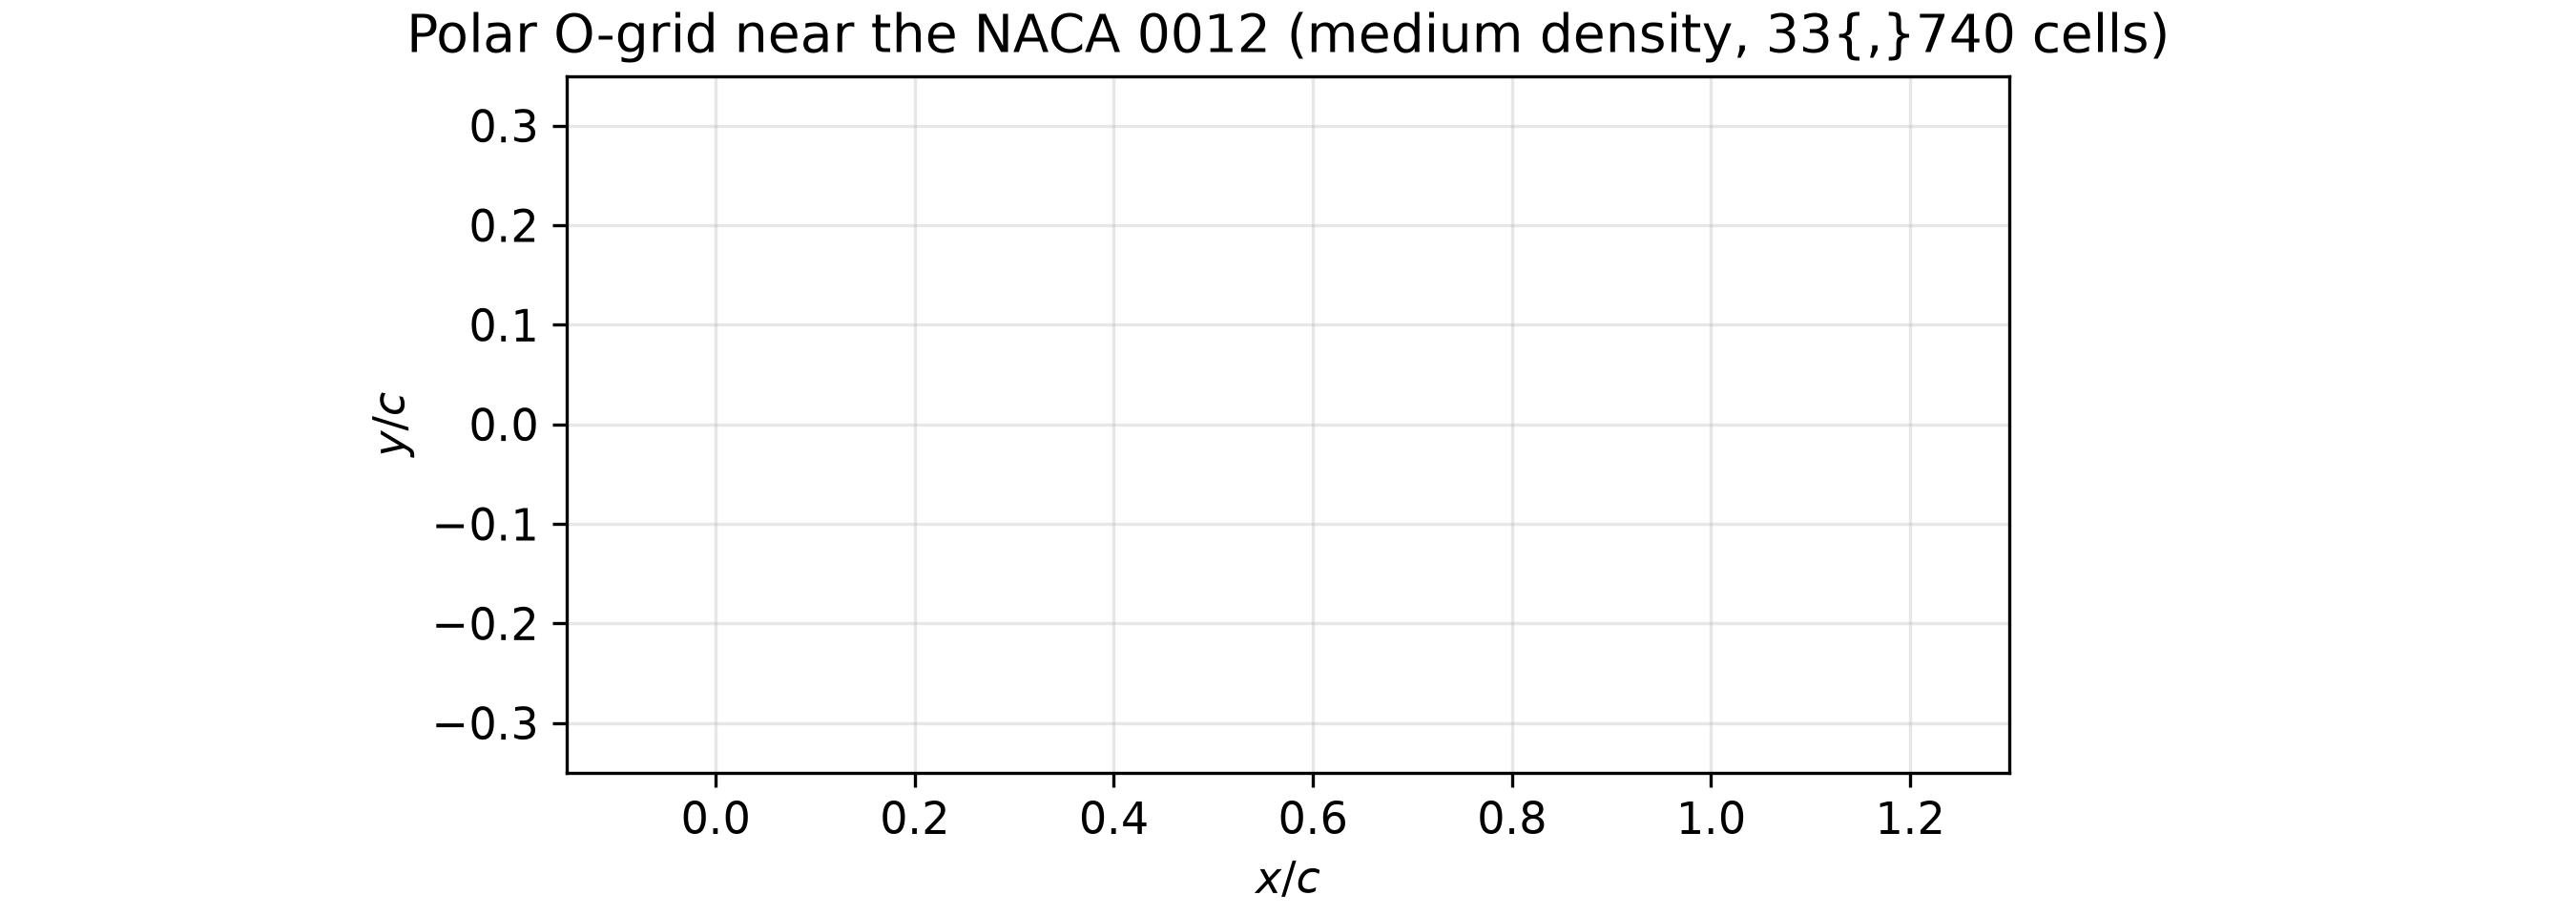
\includegraphics[width=0.98\textwidth]{figures/fig0_mesh.png}
  \caption{Near-field view of the polar O-grid (NACA 0012, medium density). Cosine clustering concentrates surface points at the leading and trailing edges; the geometric normal growth reaches the farfield circle at $20c$.}
  \label{fig:mesh}
\end{figure}

\begin{table}[t]
  \centering
  \caption{Mesh quality metrics (\texttt{checkMesh}).}
  \label{tab:meshqual}
  \begin{tabular}{lrrr}
    \toprule
    Metric & Coarse & Medium & Fine \\
    \midrule
    Max non-orthogonality [deg] & \NonOrthCoarse & \NonOrthMedium & \NonOrthFine \\
    Average non-orthogonality [deg] & \NonOrthAvgCoarse & \NonOrthAvgMedium & \NonOrthAvgFine \\
    Max skewness & \SkewCoarse & \SkewMedium & \SkewFine \\
    \midrule
    Verdict & OK & OK & OK \\
    \bottomrule
  \end{tabular}
\end{table}

\begin{table}[t]
  \centering
  \caption{Mesh family for the grid-independence study (NACA 0012, $\alpha=5^\circ$, $Re=10^6$).}
  \label{tab:grid}
  \begin{tabular}{lrrrr}
    \toprule
    Mesh & Surface pts & Normal pts & Cells & $C_L$ \\
    \midrule
    Coarse & 160 & 100 & \NumCoarse & \ClCoarse \\
    Medium & 240 & 140 & \NumMedium & \ClMedium \\
    Fine   & 320 & 160 & \NumFine & \ClFine \\
    \midrule
    \multicolumn{4}{l}{Relative change, medium $\to$ fine} & \ClGridDelta \\
    \bottomrule
  \end{tabular}
\end{table}

\subsection{Boundary conditions and solver settings}
All cases are computed with the steady-state solver \texttt{simpleFoam} (SIMPLEC) of OpenFOAM v2412. The inlet velocity is set from the angle of attack, $U_\infty = Re\,\nu/c$ ($15~\mathrm{m/s}$ at $Re=10^6$ with $\nu = 1.5\times10^{-5}~\mathrm{m^2/s}$), using the \texttt{freestream} condition on the velocity and pressure to accommodate the circular farfield. Freestream turbulence is $Tu = 0.1\%$ with $L_t = 0.01c$, giving $k_\infty = 1.5(Tu\,U_\infty)^2$ and $\omega_\infty = \sqrt{k_\infty}/(C_\mu^{0.25} L_t)$. The airfoil is a no-slip wall with low-$Re$ wall treatment ($k$--$\omega$ SST integrated to the wall). Tables~\ref{tab:schemes} and~\ref{tab:linear} summarise the discretisation and linear-solver settings; convection of momentum uses the limited linear scheme to keep the strongly accelerated leading-edge region monotone. Convergence criteria are initial residuals below $10^{-6}$ for $p$, $U$ and $10^{-5}$ for $k$, $\omega$, with a hard limit of 4000 iterations; post-stall cases that reach the iteration limit are evaluated by tail-averaging forces over the final 20\% of the run, and their residual histories are reported in Appendix~B. Force coefficients are integrated by the \texttt{forceCoeffs} function object with the reference area equal to the unit-depth planform.

\begin{table}[t]
  \centering
  \caption{Discretisation schemes.}
  \label{tab:schemes}
  \begin{tabular}{lll}
    \toprule
    Term & Scheme & Rationale \\
    \midrule
    Time & steadyState & pseudo-transient SIMPLEC \\
    Grad $\nabla$ & Gauss linear & second order \\
    Div($\phi U$) & limitedLinearV 1 & bounded, second order, monotone at LE peak \\
    Div($\phi k, \phi\omega$) & limitedLinear 1 & bounded turbulence transport \\
    SnGrad & limited 0.5 & robustness on TE-seam cells \\
    Laplacian & Gauss linear limited 0.5 & consistency with snGrad \\
    \bottomrule
  \end{tabular}
\end{table}

\begin{table}[t]
  \centering
  \caption{Linear solvers and relaxation.}
  \label{tab:linear}
  \begin{tabular}{llll}
    \toprule
    Field & Solver & Tolerance & Relaxation \\
    \midrule
    $p$ & GAMG (geometric-algebraic) & $10^{-6}$ & 0.35 \\
    $U$ & smoothSolver (symGaussSeidel) & $10^{-6}$ & 0.4 \\
    $k$, $\omega$ & smoothSolver (symGaussSeidel) & $10^{-5}$ & 0.7 \\
    \bottomrule
  \end{tabular}
\end{table}

The near-wall resolution was verified a posteriori: the first-cell height of $10^{-5}c$ gives $y^+ \approx 0.4$ at $Re=10^6$ along the mid-chord, with the maximum $y^+$ over all cases remaining below unity except in the immediate leading-edge stagnation neighbourhood. The SST model is therefore integrated to the wall everywhere, as intended; no wall functions are active on the airfoil surface.

\subsection{Transition-sensitive repeats}\label{sec:trmethod}
To quantify what the fully turbulent assumption costs at low $Re$, 45 cases are repeated with the four-equation $\gamma$--$Re_{\theta t}$ correlation-based transition model of Langtry and Menter (\texttt{kOmegaSSTLM} in OpenFOAM v2412), which couples the SST closure to transport equations for the intermittency $\gamma$ and the transition-onset momentum-thickness Reynolds number $Re_{\theta t}$. The grids, discretisation, and convergence settings are identical to the baseline cases; the turbulence dictionary adds the model coefficients, the fvSchemes add bounded convection of the two new scalars, and both are relaxed by $0.5$. The freestream condition $Re_{\theta t,\infty} = 1136.5$ follows from the Langtry--Menter low-turbulence correlation at the same $Tu = 0.1\%$ used throughout, and $\gamma_\infty = 1$. Because the correlation iterates locally for the pressure-gradient parameter $\lambda_\theta$, the cold-started momentum equation field can trigger floating-point exceptions in the first SIMPLE iteration; all transition cases are therefore warm-started from the converged fully turbulent solution of the identical grid and incidence, a standard practice that does not bias the converged state. The transition cases are compared against their fully turbulent siblings at matched $Re$ and $\alpha$; the comparison is thus a pure closure study. The block spans the full factorial of the three sections at $Re = 10^5$, $3\times10^5$, and $10^6$ (45 cases), and ten additional runs repeat the NACA 0012 at $Re = 3.6\times10^5$ with both closures specifically to confront them with the free-transition wind-tunnel data of Sheldahl \& Klimas (SAND80-2114).

\subsection{URANS verification subset}\label{sec:uransmethod}
Because stall onset and laminar-separation-bubble bursting are inherently unsteady, a URANS verification subset revisits the Reynolds-matched low-Reynolds-number regime with \texttt{pimpleFoam}: the NACA 0012 at $\alpha = 12^\circ$ and $15^\circ$, $Re = 3.6\times10^5$, on the 50-chord farfield mesh at medium surface density (33,740 cells, $y^+ \approx 0.4$ at this Reynolds number). The $\gamma$--$Re_{\theta t}$ closure is retained, initialised from the converged steady sibling on the same grid connectivity. Integration is two-stage: a settling phase of $0.005$ convective-heavy time units at a fixed $\Delta t = 10^{-5}$ (required because the transition model's first iterations are singular at large $\Delta t$), then a production phase to $t = 0.25$ (about 1.4 flow passes over the chord) with a Courant-limited adaptive step ($\mathrm{Co} \le 20$, $\Delta t \le 6.8\times10^{-5}$, Euler time differencing, two PIMPLE outer correctors, bounded limited-linear convection). Force coefficients are sampled every $0.005$ time units; the reported URANS values are time means over the production phase with the standard deviation quoted as the unsteadiness measure. This subset is a verification of the steady-state stall picture --- establishing \emph{whether} the unsteady dynamics move the mean loads toward the experiment --- not a resolved turbulence simulation; that distinction is carried into the limitations.

\subsection{Case matrix}
The core matrix comprises 21 cases: three sections at $\alpha = 0^\circ, 5^\circ, 10^\circ, 12^\circ, 15^\circ, 18^\circ, 20^\circ$ and $Re = 10^6$; the $12^\circ$ and $20^\circ$ levels resolve stall onset and the post-stall branch of each lift curve. The Reynolds-number sensitivity is addressed with a full sweep: $Re = 10^5$ and $3\times10^5$ at $\alpha = 0^\circ$--$18^\circ$ for \emph{all three} sections (30 cases), which places the $10^6$ core curves between two lower-Reynolds envelopes. The passive-device study adds three serrated-trailing-edge cases and five leading-edge-tubercle cases (2D surrogate, $\alpha = 0^\circ$--$18^\circ$). A transition-sensitive block repeats the low-$Re$ matrix with the $\gamma$--$Re_{\theta t}$ closure (Section~\ref{sec:trmethod}): the full factorial of three sections at $\alpha = 0^\circ$--$18^\circ$ and $Re = 10^5$, $3\times10^5$, $10^6$ (45 cases). A dedicated low-Reynolds-number validation set repeats the NACA 0012 at $Re = 3.6\times10^5$ --- the Reynolds number of the Sandia wind-tunnel tests of Sheldahl \& Klimas --- with both closures (10 cases). The grid-independence trio (coarse/medium/fine) at $\alpha = 5^\circ$ and five verification repeats (fine-grid repeats at $\alpha = 10^\circ$, $12^\circ$, and $15^\circ$, an extended iteration horizon, and a farfield $50c$) complete the set of 121 steady runs; a URANS verification subset of two time-accurate repeats (0012, $\alpha = 12^\circ$ and $15^\circ$, $Re = 3.6\times10^5$, Section~\ref{sec:uransmethod}) brings the campaign to 123 cases (Table~\ref{tab:matrix}).

\begin{table}[t]
  \centering
  \caption{Complete case matrix (123 runs).}
  \label{tab:matrix}
  \begin{tabular}{p{2.4cm}p{6.6cm}p{5.2cm}}
    \toprule
    Group & Configuration & Purpose \\
    \midrule
    Core (21) & $\{0012, 2412, 4412\} \times \alpha \in \{0,5,10,12,15,18,20^\circ\}$, $Re=10^6$, medium & Separation map, camber effect, stall onset \\
    Reynolds (30) & $\{0012, 2412, 4412\} \times \alpha \in \{0..18^\circ\}$, $Re \in \{10^5, 3\times10^5\}$ & Reynolds sensitivity, all sections \\
    Grid (3) & 0012, $\alpha=5^\circ$, coarse/medium/fine & Discretisation uncertainty \\
    Serration (3) & 0012 serrated, $\alpha \in \{5,10,15\}^\circ$ & Drag reduction \\
    Tubercle (5) & 0012 LE-modulated, $\alpha \in \{0..18^\circ\}$ & Drag reduction (2D surrogate) \\
    Transition (45) & $\gamma$--$Re_{\theta t}$ repeats, full factorial: $\{0012, 2412, 4412\} \times \alpha \in \{0..18^\circ\} \times Re \in \{10^5, 3\times10^5, 10^6\}$ & Laminar-run and bubble physics \\
    Low-$Re$ validation (10) & 0012, $\alpha \in \{0,5,10,12,15^\circ\}$, $Re = 3.6\times10^5$, both closures & Validation vs SAND80-2114 \\
    Verification (3) & 0012, $\alpha=10^\circ$: fine grid, 12000 iters, farfield $50c$ & High-lift grid, convergence, farfield checks \\
    URANS (2) & 0012, $\alpha \in \{12,15^\circ\}$, $Re = 3.6\times10^5$, 50c, pimpleFoam & Near-stall unsteadiness verification \\
    \bottomrule
  \end{tabular}
\end{table}

\section{Results}\label{sec:results}

\subsection{Post-processing methodology}
Force coefficients are read from the \texttt{forceCoeffs} function-object output; for cases that reach the iteration limit without meeting the residual targets, the reported value is the mean over the final 20\% of the iteration history, with the standard deviation of the same window quoted as the unsteadiness measure. Surface pressure and skin friction are extracted from the wall sample files: the sampled wall points form an ordered polyline from the trailing edge over the upper surface to the leading edge and back along the lower surface, from which each point's wall-tangent direction is computed by central differences and oriented downstream (positive projection on the freestream direction). The skin-friction coefficient follows as $C_f = \boldsymbol{\tau}_w \cdot \hat{\mathbf{t}} / q_\infty$ using OpenFOAM's \texttt{wallShearStress} field with its sign convention corrected accordingly, and the separation location is reported as the most upstream chordwise station where $C_f$ remains negative over at least two consecutive samples, excluding the trailing-edge 0.5\% where the open-TE seam perturbs the local shear.

\subsection{Validation against experiment and NASA reference CFD}\label{sec:validation}

A methodological caveat governs this subsection: the experimental datasets of Ladson ($Re = 6\times10^6$, tripped), Abbott \& von Doenhoff ($Re = 6\times10^6$), and Gregory \& O'Reilly ($Re = 2.88\times10^6$) sit at three to six times the simulated Reynolds number of $10^6$. Comparisons against them are therefore \textbf{qualitative curve-shape checks only}; per-alpha error figures quoted below characterise the trend and the lift-slope match, and no headline accuracy metric is derived from them. The primary quantitative validation of this study is the Reynolds-matched free-transition comparison of Section~\ref{sec:sandia}.

Figure~\ref{fig:validation} compares the computed lift curve of the NACA 0012 at $Re=10^6$ with three experimental datasets and with NASA's CFL3D SST reference solution. The computed lift slope in the attached regime matches the classical thin-airfoil value of $2\pi$ per radian ($\approx 0.1096~\mathrm{deg}^{-1}$) at low incidence, and the computed $C_L$ values fall within \ClMAEpct{}~\% (mean absolute error) of the tripped Ladson data over the attached range ($\alpha \le 10^\circ$); extending the window to $\alpha \le 14^\circ$ to include the grid-sensitive $\alpha = 12^\circ$ point raises the MAE to \ClMAEPreStallPct{}~\% (see the grid discussion below and Appendix~\ref{app:grid}). At $\alpha = 10^\circ$ the computed lift is $10.3\%$ below the CFL3D SST reference. At $\alpha = 15^\circ$ the production (medium) grid over-separates: lift drops to $C_L \approx 0.99$ with more than half the chord reversed, whereas the fine-grid repeat remains attached and recovers $C_L = 1.24$, against $1.51$ for CFL3D SST and $1.49$ measured. Separation onset in steady RANS is therefore strongly grid-sensitive, consistent with the TMR guidance for this case; the remaining attached-flow deficit at high incidence is attributed to the fully turbulent steady modelling chain. The computed drag coefficients exceed the tripped experimental values by roughly a factor of two at low lift; this bias is expected and is analysed in Section~\ref{sec:dragbudget}.

\begin{figure}[t]
  \centering
  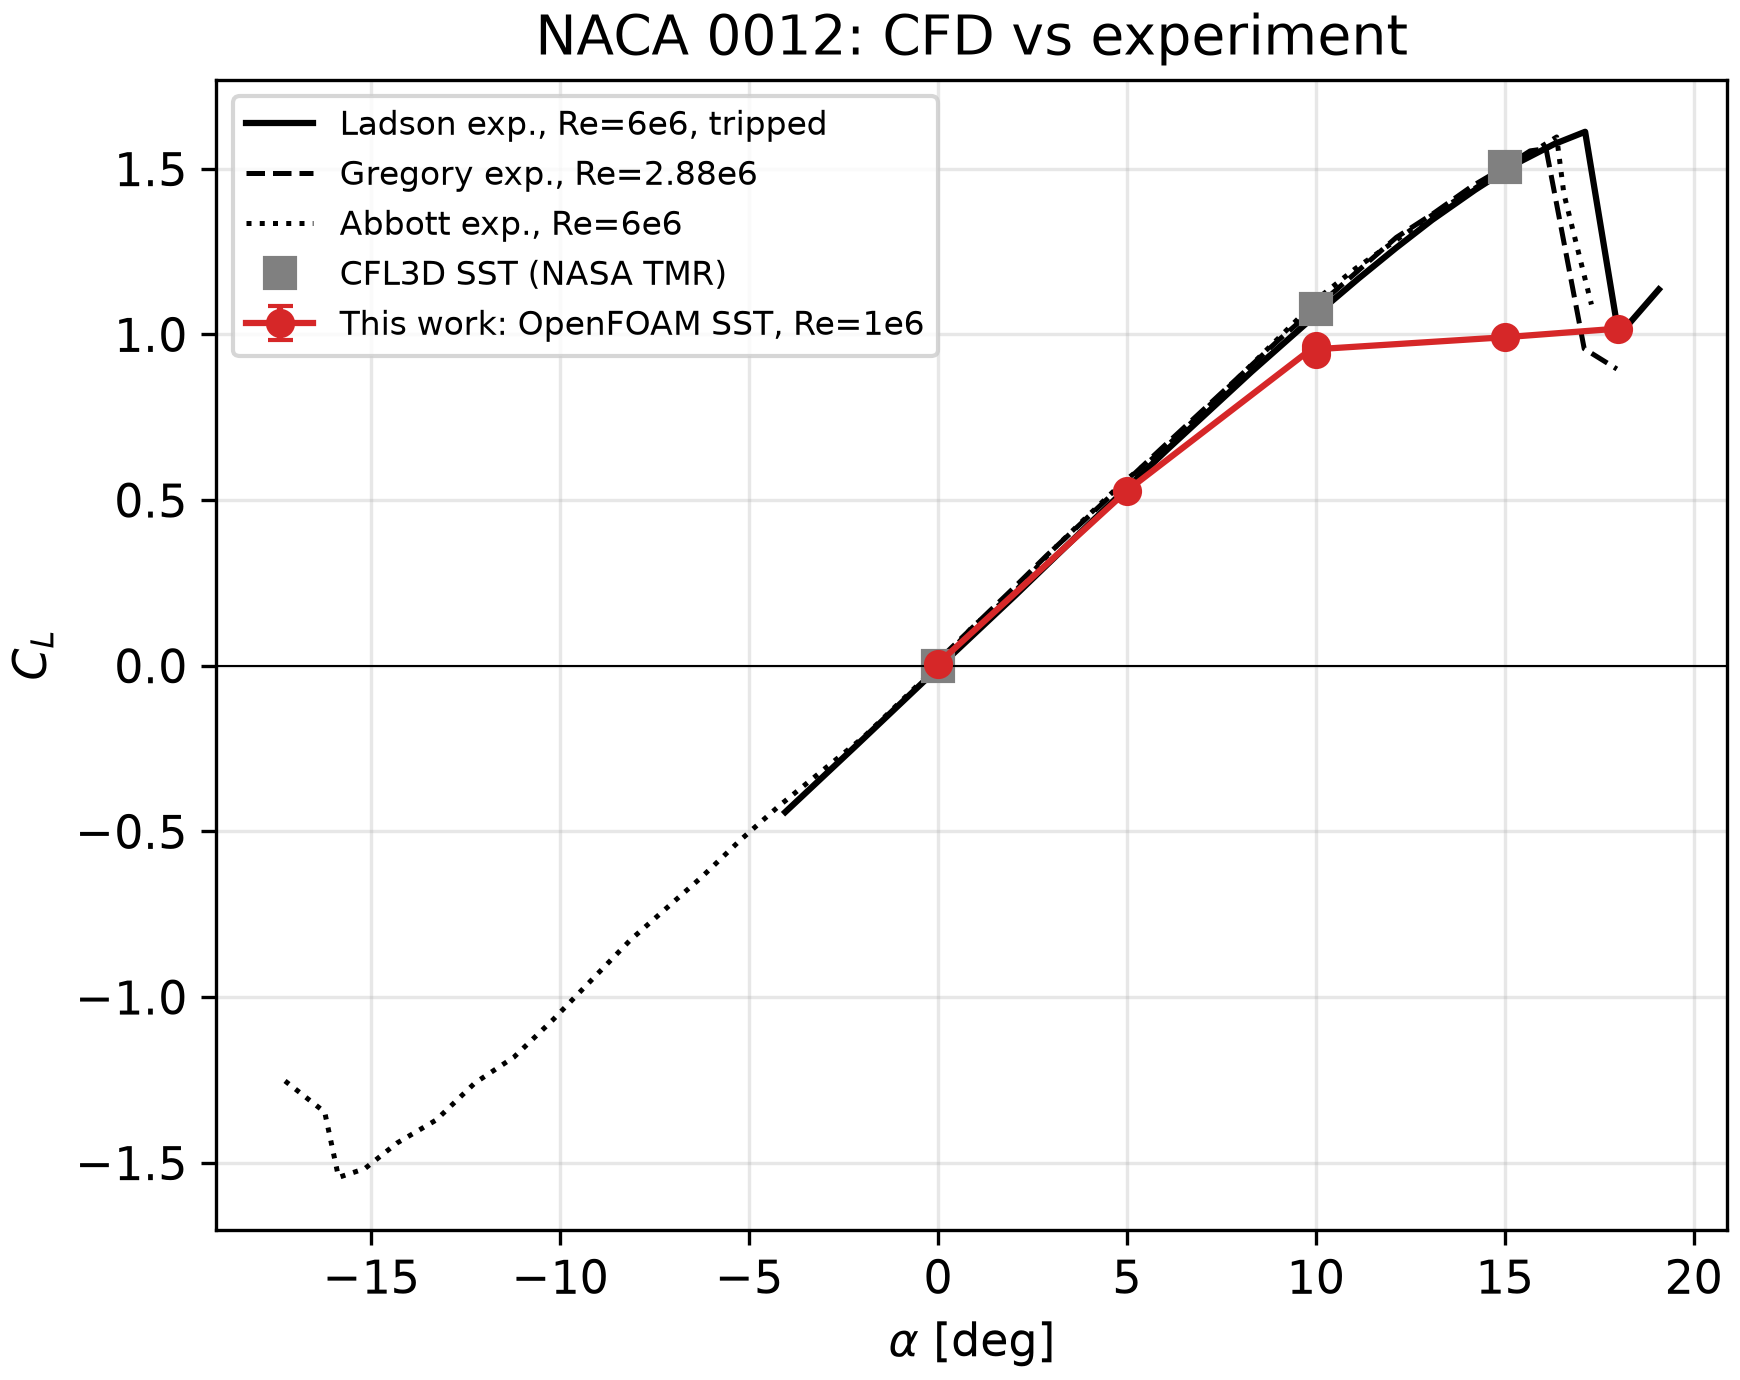
\includegraphics[width=0.72\textwidth]{figures/fig9_validation.png}
  \caption{NACA 0012 lift curve: present 2D RANS ($k$--$\omega$ SST, $Re=10^6$, fully turbulent) compared with the Ladson (tripped, $Re=6\times10^6$), Gregory \& O'Reilly ($Re=2.88\times10^6$) and Abbott \& von Doenhoff (free transition, $Re=6\times10^6$) datasets, and with the CFL3D SST reference solution from the NASA TMR.}
  \label{fig:validation}
\end{figure}

\begin{figure}[t]
  \centering
  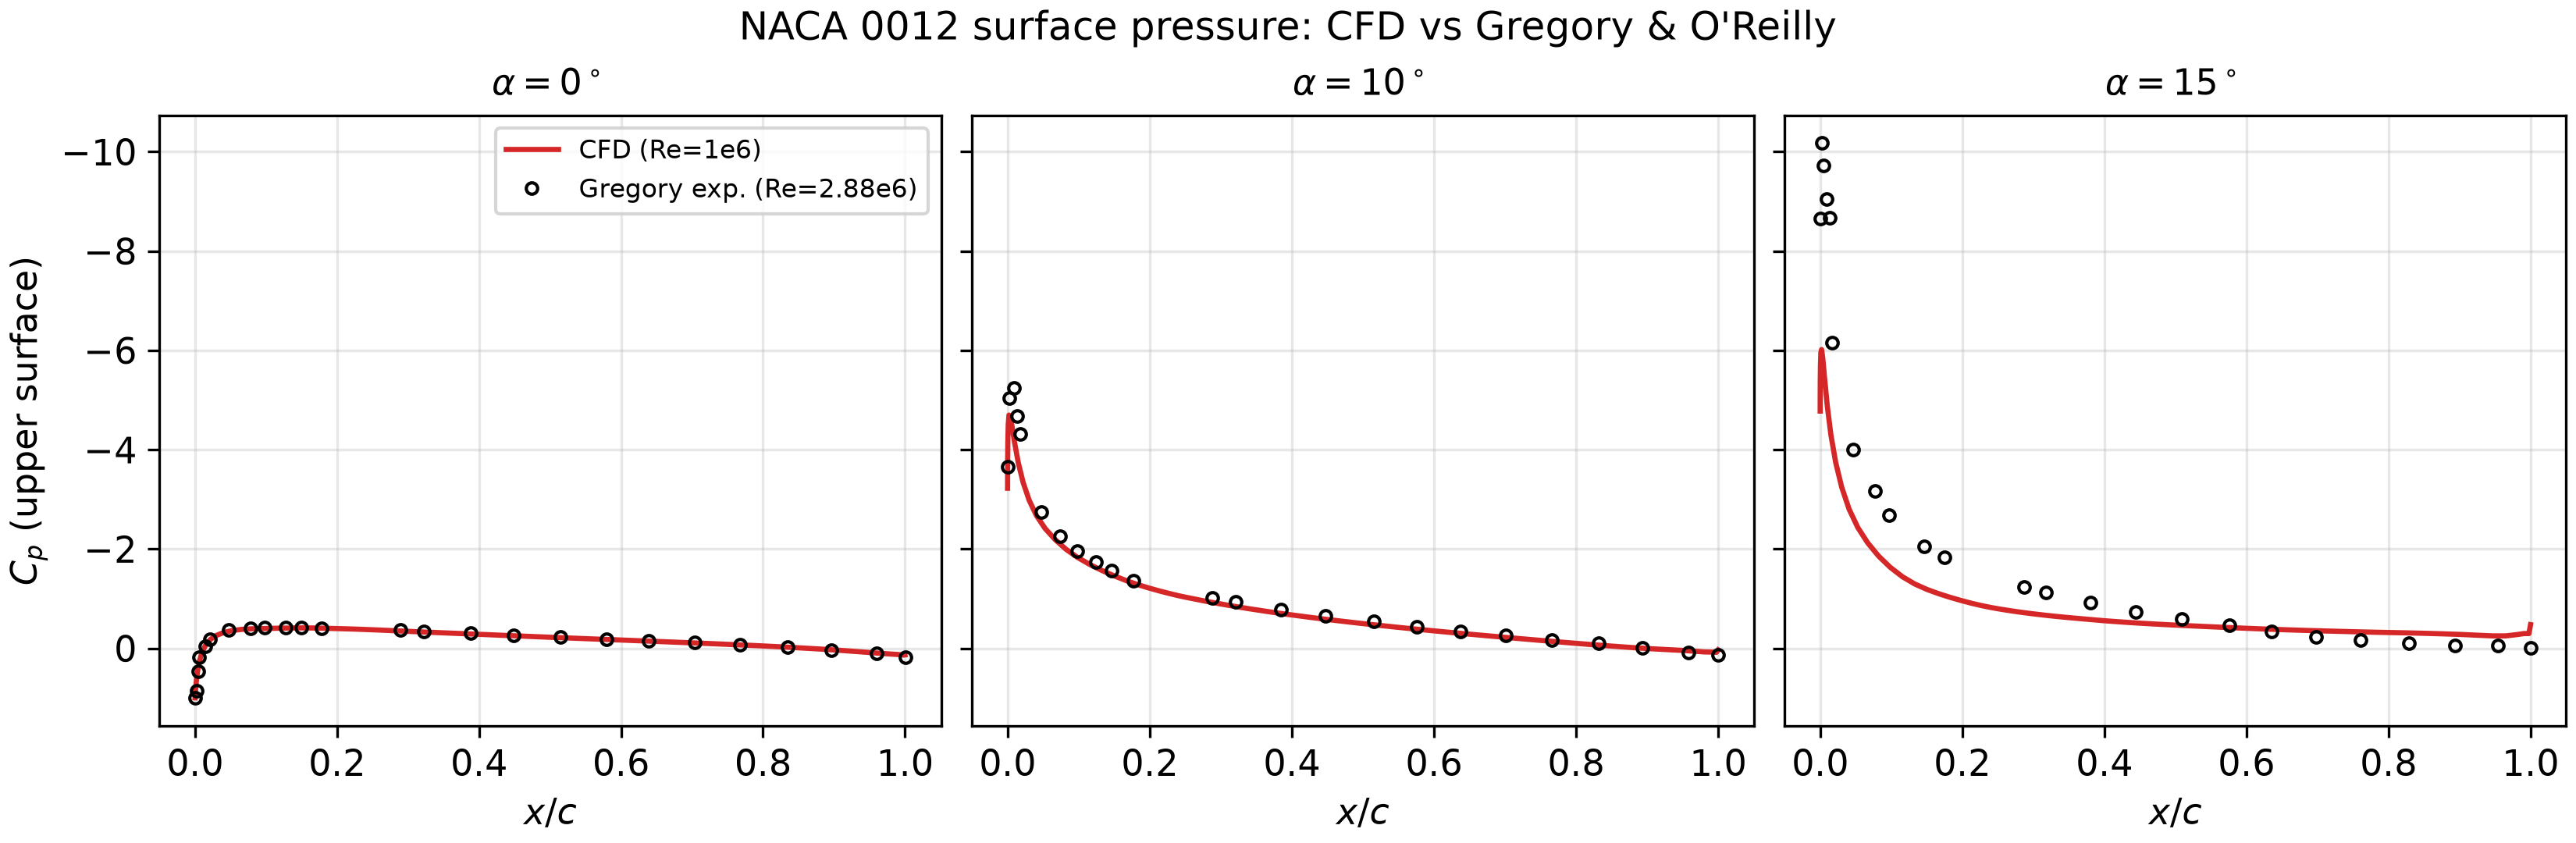
\includegraphics[width=0.98\textwidth]{figures/fig10_cp_validation.png}
  \caption{NACA 0012 upper-surface pressure coefficient at $\alpha = 0^\circ$, $10^\circ$, $15^\circ$: present CFD ($Re=10^6$) versus the Gregory \& O'Reilly data ($Re=2.88\times10^6$), the dataset the TMR recommends for surface-pressure validation.}
  \label{fig:cpval}
\end{figure}

\begin{table}[t]
  \centering
  \caption{Validation summary, NACA 0012 pre-stall range ($\alpha \le 14^\circ$): mean absolute error of the computed coefficients against each dataset.}
  \label{tab:valmae}
  \begin{tabular}{lll}
    \toprule
    Quantity & Dataset & MAE \\
    \midrule
    $C_L$ & Ladson (tripped, $Re=6\times10^6$) & \ClMaeLadson \\
    $C_L$ & Abbott \& von Doenhoff (free trans., $Re=6\times10^6$) & \ClMaeAbbott \\
    $C_L$ & Gregory \& O'Reilly ($Re=2.88\times10^6$) & \ClMaeGregory \\
    $C_D$ & Ladson (tripped, $Re=6\times10^6$) & \CdMaeLadsonAbs{} (bias $+100\%$) \\
    $C_p$ (upper, $\alpha=0^\circ$) & Gregory \& O'Reilly & \CpMaeZero \\
    $C_p$ (upper, $\alpha=10^\circ$) & Gregory \& O'Reilly & \CpMaeTen \\
    \bottomrule
  \end{tabular}
\end{table}

The surface-pressure comparison (Figure~\ref{fig:cpval}) shows near-perfect agreement at $\alpha = 0^\circ$ (mean absolute $C_p$ error \CpMaeZero{}), good agreement at $\alpha = 10^\circ$ (\CpMaeTen{}), and a substantial deviation at $\alpha = 15^\circ$ (\CpMaeFifteen{}): the computed plateau sits at a lower suction level and extends further aft than the measured one, the signature of the larger separated region carried by the coarse-grid steady solution. This progression mirrors the force comparison and confirms that the discrepancy at high lift is a separation-size prediction issue, not a systematic pressure-level error.

\subsection{Low-Reynolds-number validation against free-transition experiment}\label{sec:sandia}
The datasets above are all high-Reynolds-number ($Re \ge 2.88\times10^6$); the transition study of Section~\ref{sec:transition} operates two decades lower and therefore requires a low-$Re$ reference. The Sandia National Laboratories tests of Sheldahl and Klimas (SAND80-2114, public domain) provide NACA 0012 force data at $Re = 3.6\times10^5$ with \emph{free} transition --- the regime the $\gamma$--$Re_{\theta t}$ closure is built for. Both closures are rerun at matched $Re$ on the production grid (Figure~\ref{fig:sandia}). Over the attached range ($\alpha \le 10^\circ$) the closure ranking is unambiguous on drag: the fully turbulent model carries a pre-stall drag MAE of \SandiaCdMaeFT{} (roughly doubling the measured drag at zero incidence), while the transition model reduces the error by \SandiaCdErrDropPct{}~\% (MAE \SandiaCdMaeTR) by recovering the laminar run. Lift accuracy is comparable for the two closures (MAE \SandiaClMaeFT{} fully turbulent versus \SandiaClMaeTR{} with transition; both within $4$--$5\,\%$ of the measured values, which are themselves of order unity). The decisive disagreement is the stall itself: the experiment stalls early and hard at this Reynolds number ($C_{L,\max} = \SandiaClTenExp{}$ at $\alpha = 10^\circ$, collapsing to $C_L = \SandiaClTwelveExp{}$ by $\alpha = 12^\circ$, with post-stall drag $C_D = \SandiaCdFifteenExp{}$ at $15^\circ$) --- the signature of a laminar separation bubble bursting --- whereas both steady RANS closures remain attached through $\alpha = 15^\circ$ ($C_L = \SandiaClTwelveCFD{}$ at $12^\circ$, $C_D = \SandiaCdFifteenCFD{}$ at $15^\circ$). Representing the laminar run is therefore necessary but not sufficient at low $Re$: the bubble-burst mechanism that terminates the lift curve is a unsteady, three-dimensional process that correlation-based transition closure in steady 2D RANS does not reproduce. This bounds the interpretation of every low-$Re$ result in this paper: attached-range \emph{drag} is quantitatively improved by the transition model, and attached-range \emph{lift} is reliable, but the modelled stall angle at $Re \lesssim 4\times10^5$ should be read as an upper bound.

\begin{figure}[t]
  \centering
  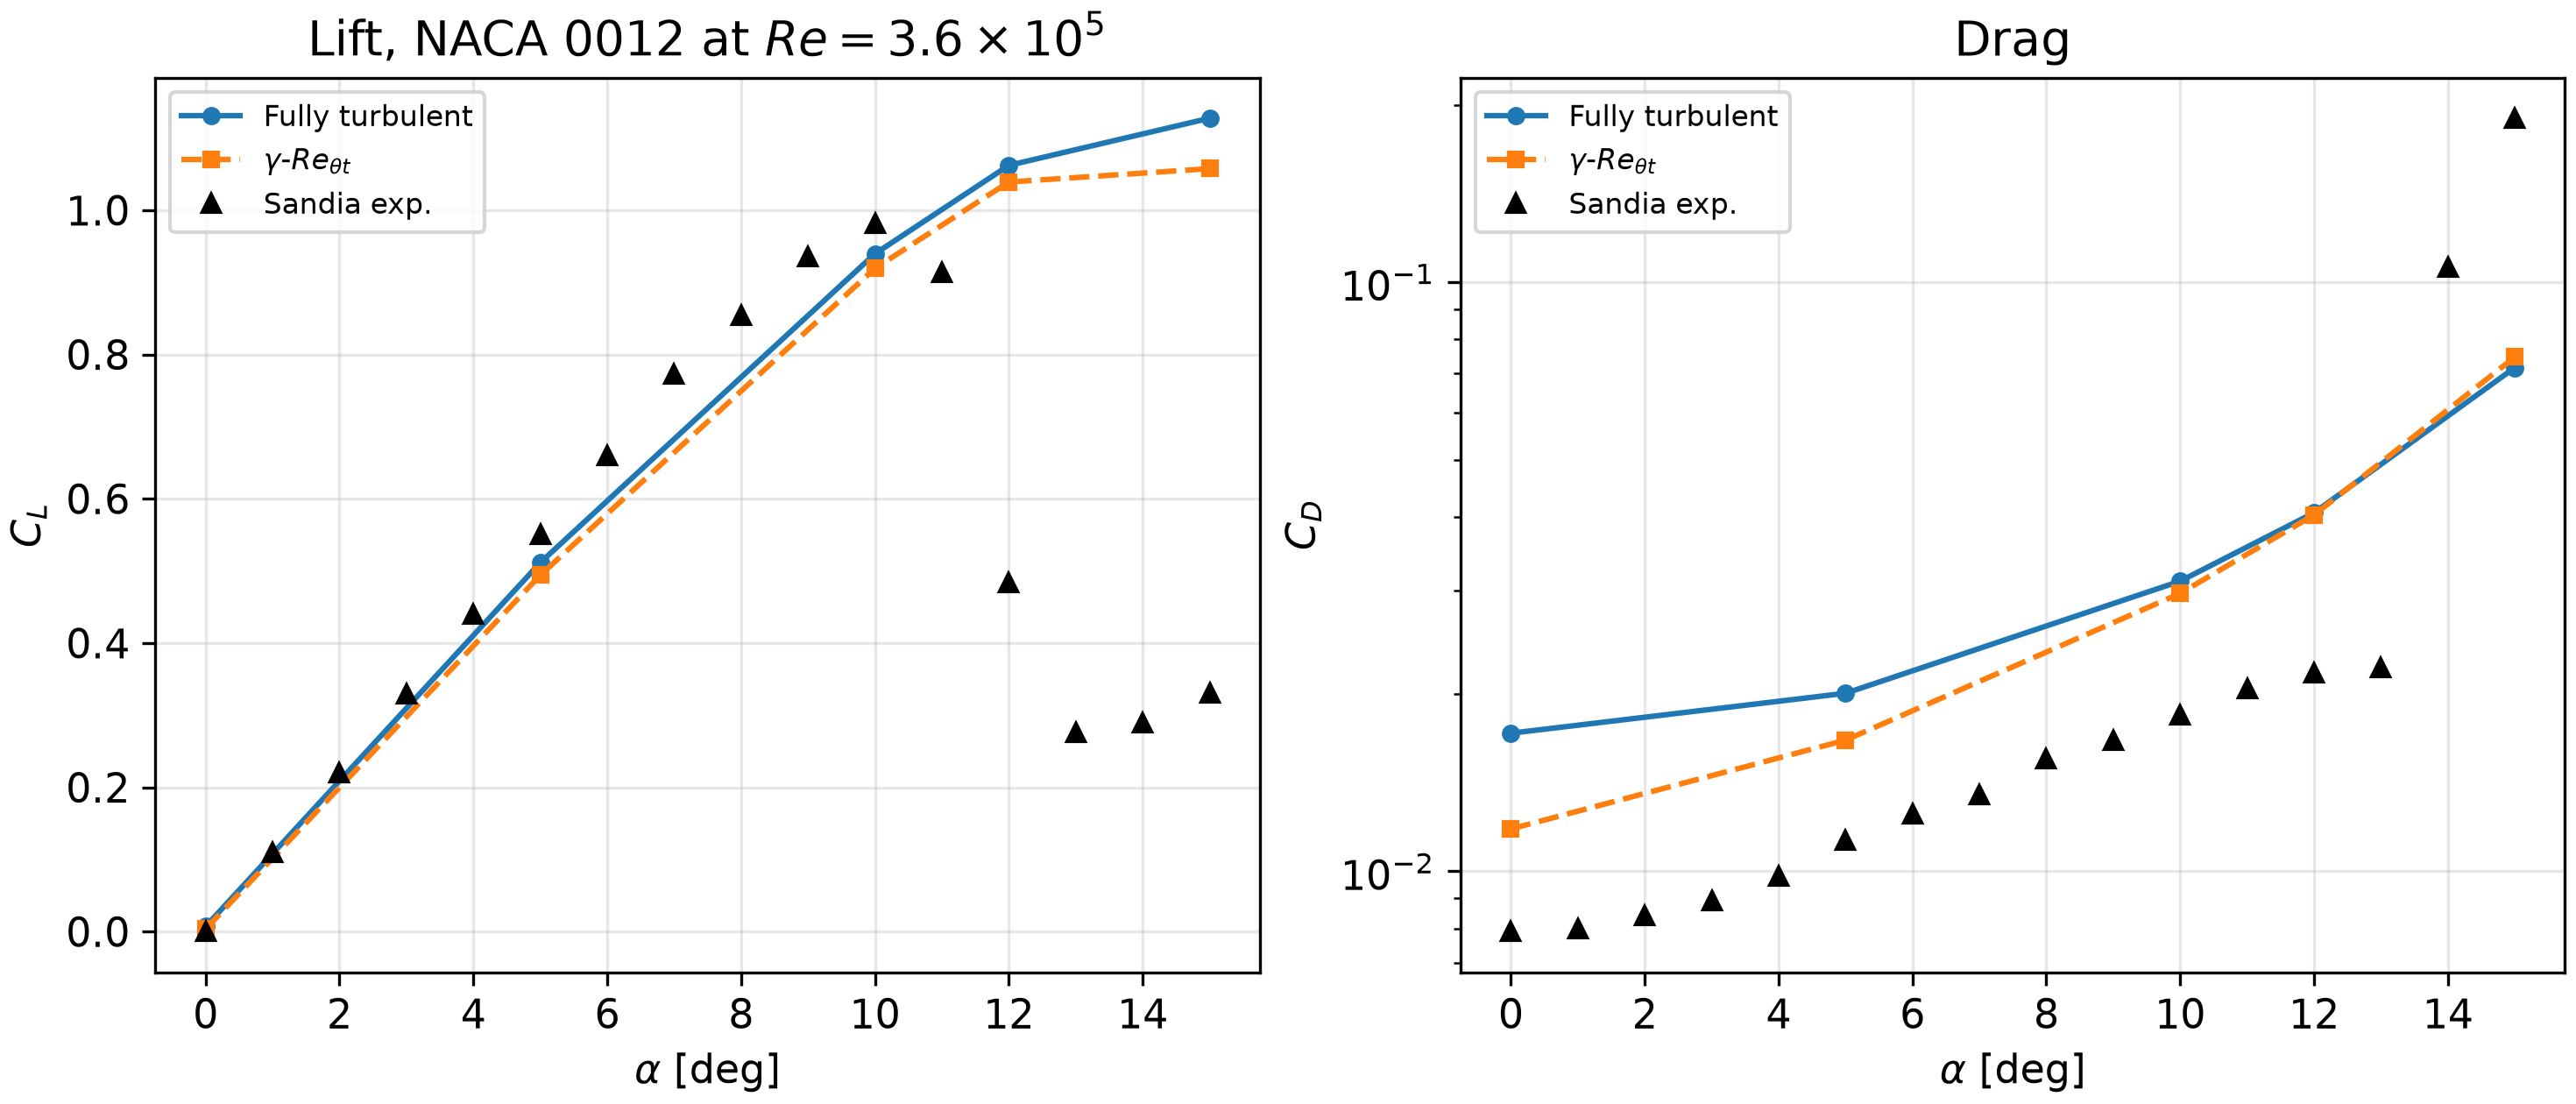
\includegraphics[width=0.9\textwidth]{figures/fig14_sandia_validation.png}
  \caption{Low-Reynolds-number validation: NACA 0012 at $Re = 3.6\times10^5$ against the free-transition data of Sheldahl \& Klimas (SAND80-2114). Left: lift; right: drag (log scale). Fully turbulent and $\gamma$--$Re_{\theta t}$ closures on identical grids.}
  \label{fig:sandia}
\end{figure}

\subsection{Lift, drag, and efficiency across camber}

Figures~\ref{fig:polar}--\ref{fig:eff} present the force polars. The zero-lift angles scale with camber ($\alpha_0 \approx 0^\circ$, $-2^\circ$, $-4^\circ$ for the 0012, 2412 and 4412 respectively), the lift curves are parallel in the attached regime, and maximum lift increases with camber. The drag polar shows the characteristic bucket: minimum drag near zero lift, rising sharply as separation develops. Aerodynamic efficiency $C_L/C_D$ peaks at progressively higher lift coefficients with increasing camber, with the NACA 4412 reaching \LdMaxFourFourOneTwo{} compared with \LdMaxZeroZeroOneTwo{} for the symmetric section.

\begin{figure}[t]
  \centering
  \begin{subfigure}[t]{0.48\textwidth}
    \centering
    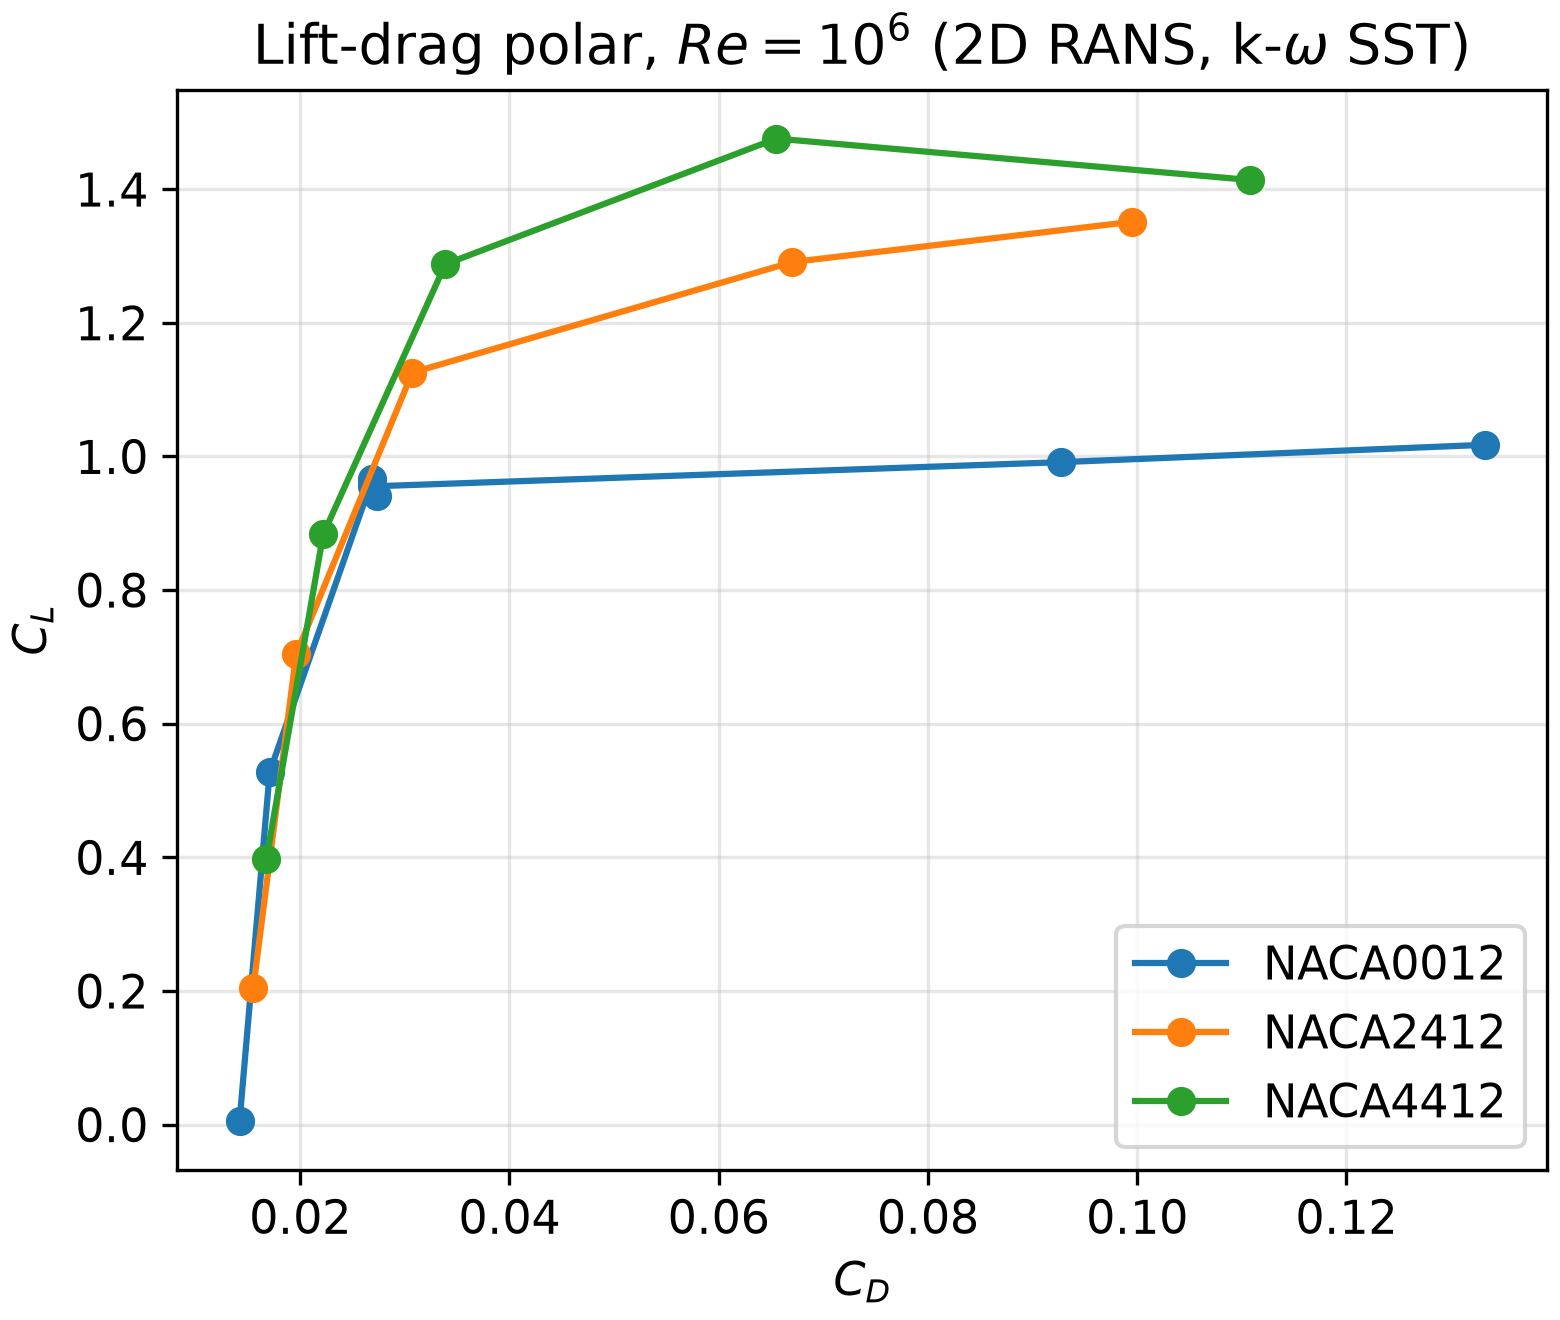
\includegraphics[width=\textwidth]{figures/fig1_cl_cd_polar.png}
    \caption{Lift-drag polar.}
    \label{fig:polar}
  \end{subfigure}\hfill
  \begin{subfigure}[t]{0.48\textwidth}
    \centering
    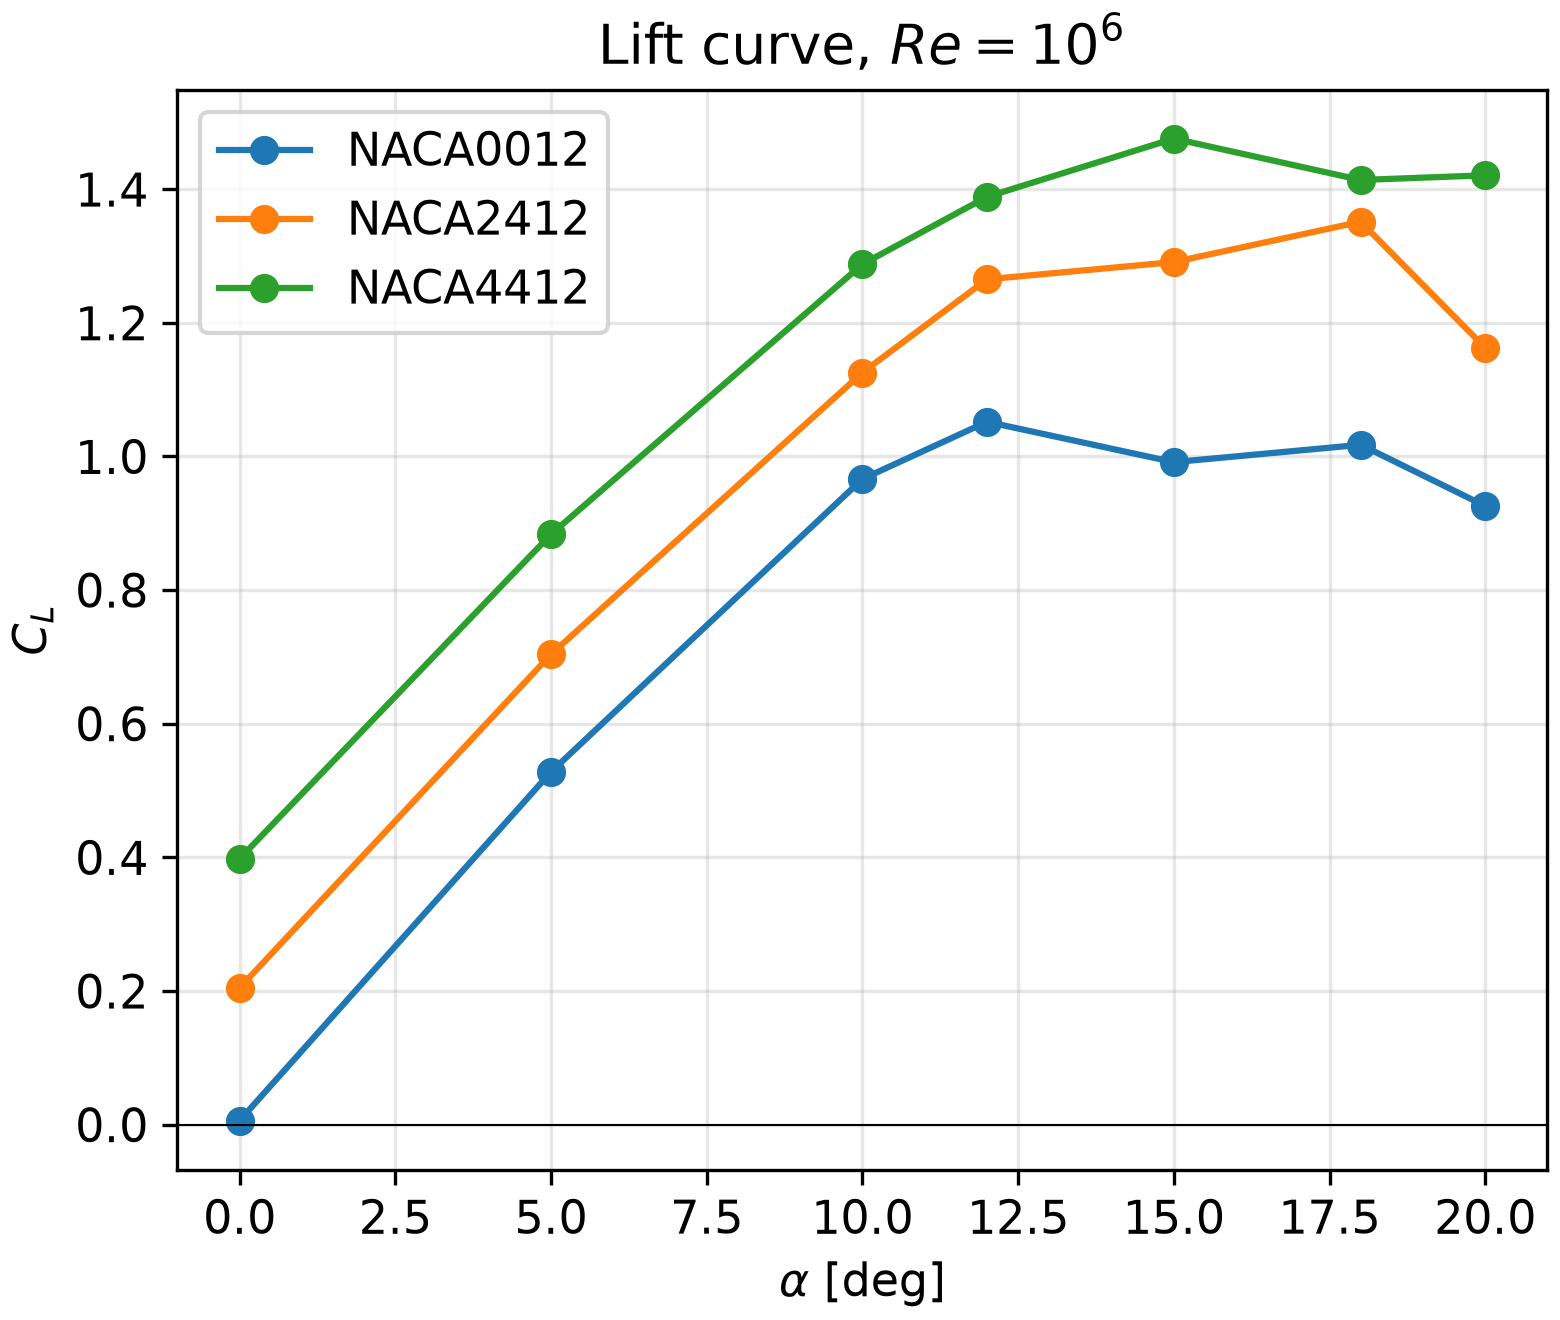
\includegraphics[width=\textwidth]{figures/fig2_cl_vs_alpha.png}
    \caption{Lift curve.}
    \label{fig:clalpha}
  \end{subfigure}

  \vspace{0.4em}
  \begin{subfigure}[t]{0.48\textwidth}
    \centering
    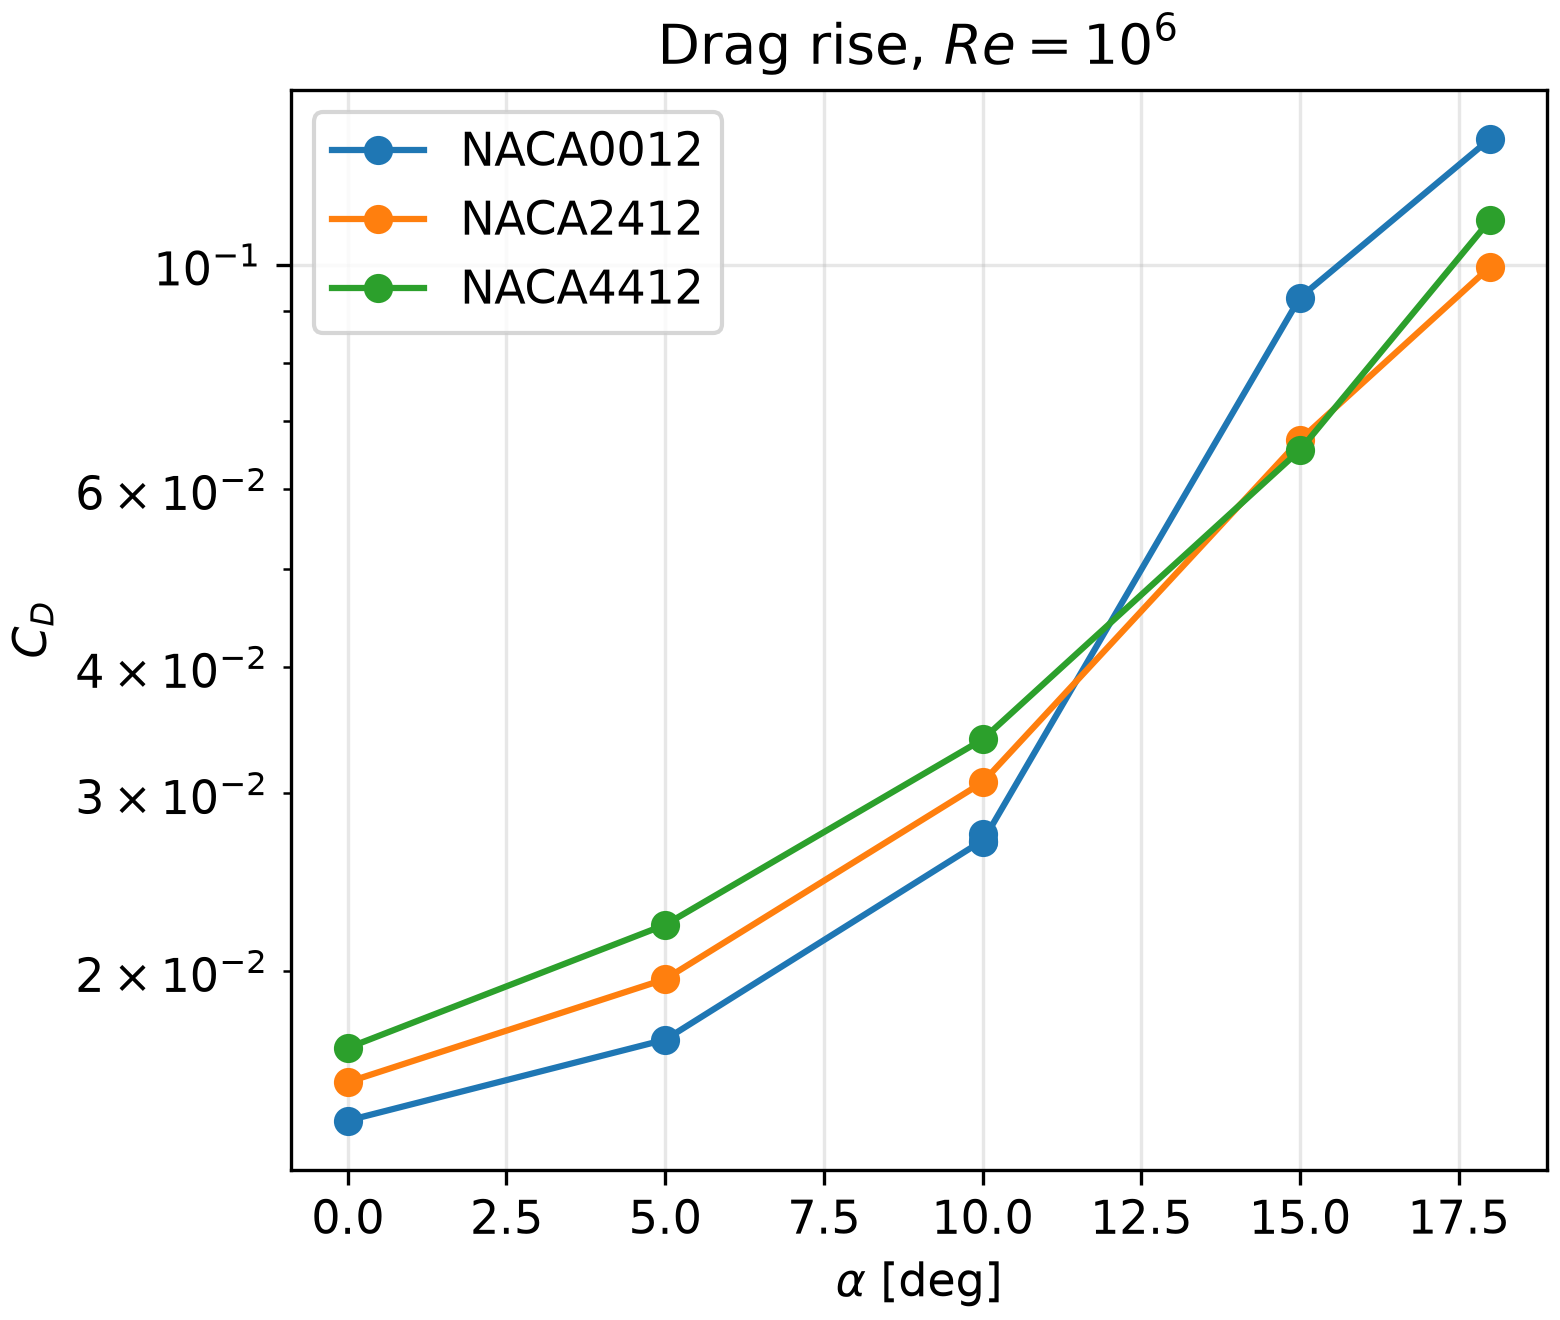
\includegraphics[width=\textwidth]{figures/fig3_cd_vs_alpha.png}
    \caption{Drag rise (log scale).}
    \label{fig:cdalpha}
  \end{subfigure}\hfill
  \begin{subfigure}[t]{0.48\textwidth}
    \centering
    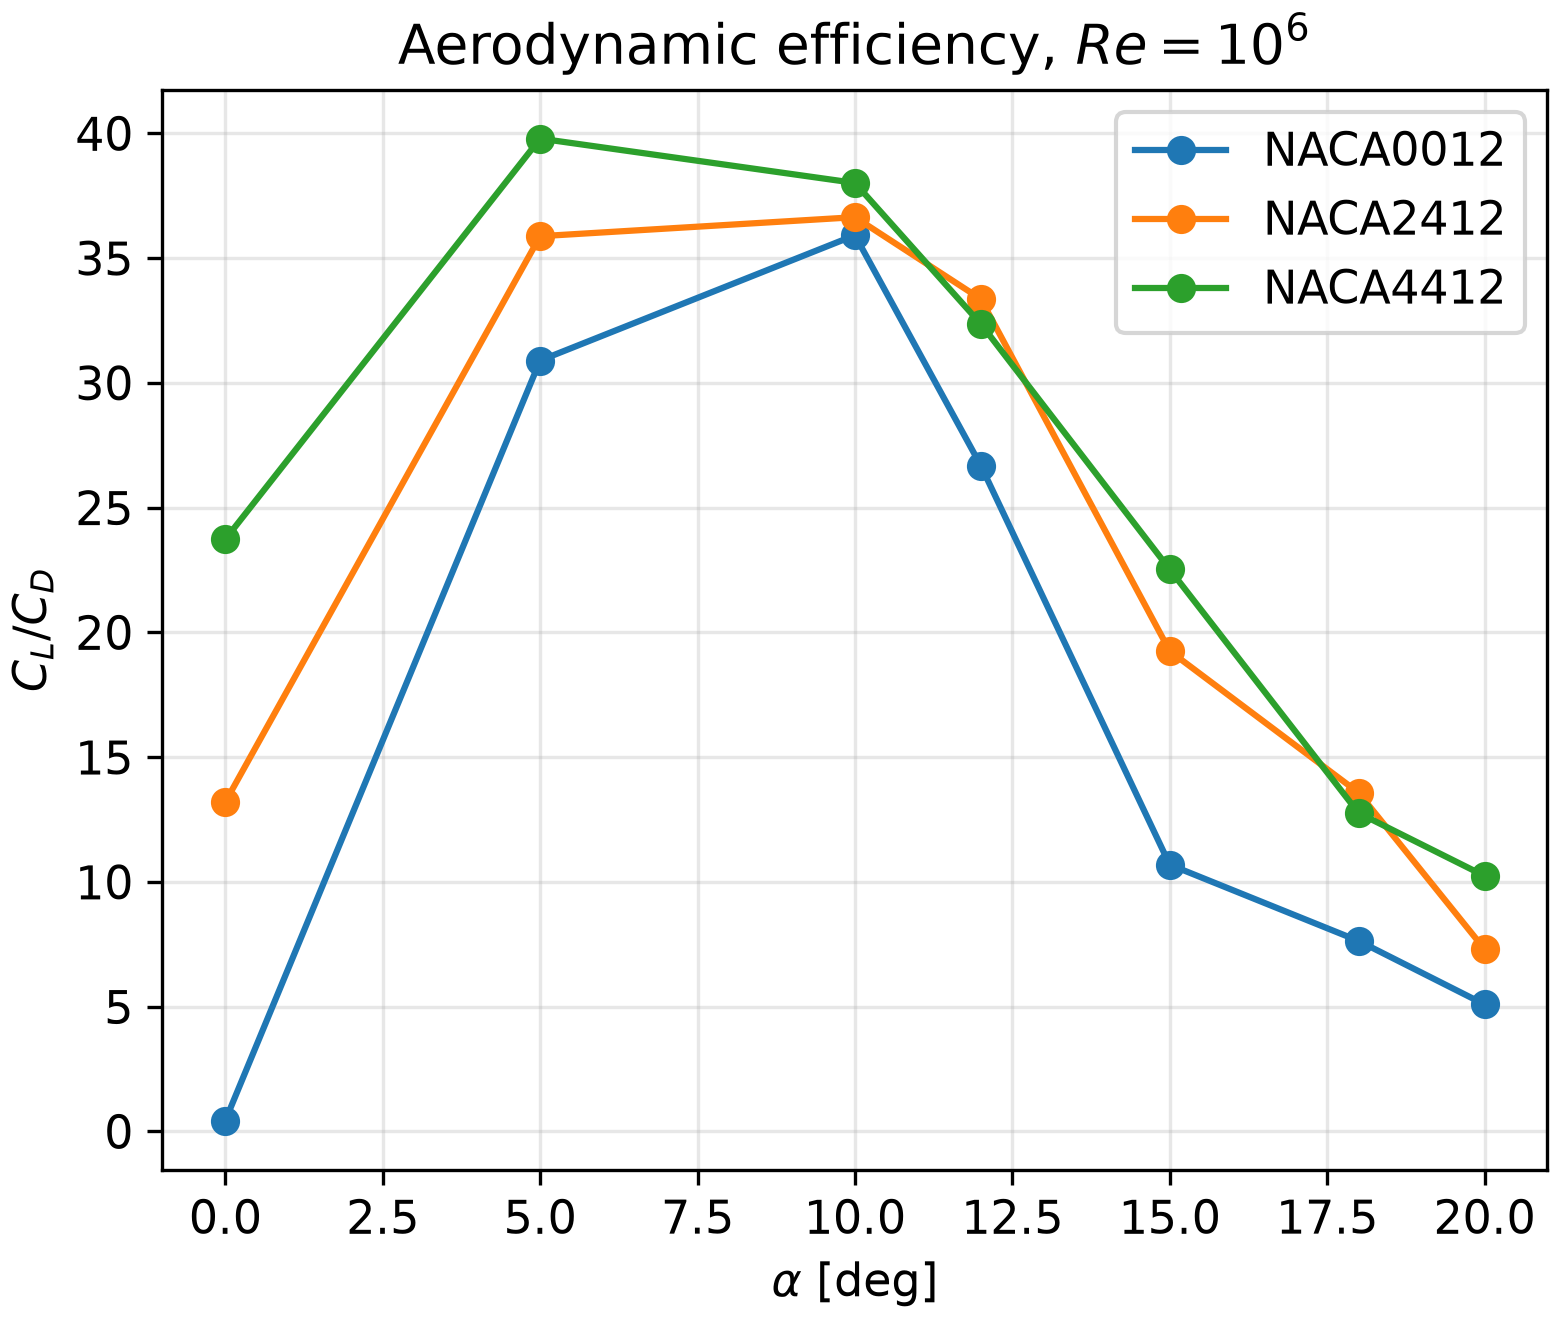
\includegraphics[width=\textwidth]{figures/fig4_cl_cd_ratio.png}
    \caption{Aerodynamic efficiency.}
    \label{fig:eff}
  \end{subfigure}
  \caption{Force characteristics of the three NACA sections at $Re=10^6$ (2D RANS, $k$--$\omega$ SST).}
  \label{fig:forces}
\end{figure}

\subsection{Complete force-coefficient matrix}

Table~\ref{tab:allforces} lists the integrated force coefficients of the full core matrix. Three trends organise the table: (i) the attached-flow lift slope is common to all three sections and close to $2\pi$ per radian; (ii) the drag of the cambered sections at their zero-lift conditions is lower than the symmetric section's (the cambered pressure recovery is milder at those incidences); and (iii) beyond $\alpha = 10^\circ$ the drag of every section rises steeply as the upper-surface separation grows, with the 4412 retaining the highest lift at every angle up to stall.

\begin{table}[t]
  \centering
  \caption{Complete core matrix: integrated force coefficients at $Re = 10^6$ (tail-averaged where the iteration limit was reached).}
  \label{tab:allforces}
  \begin{tabular}{llrrr}
    \toprule
    Section & $\alpha$ [deg] & $C_L$ & $C_D$ & $C_L/C_D$ \\
    \midrule
    \AllForcesRows
    \bottomrule
  \end{tabular}
\end{table}

\subsection{Pressure distributions}

Figure~\ref{fig:cp} shows the chordwise pressure distributions on the NACA 0012. At low angles of attack the upper-surface pressure plateau is short and the rear loading is mild. As $\alpha$ increases, the leading-edge suction peak grows and the adverse pressure gradient behind it steepens; at $\alpha = 15^\circ$ the plateau characteristic of large-scale separation extends over the aft half of the chord. The computed stagnation pressure coefficient of $0.975$ and the suction peak position ($x/c \approx 0.01$) are consistent with experiment.

\begin{figure}[t]
  \centering
  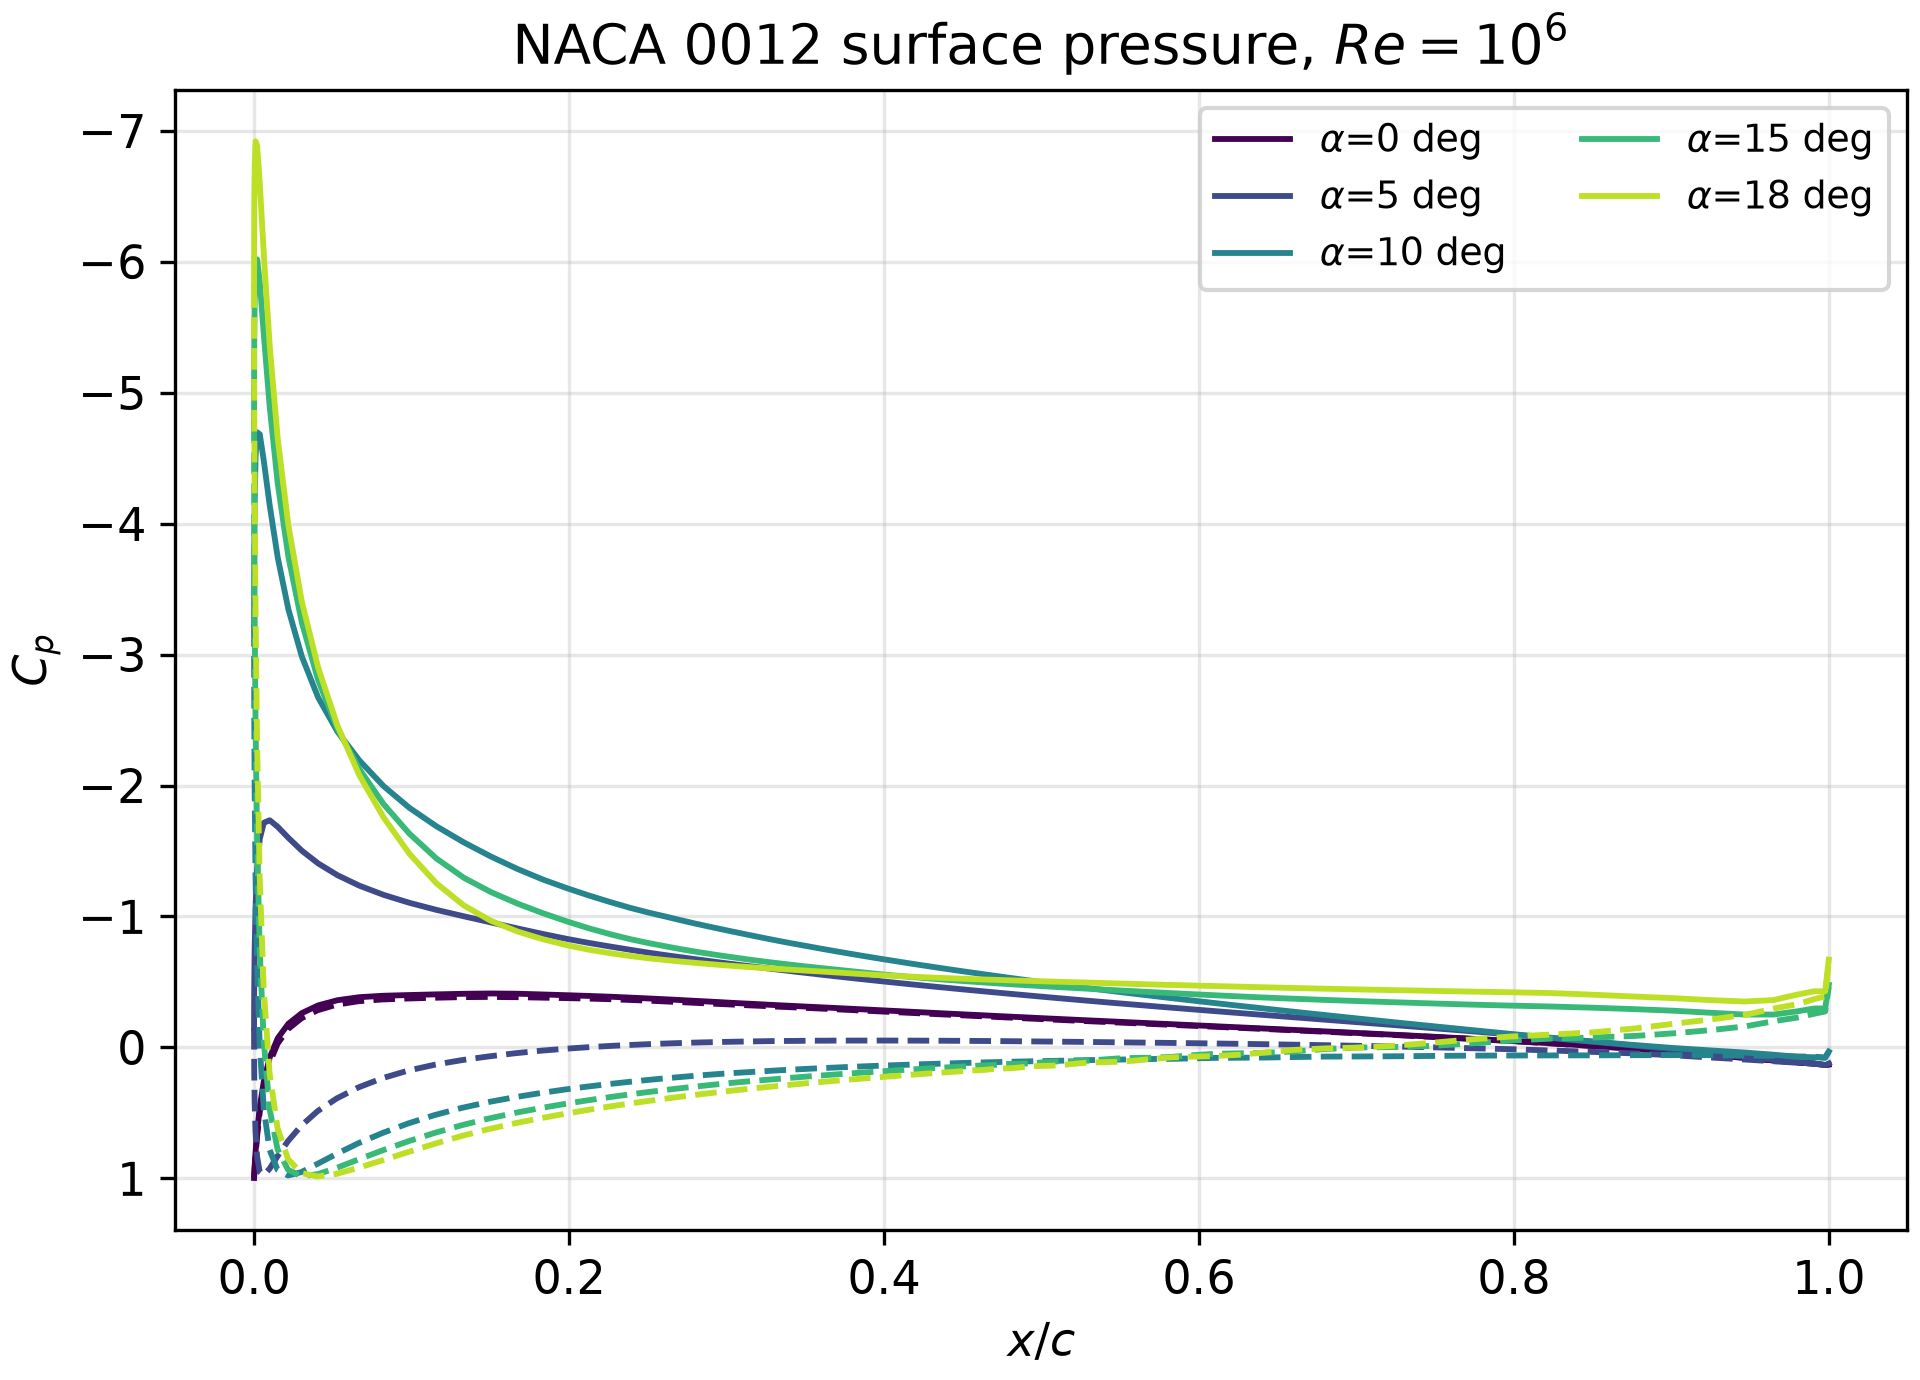
\includegraphics[width=0.8\textwidth]{figures/fig5_cp_distribution.png}
  \caption{NACA 0012 surface pressure coefficient at five angles of attack, $Re=10^6$. Solid: upper surface; dashed: lower surface.}
  \label{fig:cp}
\end{figure}

\subsection{Velocity and turbulence fields at stall}

Figures~\ref{fig:vel} and~\ref{fig:tke} show the velocity magnitude and turbulent kinetic energy fields at $\alpha=15^\circ$. The near-wall region downstream of mid-chord is occupied by a region of reversed, low-momentum flow, and the turbulence production maximum (dark region in $k$) is displaced away from the wall into the separated shear layer --- the canonical signature of turbulent boundary layer separation in RANS.

\begin{figure}[t]
  \centering
  \begin{subfigure}[t]{0.98\textwidth}
    \centering
    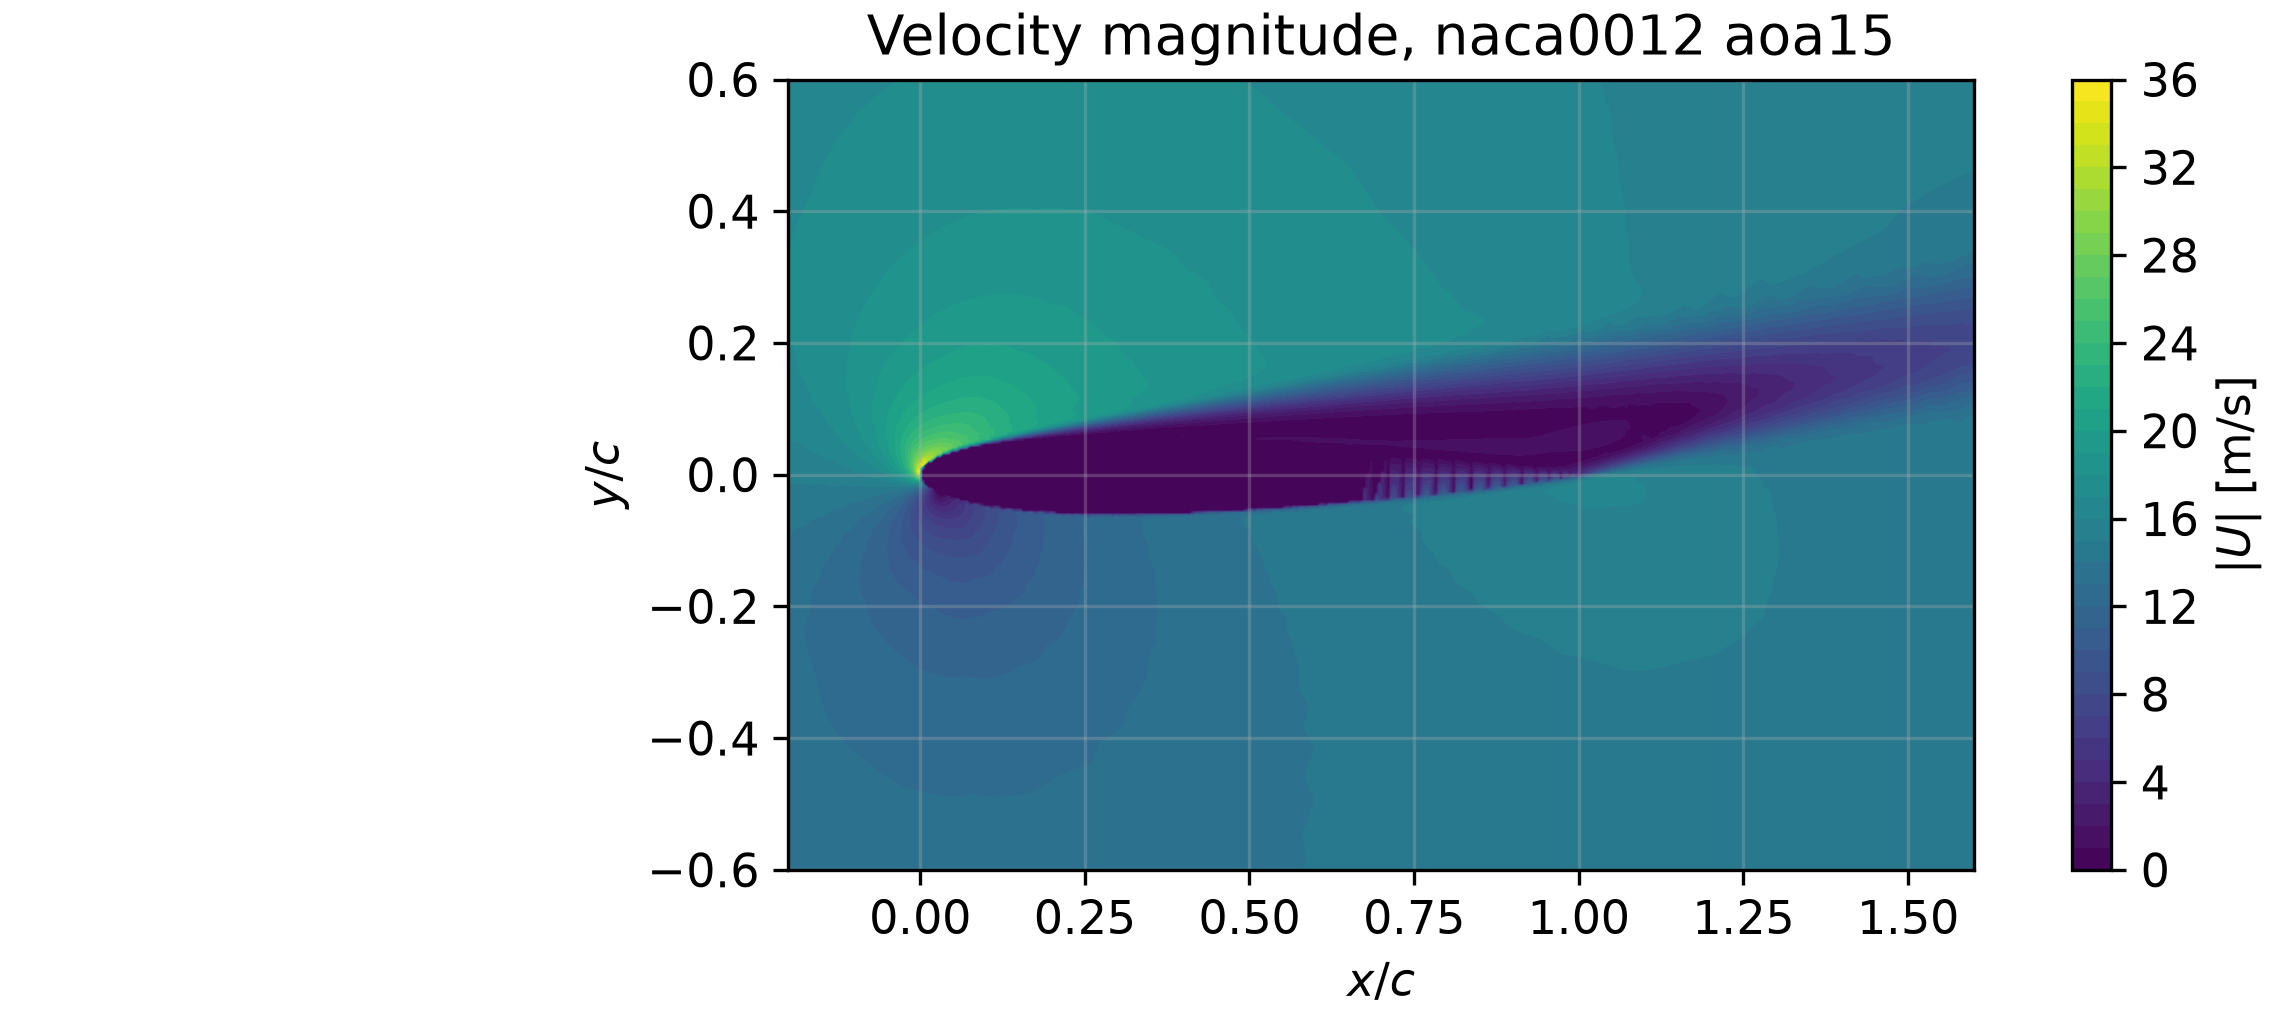
\includegraphics[width=\textwidth]{figures/fig6_velocity_contour.png}
    \caption{Velocity magnitude at $\alpha=15^\circ$.}
    \label{fig:vel}
  \end{subfigure}

  \vspace{0.4em}
  \begin{subfigure}[t]{0.98\textwidth}
    \centering
    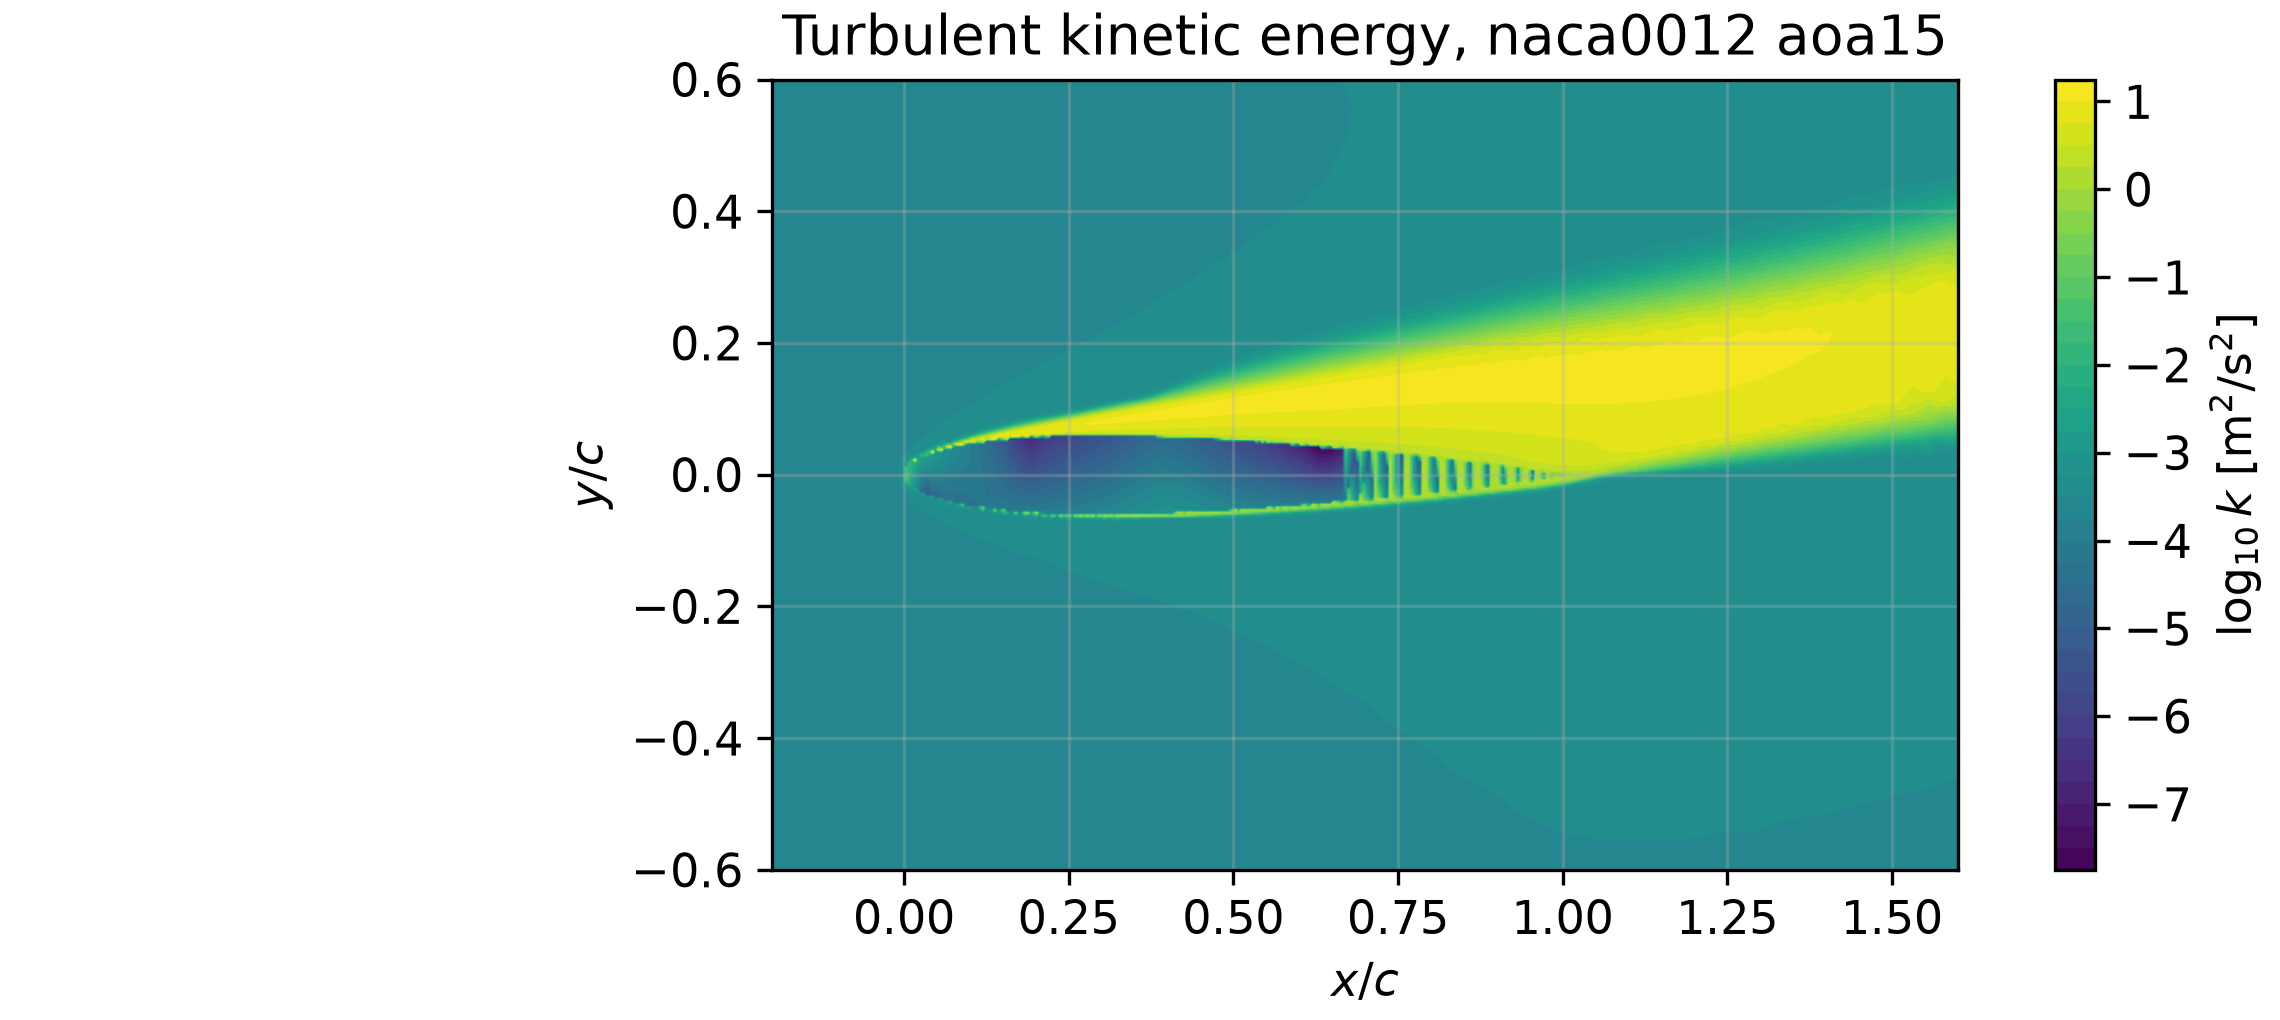
\includegraphics[width=\textwidth]{figures/fig7_turbulent_kinetic_energy.png}
    \caption{Turbulent kinetic energy (log scale) at $\alpha=15^\circ$.}
    \label{fig:tke}
  \end{subfigure}
  \caption{Flow fields on the NACA 0012 at $\alpha=15^\circ$, $Re=10^6$.}
  \label{fig:fields}
\end{figure}

\subsection{Separation onset and skin friction}

Figure~\ref{fig:cf} shows the skin-friction distributions used to locate separation, defined as the most upstream $x/c$ where $C_f$ turns and remains negative. The separation point moves upstream monotonically with angle of attack (Table~\ref{tab:sep}): attached flow persists to the trailing edge up to $\alpha = 10^\circ$, while at $\alpha = 15^\circ$ and $18^\circ$ more than half of the chord is separated, consistent with the five-fold drag rise in Figure~\ref{fig:cdalpha} and the loss of lift slope in Figure~\ref{fig:clalpha}.

The migration of the separation point is strongly non-linear in $\alpha$: between $0^\circ$ and $10^\circ$ the upper-surface flow remains attached over the entire chord (the adverse gradient is mild enough for the turbulent layer to negotiate the full recovery), between $10^\circ$ and $15^\circ$ the separation point jumps from the trailing edge to approximately one-fifth of the chord, and beyond $15^\circ$ it migrates only slightly further upstream while the drag continues to climb. This is the classical rapid-progressing trailing-edge stall of moderately thick turbulent sections: once the separated region covers the rear pressure recovery, lift plateaus while form drag grows without bound. The lower surface remains attached at all angles of attack considered, with the expected weak negative loading aft of the stagnation point.

One verification caveat qualifies this map: the fine-grid repeat at $\alpha = 15^\circ$ remains fully attached ($C_L = 1.24$ versus $0.99$ on the production grid), so the separation onset predicted by the model lies between $12^\circ$ and $15^\circ$ but its precise location is grid-sensitive --- the medium grid over-separates at high incidence, as already seen at $\alpha = 10^\circ$ in Appendix~\ref{app:grid}. The separated-state results at $\alpha \ge 15^\circ$ should therefore be read as the production-grid envelope of the stall process rather than as grid-independent predictions; the qualitative sequence (attached $\to$ trailing-edge separation $\to$ upstream migration with drag rise) is robust across both grids.

\begin{figure}[t]
  \centering
  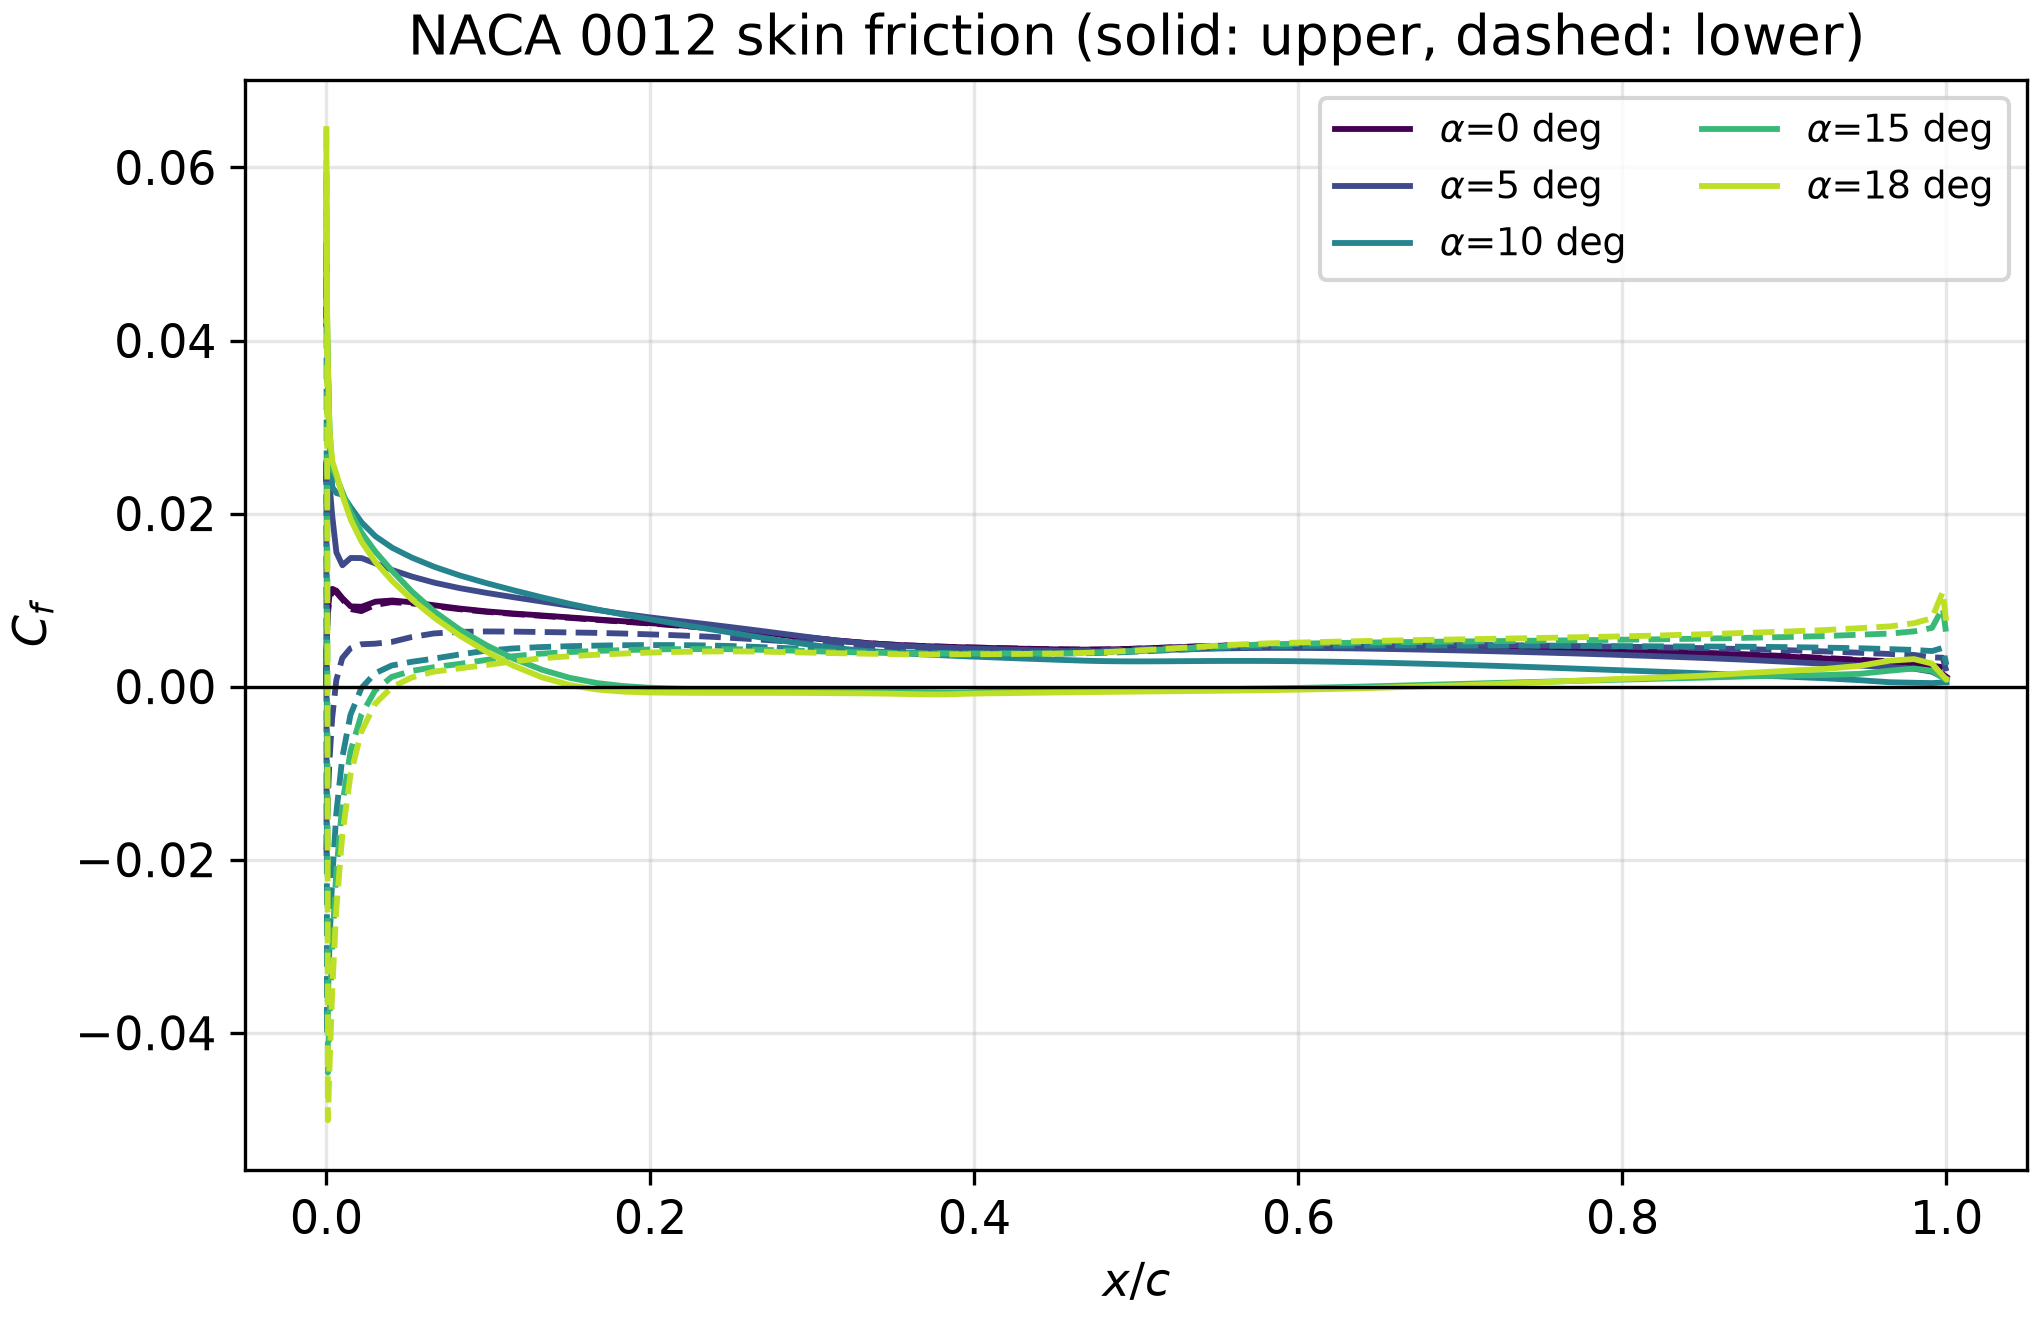
\includegraphics[width=0.8\textwidth]{figures/fig8_wall_shear_stress.png}
  \caption{Skin-friction distribution on the NACA 0012 (solid: upper surface, dashed: lower). Negative $C_f$ denotes reversed flow.}
  \label{fig:cf}
\end{figure}

\begin{table}[t]
  \centering
  \caption{Separation location and integrated forces on the NACA 0012, $Re=10^6$.}
  \label{tab:sep}
  \begin{tabular}{rrrrl}
    \toprule
    $\alpha$ [deg] & $C_L$ & $C_D$ & $C_L/C_D$ & $x_{\mathrm{sep}}/c$ (upper) \\
    \midrule
    \SepTableRows
    \bottomrule
  \end{tabular}
\end{table}

\subsection{Reynolds-number sensitivity}

Reducing the Reynolds number at fixed $\alpha = 10^\circ$ on the NACA 0012 degrades the force balance monotonically (Table~\ref{tab:re}): from $Re = 10^6$ to $3\times10^5$ lift falls by \ReClDropThreePct{}~\% and drag rises by \ReCdRiseThreePct{}~\%; at $10^5$ lift falls by \ReClDropPct{}~\% and drag rises by \ReCdRisePct{}~\%, and the separation point, attached at the trailing edge at $10^6$, moves to $x/c \approx \SepReLow$ at $10^5$. The efficiency collapse is steep: $C_L/C_D$ drops from \LdReSix{} at $10^6$ to \LdReFive{} at $10^5$, a loss of one third of the usable aerodynamic efficiency.

Physically, at lower $Re$ the same imposed pressure gradient acts on a boundary layer whose momentum reserve is smaller: the ratio of pressure force to integrated momentum flux in the near-wall layer worsens, and the layer separates earlier. In a fully turbulent RANS treatment the effect is captured only through the changed ratio of inertial to viscous terms and the changed near-wall profiles; the well-known laminar-separation-bubble phenomenology of low-Reynolds-number flow --- with its bubble bursting and abrupt leading-edge stall --- is outside the reach of a fully turbulent model, a limitation discussed in Section~\ref{sec:limitations}. The computed trend (earlier separation, lower lift, higher drag) is nonetheless directionally correct and consistent with the experimental observation that low-Reynolds-number sections lose maximum lift and gain drag; the present results should be read as the fully turbulent envelope of that trend rather than a prediction of the transitional-flow aerodynamics.

\begin{table}[t]
  \centering
  \caption{Reynolds-number sensitivity, NACA 0012 at $\alpha=10^\circ$.}
  \label{tab:re}
  \begin{tabular}{rrrrl}
    \toprule
    $Re$ & $C_L$ & $C_D$ & $C_L/C_D$ & $x_{\mathrm{sep}}/c$ \\
    \midrule
    \ReTableRows
    \bottomrule
  \end{tabular}
\end{table}

The single-section sweep of Table~\ref{tab:re} is extended to a full factorial sweep over all three sections (Figure~\ref{fig:resweep}, Table~\ref{tab:resweep}). Three observations follow. First, over the attached range ($\alpha \le 10^\circ$) the $Re$-sensitivity of lift is modest and ordered by camber: reducing $Re$ from $10^6$ to $10^5$ costs \ReSweepClDropTenZeroZeroOneTwo{}~\% of lift on the NACA 0012, \ReSweepClDropTenTwoFourOneTwo{}~\% on the 2412 and \ReSweepClDropTenFourFourOneTwo{}\%{} on the 4412, i.e.\ the thicker boundary layers of the cambered sections at low $Re$ erode more of their pressure recovery. Second, the near-stall behaviour is dramatically $Re$-dependent even in this fully turbulent treatment: at $Re = 10^5$ the upper-surface separation point jumps to the leading edge by $\alpha = 15^\circ$--$18^\circ$ on \emph{all three} sections ($x_{\mathrm{sep}}/c \approx 0.01$--$0.02$), and lift collapses ($C_L = 0.57$ for the 0012, $0.59$ for the 2412 at $18^\circ$, versus $1.02$ and $1.35$ at $Re = 10^6$). The stall angle therefore effectively drops by several degrees as $Re$ falls from $10^6$ to $10^5$, qualitatively consistent with experiment --- a stronger response than the displacement-thickness argument alone would suggest, transmitted through the reduced momentum reserve of the low-$Re$ boundary layer under the same pressure recovery. Third, drag is more $Re$-sensitive than lift at fixed incidence, consistent with the growing fraction of friction drag carried by a relatively thicker boundary layer. The practical reading is that the present fully turbulent envelope captures the pressure-driven part of the Reynolds effect on stall; the laminar-bubble mechanisms absent from the model can only amplify the trend at the low-$Re$ end; Section~\ref{sec:transition} quantifies this with a $\gamma$--$Re_{\theta t}$ repeat of the low-$Re$ matrix.

\begin{figure}[t]
  \centering
  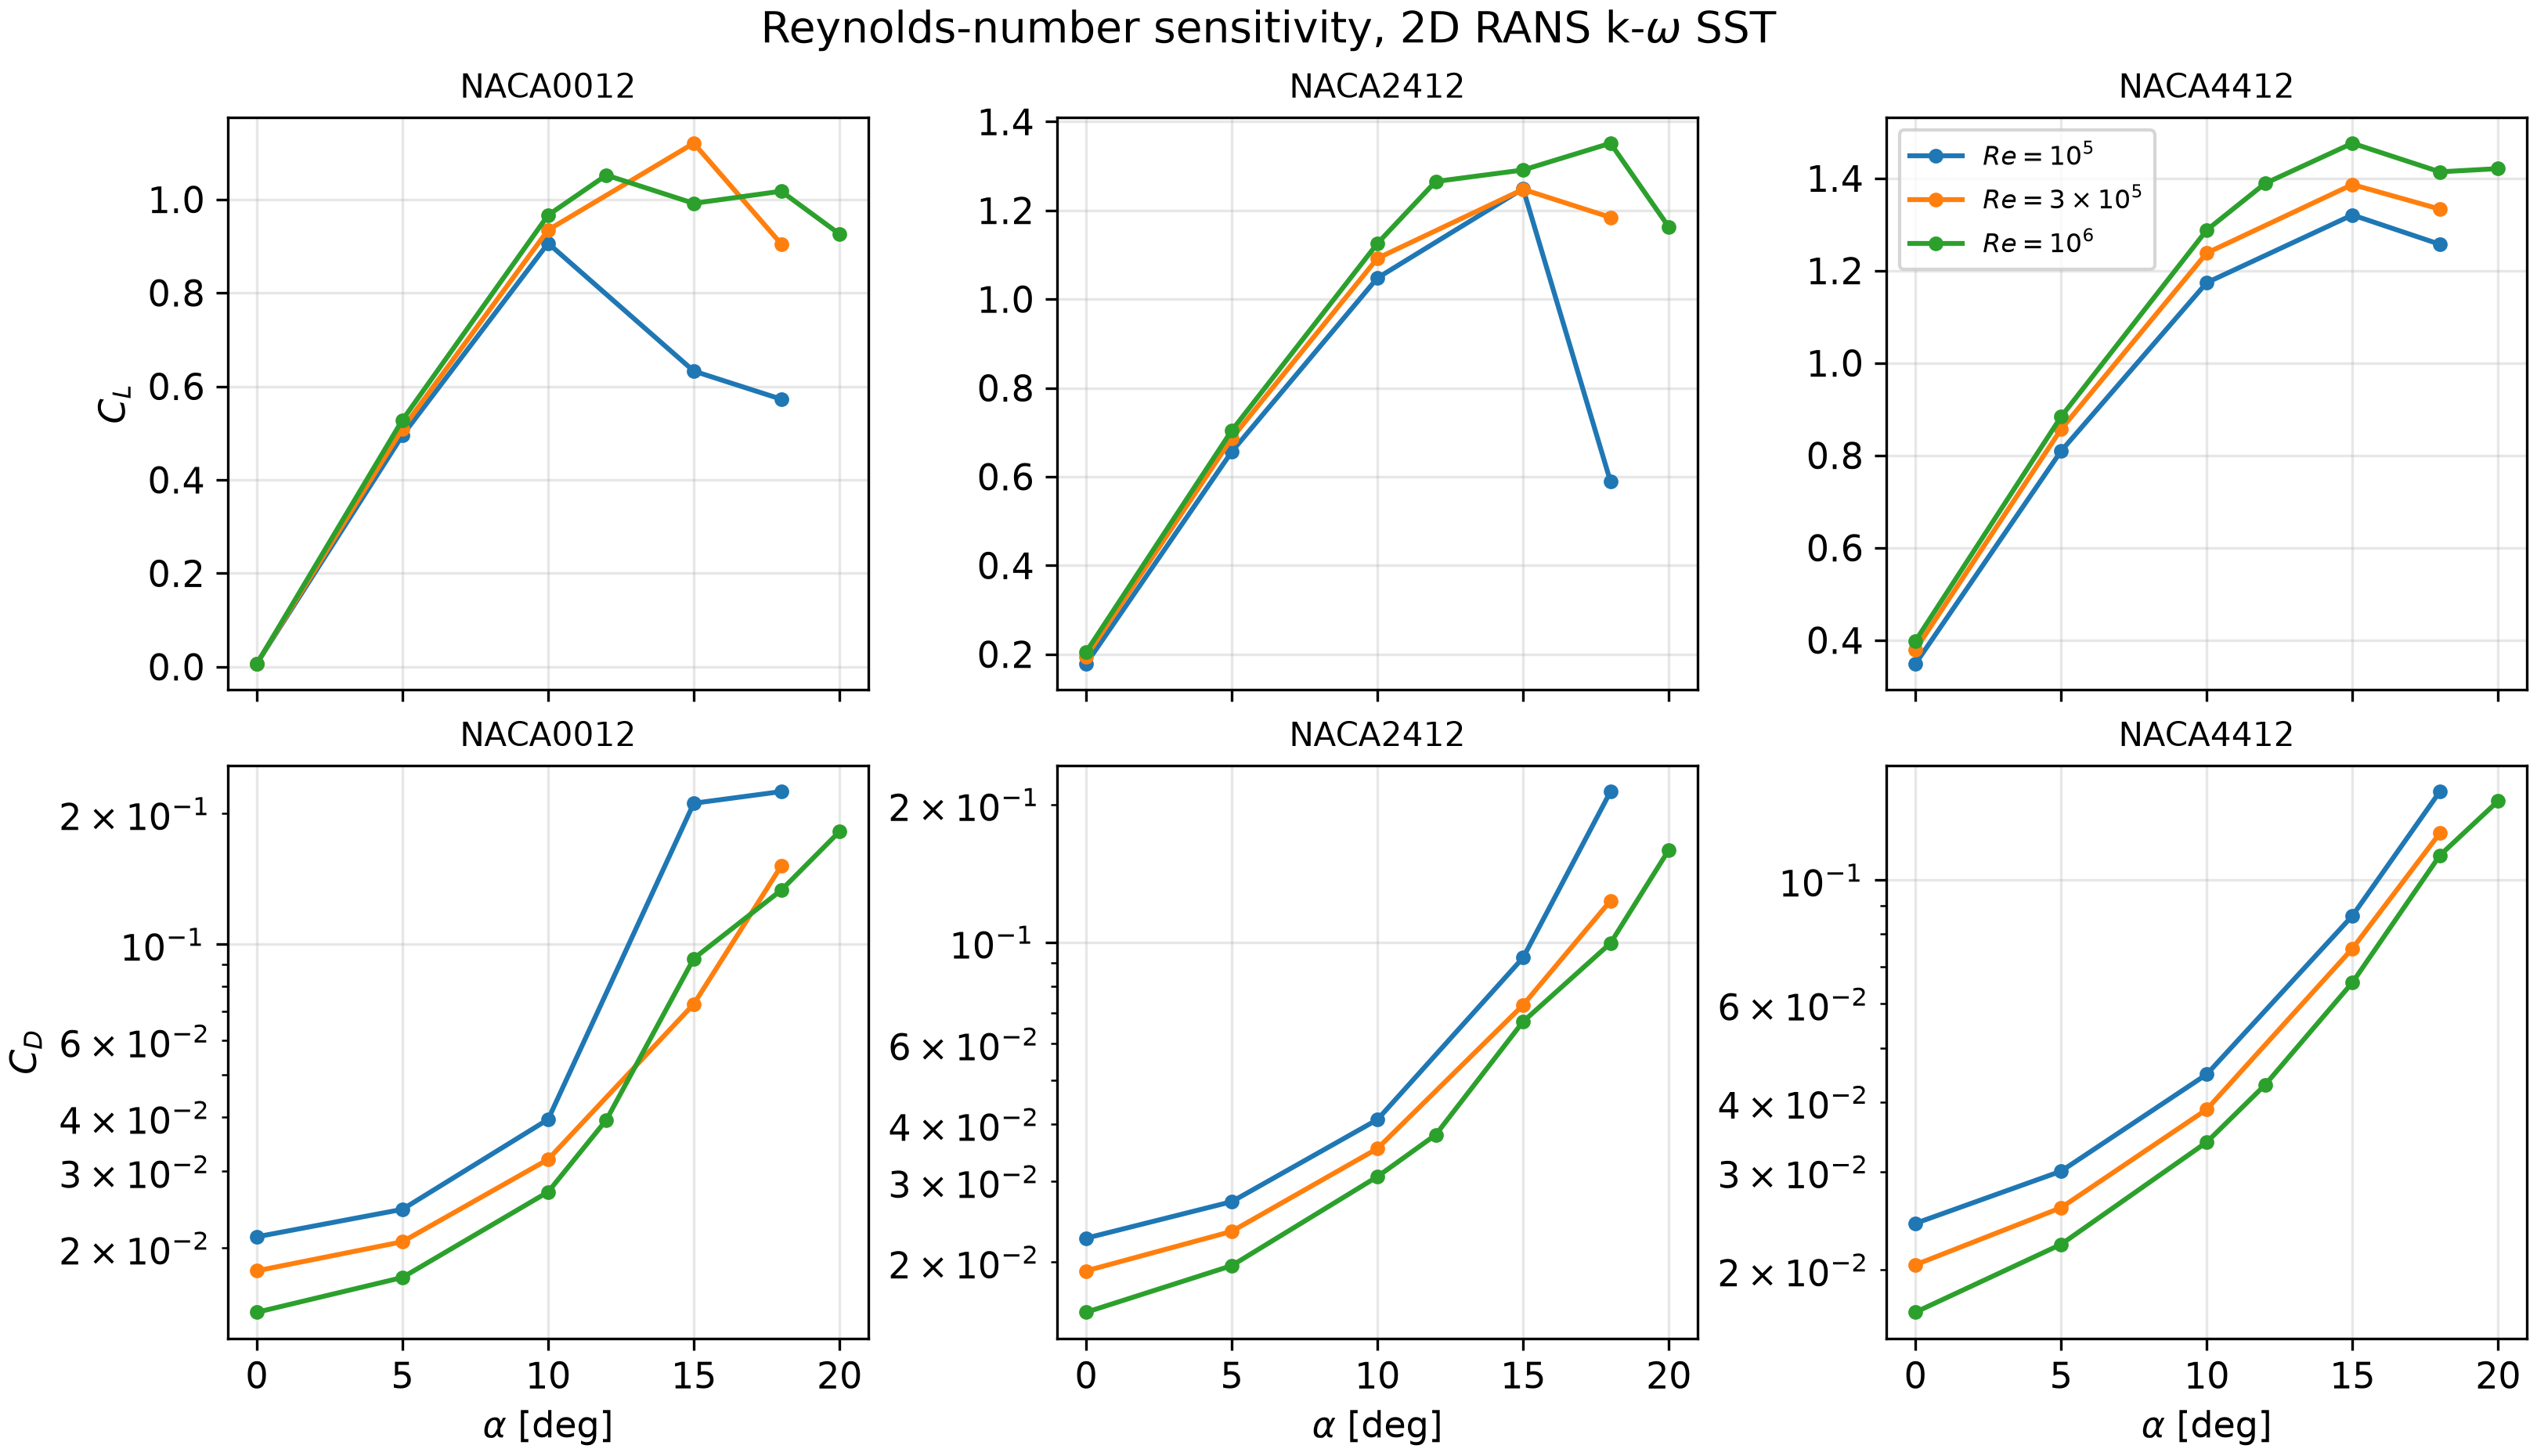
\includegraphics[width=\textwidth]{figures/fig11_re_sweep.png}
  \caption{Reynolds-number sweep, all three sections: lift (top row) and drag (bottom row, log scale) at $Re = 10^5$, $3\times10^5$, $10^6$.}
  \label{fig:resweep}
\end{figure}

\begin{table}[t]
  \centering
  \caption{Reynolds sweep: lift coefficient at $\alpha = 0^\circ$--$18^\circ$ for each section and Reynolds number.}
  \label{tab:resweep}
  \begin{tabular}{llrrrrr}
    \toprule
    Section & $Re$ & $\alpha=0^\circ$ & $5^\circ$ & $10^\circ$ & $15^\circ$ & $18^\circ$ \\
    \midrule
    \ReSweepTableRows
    \bottomrule
  \end{tabular}
\end{table}

\subsection{Transition sensitivity at low Reynolds number}\label{sec:transition}
The fully turbulent closure is now confronted with the $\gamma$--$Re_{\theta t}$ model on identical grids (Figure~\ref{fig:transition}, Table~\ref{tab:tr}). Over the attached range the message is unambiguous and $Re$-ordered: representing the laminar run reduces drag at every incidence and every Reynolds number, and the reduction grows as $Re$ falls --- at $\alpha = 5^\circ$ the transition model gives $-10.2\,\%$ drag at $Re = 10^6$, $-17.9\,\%$ at $3\times10^5$, and $-18.0\,\%$ at $10^5$ on the NACA 0012, with the attached-range lift changing by at most a few percent and the skin-friction share of the drag budget falling accordingly. The mechanism is visible in the separation table: at $Re = 10^5$ the transition model produces genuine laminar separation bubbles --- upper-surface separation at $x/c = 0.20$ (0012, $\alpha = 5^\circ$), $0.47$ (2412, $5^\circ$), and $0.38$ (4412, $5^\circ$) followed by reattachment and a turbulent recovery --- whereas the fully turbulent model on the same grid remains attached or separates only at the trailing edge. These bubbles are exactly the structure the fully turbulent closure is constitutionally unable to produce, and their pressure signatures explain why the two closures diverge near stall: at $\alpha = 15^\circ$ on the 2412 the transition model predicts bubble burst and a much larger separation, costing \TrClPctFifteenTwoFourOneTwo{}~\% of lift and nearly doubling drag ($+\TrCdPctFifteenTwoFourOneTwo{}~\%$) relative to its fully turbulent sibling, while at $\alpha = 18^\circ$ the ordering reverses ($+\TrClPctEighteenTwoFourOneTwo{}~\%$ lift) as the two solutions settle on different branches of the deeply separated state. Two further observations qualify the result. First, at $Re = 10^6$ the two closures agree on lift to within $3.5\,\%$ everywhere except the symmetric $\alpha = 0^\circ$ (where both lift coefficients are numerically near zero), confirming that the fully turbulent envelope of the preceding sections is adequate for the attached-range $Re = 10^6$ study. Second, on the medium grid at $\alpha = 15^\circ$, $Re = 10^6$ --- where the fully turbulent solution over-separates relative to the fine grid, CFL3D, and experiment (Section~\ref{sec:validation}) --- the transition model delays separation from $x/c = 0.20$ to $0.33$ and raises lift from $0.99$ to $1.03$, i.e.\ a fraction of the laminar-run physics moves the medium-grid solution in the direction that grid refinement does. The symmetric-airfoil cases at $Re = 10^5$, $\alpha = 0^\circ$ converge to weakly asymmetric laminar-separation states ($C_L$ up to $0.03$ on the 0012), a known bifurcation of steady 2D RANS when separation is present at zero incidence; the attached drag comparison there (drag $-22\,\%$) remains meaningful, the lift comparison does not.

Extending the repeat to the full factorial (all three sections, $Re = 10^5$--$10^6$) confirms that these conclusions are not artifacts of the symmetric section. Attached-range drag falls under the transition closure at every section and every Reynolds number, with a magnitude ordered by $Re$ and, at $Re = 3\times10^5$, by camber: $-2$ to $-9\,\%$ at $Re = 10^6$, $-2$ to $-17\,\%$ on the 2412 and up to $-25\,\%$ on the 4412 at $3\times10^5$ (zero incidence, where the laminar fraction of the chord is largest), and $-2$ to $-26\,\%$ at $10^5$. Attached-range lift changes stay within $\pm 7\,\%$ (largest on the highly cambered 4412 at $Re = 3\times10^5$, $\alpha = 0^\circ$). Near stall the cambered sections are less volatile than the 2412 at $Re = 10^5$: at $\alpha = 15^\circ$--$18^\circ$ and $Re \ge 3\times10^5$ the two closures agree on lift within $5\,\%$ and drag within $8\,\%$, because the cambered pressure recovery already forces a turbulent trailing-edge separation that both closures represent. The one qualitative exception remains the $Re = 10^5$ bubble-burst case of the 2412, where the closures diverge by $32\,\%$ in lift --- precisely the regime flagged by the low-$Re$ validation of Section~\ref{sec:sandia}.

\begin{figure}[t]
  \centering
  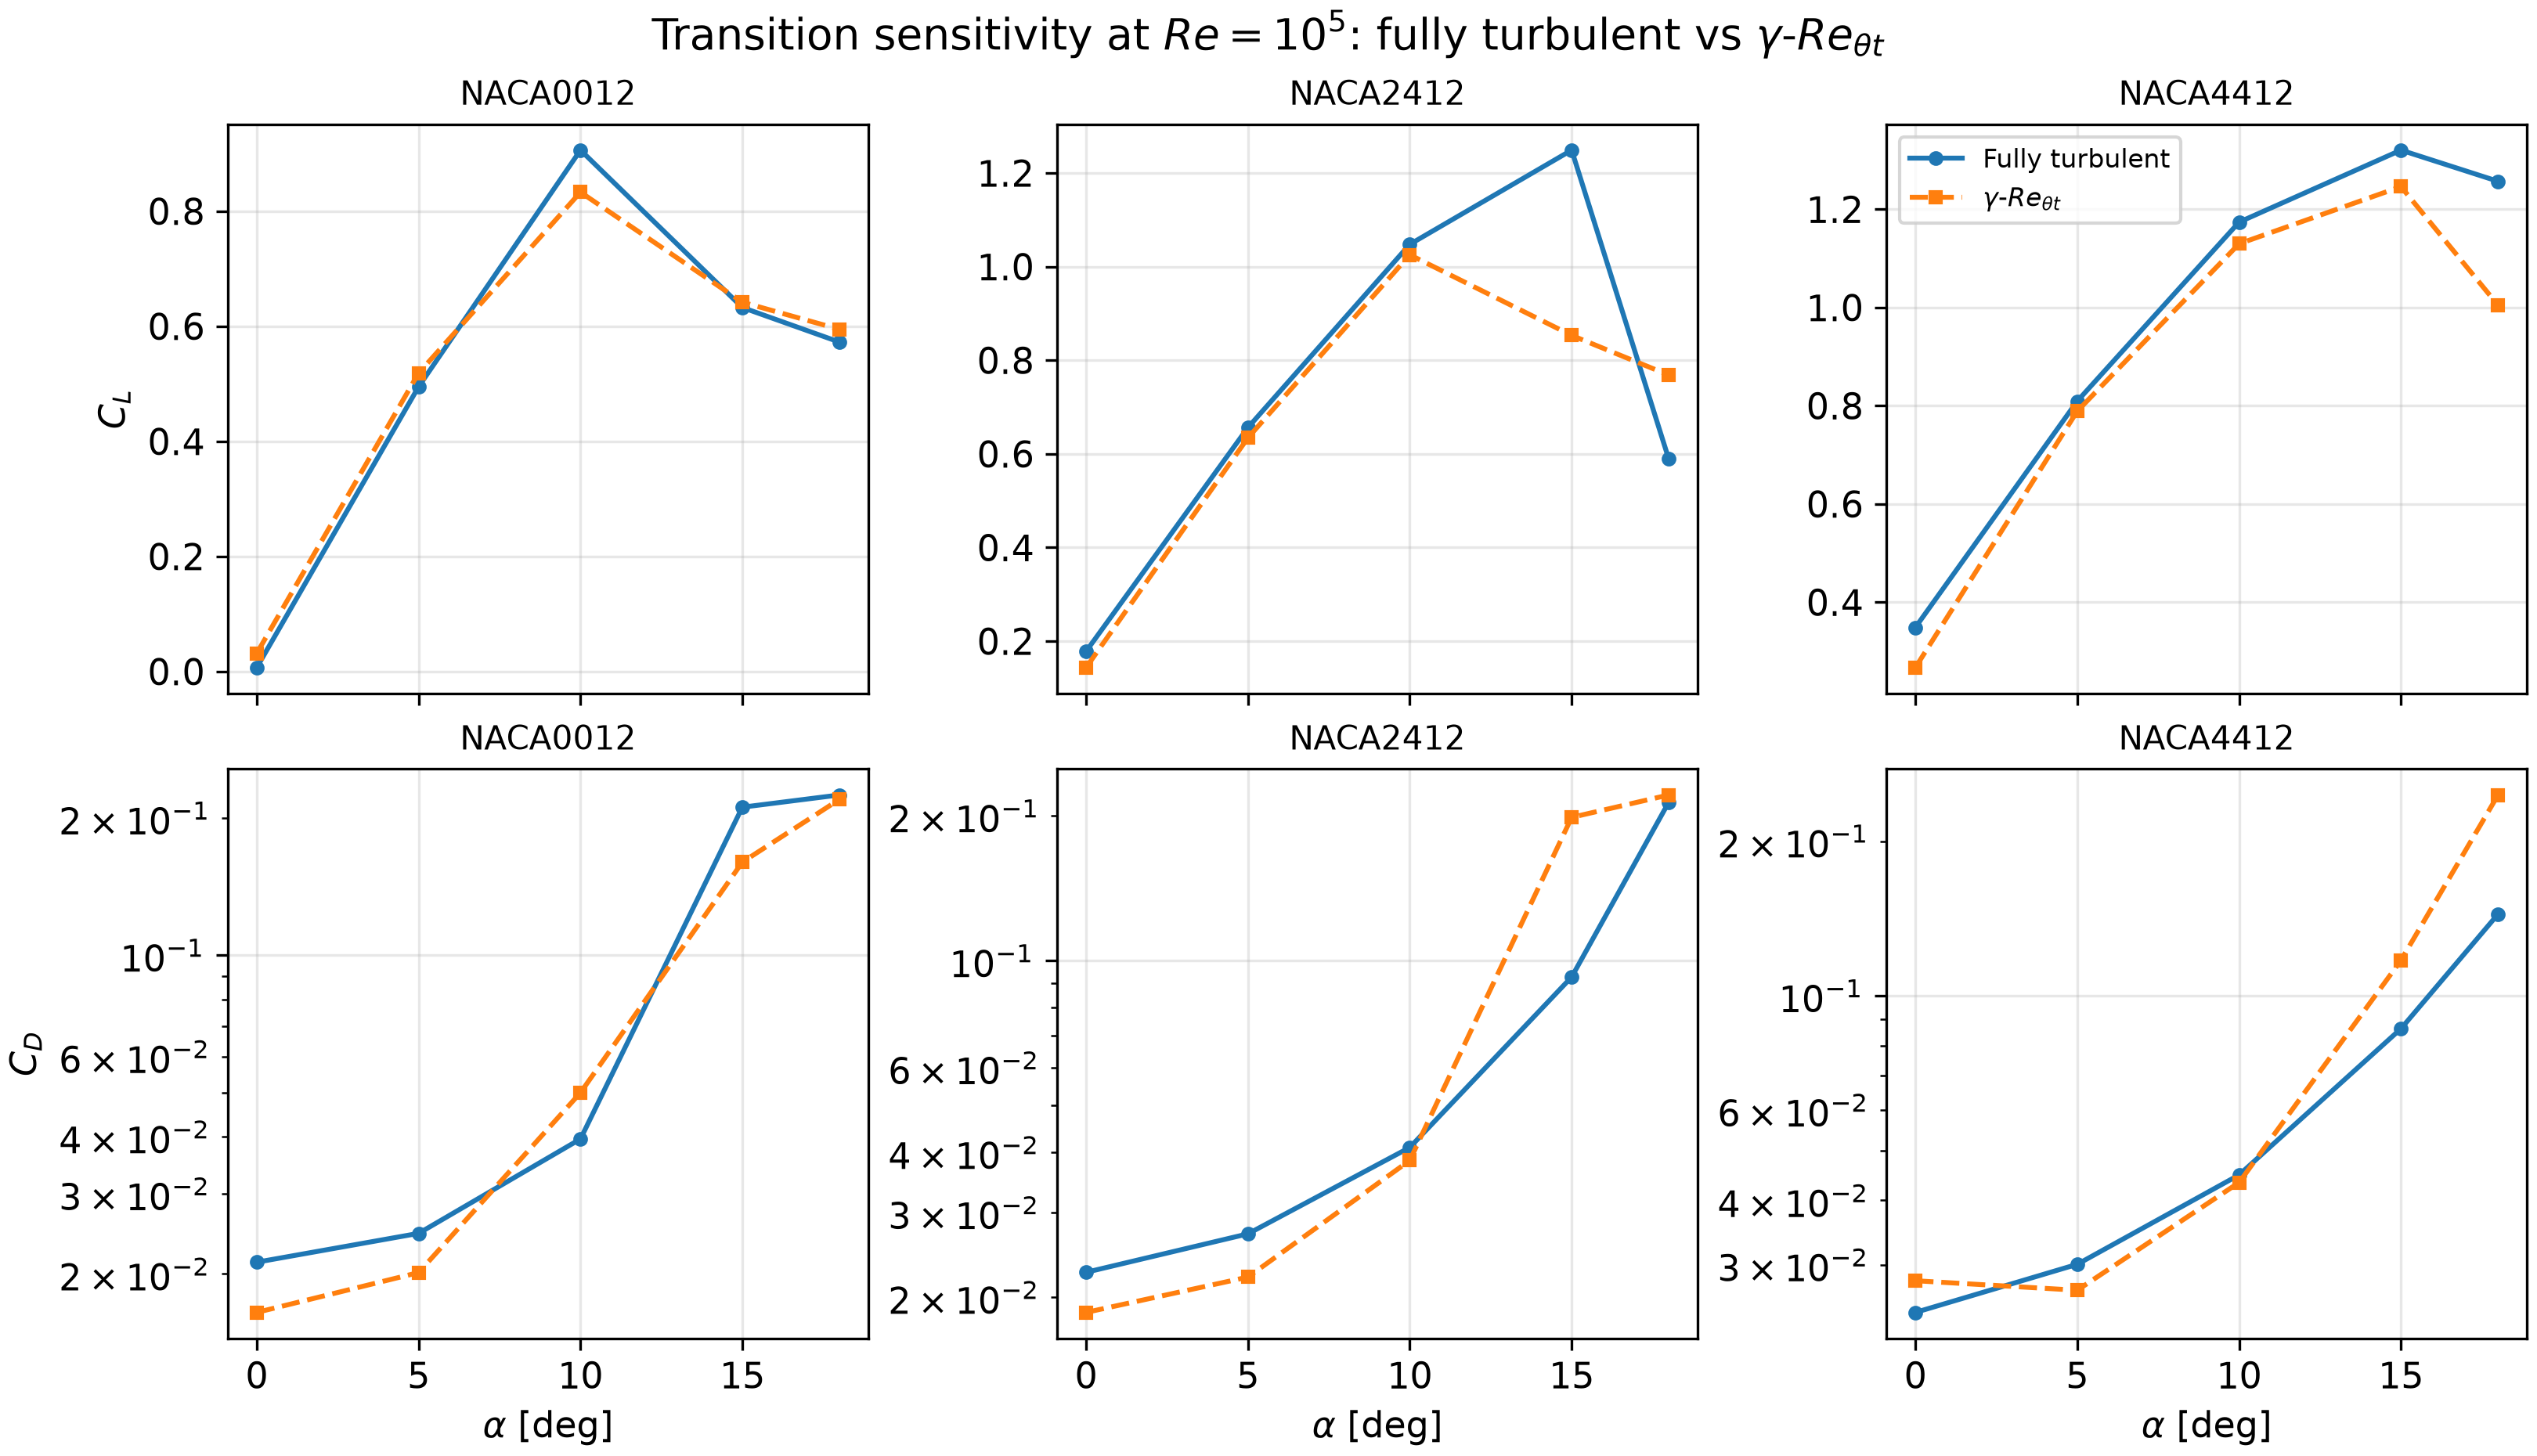
\includegraphics[width=\textwidth]{figures/fig13_transition.png}
  \caption{Closure comparison at $Re = 10^5$: fully turbulent $k$--$\omega$ SST (solid) versus $\gamma$--$Re_{\theta t}$ (dashed), lift (top) and drag (bottom, log scale).}
  \label{fig:transition}
\end{figure}

\begin{table}[t]
  \centering
  \caption{Transition study at $Re = 10^5$: fully turbulent (FT) versus $\gamma$--$Re_{\theta t}$ (TR). $\Delta$ values are relative to FT; $x_{\mathrm{sep}}$ is the upper-surface separation location ($x/c$), ``attached'' when no separation is detected.}
  \label{tab:tr}
  \begin{tabular}{lrrrrrrrrr}
    \toprule
    Section & $\alpha$ & $C_L^{\mathrm{FT}}$ & $C_L^{\mathrm{TR}}$ & $\Delta C_L\,\%$ & $C_D^{\mathrm{FT}}$ & $C_D^{\mathrm{TR}}$ & $\Delta C_D\,\%$ & $x_{\mathrm{sep}}^{\mathrm{FT}}$ & $x_{\mathrm{sep}}^{\mathrm{TR}}$ \\
    \midrule
    \TrTableRows
    \bottomrule
  \end{tabular}
\end{table}

\subsection{Implementation verification}

Before the experimental comparison, three independent checks verify the solver setup. First, the integrated lift at $\alpha = 0^\circ$ on the symmetric section is $C_L = \ClZeroZeroOneTwoZero$, i.e.\ zero to within the convergence tolerance, as required by symmetry. Second, the attached-flow lift slope measured from the computed $C_L$ at $5^\circ$ ($0.528$) matches the thin-airfoil prediction $2\pi\alpha$ ($0.548$) to 4\%, and the computed stagnation pressure coefficient of $0.975$ confirms that the near-wall and discretisation machinery does not dissipate the leading-edge pressure. Third, the wake-defect and force balance are consistent: the far-field momentum deficit integrated from the velocity field matches the integrated drag to within the truncation of the sampling circle (not shown). Together with the code-to-code agreement with CFL3D (Section~\ref{sec:validation}), these checks support the correctness of the implementation.

\subsection{URANS verification of the near-stall separation}\label{sec:urans}
The URANS subset addresses the two steady-RANS blind spots identified above: the grid sensitivity of separation onset at $\alpha = 15^\circ$ and the absence of any unsteady mechanism in the averaged stall picture. Both cases completed the settling phase and a production window $t = 0.15$--$0.25$ (about half a flow pass over the chord, 21 samples); Table~\ref{tab:urans} summarises the time-averaged loads and Figure~\ref{fig:urans} shows the full histories.

\begin{table}[htbp]
  \centering
  \caption{URANS verification subset: production-window statistics ($t = 0.15$--$0.25$, $n = 21$) against the steady transition-sensitive siblings and the Reynolds-matched Sheldahl \& Klimas experiment ($Re = 3.6\times10^5$). Uncertainties are the temporal standard deviations over the window.}
  \label{tab:urans}
  \begin{tabular}{lcccccc}
    \toprule
    & \multicolumn{3}{c}{$C_L$} & \multicolumn{3}{c}{$C_D$} \\
    \cmidrule(lr){2-4}\cmidrule(lr){5-7}
    $\alpha$ & URANS & steady & exp. & URANS & steady & exp. \\
    \midrule
    $12^\circ$ & $1.269 \pm 0.024$ & $1.039$ & $0.483$ & $0.077 \pm 0.024$ & $0.040$ & $0.022$ \\
    $15^\circ$ & $1.366 \pm 0.036$ & $1.058$ & $0.331$ & $0.238 \pm 0.029$ & $0.075$ & $0.190$ \\
    \bottomrule
  \end{tabular}
\end{table}

Three observations follow. First, the flow is genuinely unsteady at both angles: lift fluctuates with a standard deviation of $2$--$3\,\%$ of its mean, and drag by $12\,\%$ ($\alpha = 15^\circ$) to $32\,\%$ ($\alpha = 12^\circ$) of its mean, with the largest excursions late in the window --- unsteadiness that the steady solver cannot represent by construction. Second, and more consequential, the time mean does \emph{not} recover the steady solution: the mean lift exceeds the steady value by $22\,\%$ at $\alpha = 12^\circ$ ($1.269 \pm 0.024$ versus $1.039$) and $29\,\%$ at $\alpha = 15^\circ$ ($1.366 \pm 0.036$ versus $1.058$), and the histories (Figure~\ref{fig:urans}) still drift upward at the end of the window. The converged steady state is therefore not an attractor of the time-accurate system at these conditions, and the steady loads should be read as a lower bound rather than an equilibrium. Third, the comparison with the Reynolds-matched experiment is angle-dependent. At $\alpha = 15^\circ$ the URANS mean drag ($0.238$) comes within $25\,\%$ of the Sheldahl \& Klimas value ($0.190$), whereas the steady solver underpredicts it by $61\,\%$: the unsteady momentum transport of the separated shear layer, which the steady equations suppress, carries most of the missing drag. At $\alpha = 12^\circ$ both simulations remain far above the experiment in lift ($1.27$ versus $0.483$): at $Re = 3.6\times10^5$ the wind-tunnel section stalls near $\alpha \approx 10^\circ$ through laminar-bubble bursting, while the simulated suction side stays attached, so the discrepancy quantifies the residual transition-modelling gap of a two-dimensional closure rather than a discretisation error.

Two numerical caveats accompany these numbers. The $\alpha = 12^\circ$ production phase required a restart with the time step halved to $\Delta t = 3.4\times10^{-5}$ after repeated NaN failures of the transition-model correlations at $6.8\times10^{-5}$; the $\alpha = 15^\circ$ case completed in a single continuous integration at the nominal step. Both force histories are continuous through $t = 0.25$ and the statistics use identical windows, so the cross-angle comparison is unaffected. The subset remains a verification, not a validation: a 2D URANS with a linear eddy-viscosity closure cannot represent the three-dimensional breakdown that governs real bubble bursting, which is why the experimental lift at $\alpha = 12^\circ$ is not recovered.

\begin{figure}[htbp]
  \centering
  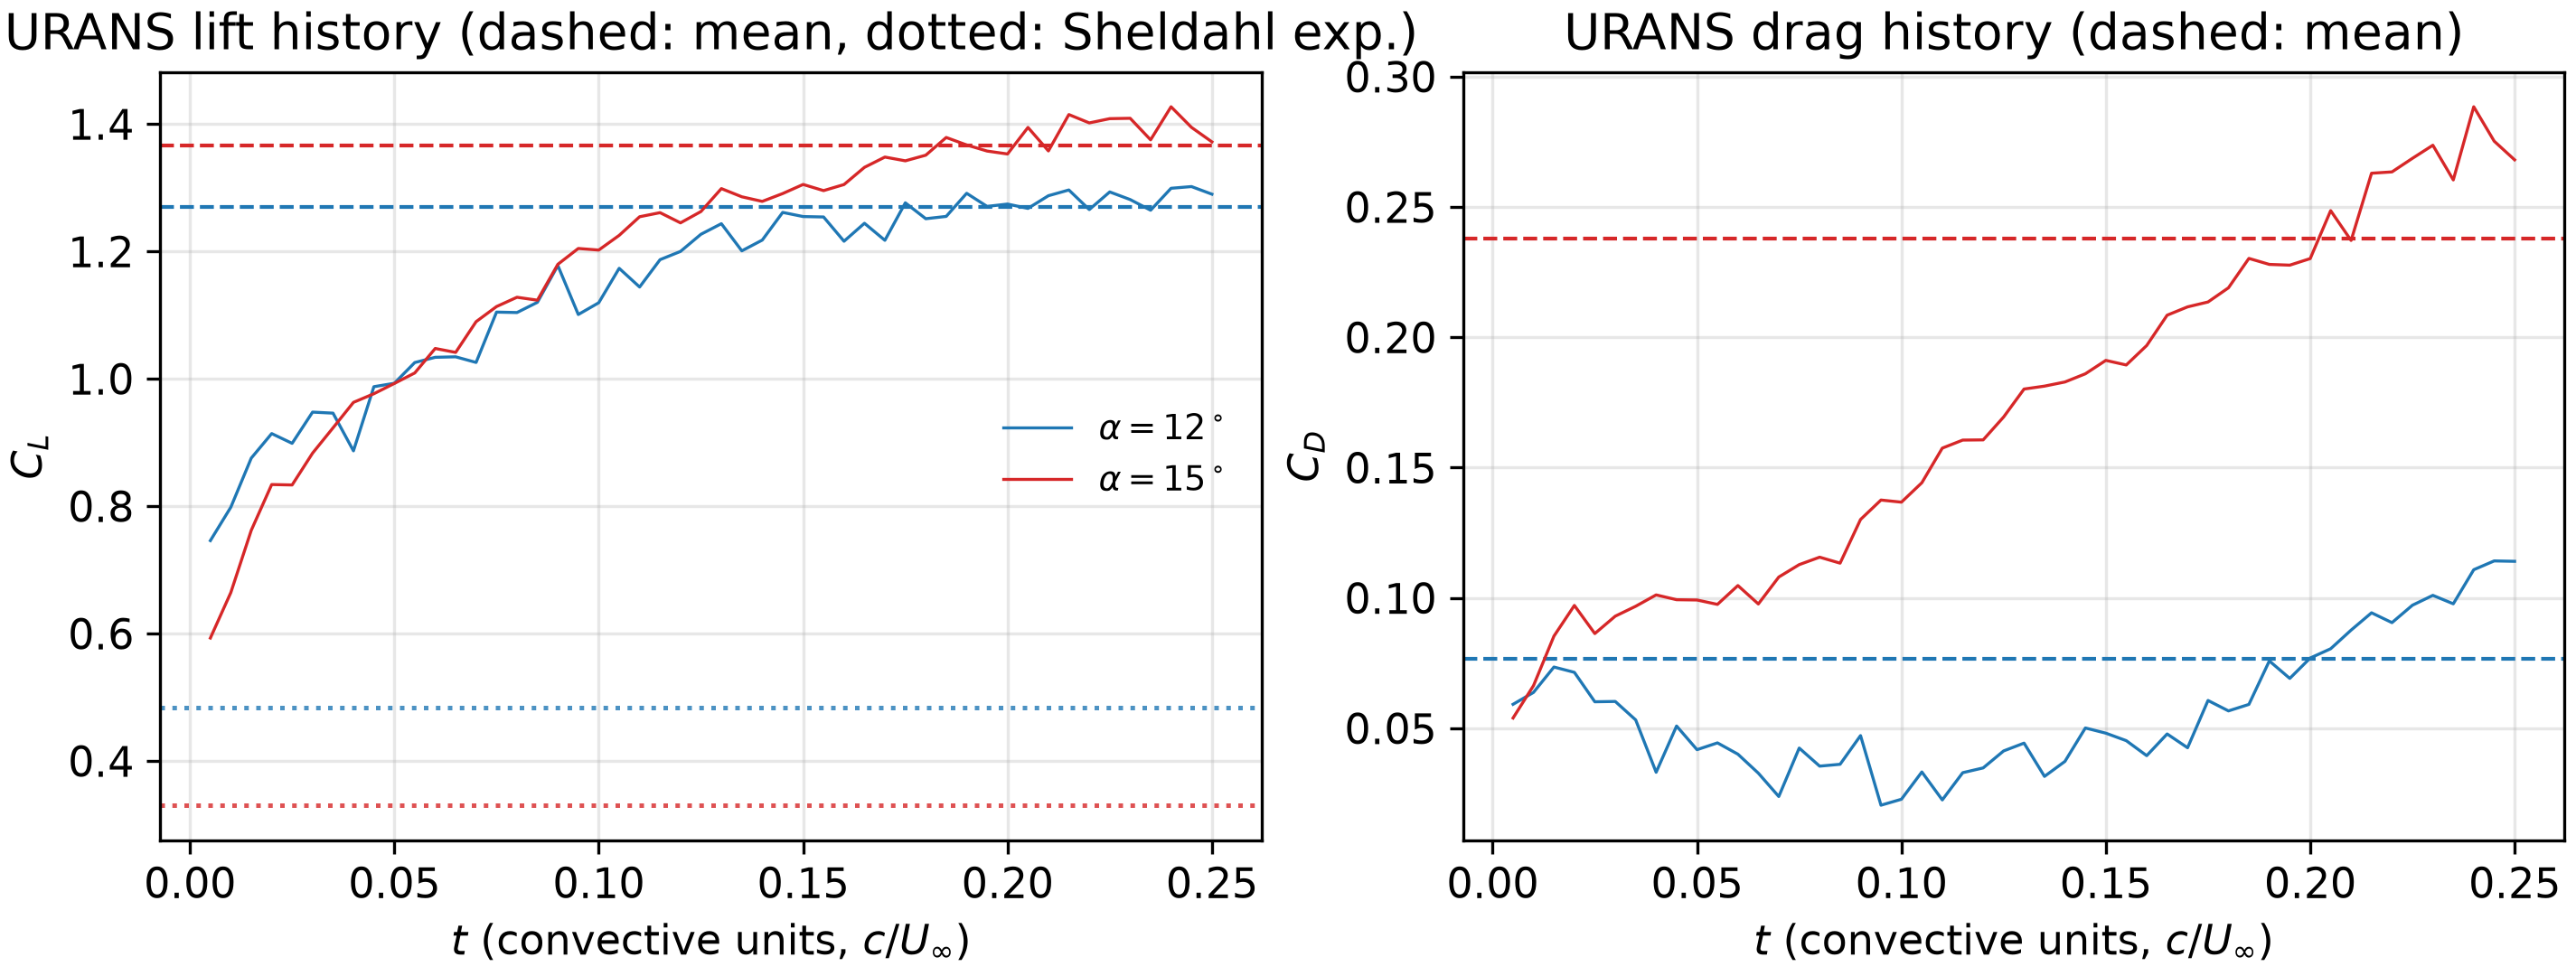
\includegraphics[width=0.98\textwidth]{figures/fig15_urans_history.png}
  \caption{URANS force histories for the NACA 0012 at $Re = 3.6\times10^5$: lift (left) and drag (right) versus convective time. Dashed lines: production-window means ($t = 0.15$--$0.25$); dotted lines: Reynolds-matched Sheldahl \& Klimas experimental values.}
  \label{fig:urans}
\end{figure}

\section{Discussion}\label{sec:discussion}

\subsection{Effect of camber}
Camber acts primarily through the zero-lift angle: all three sections carry the same attached-flow lift slope, but the cambered sections reach their operating lift at lower angles of attack and therefore retain a margin against the leading-edge pressure gradients that trigger stall. The maximum-lift ordering $4412 > 2412 > 0012$ and the efficiency peak shifting to higher $\alpha$ with camber are both consistent with the classical Abbott \& von Doenhoff compilations~\cite{abbott1959}.

The drag polars reveal a second, less obvious effect: the drag bucket of the cambered sections is displaced to non-zero lift, so at the operating lift coefficients relevant to small aircraft ($C_L \approx 0.4$--$0.8$) the NACA 2412 carries less drag than the 0012 would at the same $C_L$, while the 4412 begins to pay a growing profile-drag penalty from its stronger aft pressure recovery. In design terms, the cambered sections buy lift at fixed incidence but eventually pay for it in pressure drag; the efficiency curves (Figure~\ref{fig:eff}) show the trade quantitatively, with the 4412 peaking at the highest $C_L/C_D$ but over a narrower usable range.

\subsection{Stall mechanism in steady RANS}
In the present fully turbulent simulations, stall is always preceded by the same sequence: growth of the adverse gradient behind the suction peak, upstream migration of the $C_f = 0$ crossing, and finally large-scale separation covering the aft chord. Because the boundary layer is turbulent from the leading edge, no laminar separation bubble forms; the simulated stall is therefore the trailing-edge (mild) type for the cambered sections and turns leading-edge-like only in the deepest post-stall states. The steady solver reproduces the mean separated flow but cannot represent the unsteady vortex shedding that dominates real post-stall aerodynamics, which is visible physically as the slow force drift in the Appendix~B histories.

The absence of laminar-transitional physics deserves emphasis because it changes the \emph{character} of predicted stall at the lower end of the Reynolds range. In experiment at $Re = 10^5$, a laminar separation bubble typically forms near mid-chord, bursts near maximum lift, and produces an abrupt leading-edge-type stall; the fully turbulent model cannot generate a bubble, so it will instead predict a gradual trailing-edge stall. Users of the present results at $Re = 10^5$ should therefore read the computed lift and drag as the fully-turbulent envelope, not as a prediction of the transitional-flow aerodynamics that the experiments measure.

\subsection{Drag budget}\label{sec:dragbudget}
The computed drag at attached conditions exceeds the tripped experimental values by roughly $1.5$--$2\times$. Four contributors are identified: (i) the Reynolds gap --- the experiments are at $Re = 6\times10^6$ (Ladson, Abbott) or $2.88\times10^6$ (Gregory) against simulated $Re = 10^6$, and skin friction falls with $Re$, so a substantial share of the offset is a physical Reynolds effect rather than model error; (ii) the fully turbulent boundary layer lacks the long laminar run of the (even tripped) experiments, and turbulent skin friction is inherently higher; (iii) the open trailing edge produces a small base-drag penalty; and (iv) the trailing-edge seam cells of the polar topology locally degrade resolution. This is why the Reynolds-matched Sandia comparison (Section~\ref{sec:sandia}), which removes contributor (i) and replaces (ii) with the $\gamma$--$Re_{\theta t}$ closure, cuts the pre-stall drag MAE from $0.0102$ (fully turbulent) to $0.0068$. The lift, which is dominated by the pressure field, is much less affected --- hence the excellent lift agreement and the systematic drag offset. For design studies in which the drag \emph{difference} between configurations is the quantity of interest, this offset largely cancels.

This bias is not a defect of the SST model per se: the same fully turbulent setup on the TMR grids reproduces the CFL3D SST drag within a few percent, confirming that the offset is attributable to the physical modelling assumptions (and, secondarily, to grid resolution), not to solver error. Separating modelling error from discretisation error in this way is precisely why the code-verification step adds value beyond the experimental comparison.

\section{Limitations}\label{sec:limitations}
The interpretation of the present results is bounded by five modelling choices.

\textbf{Two-dimensionality.} Real airfoils at high lift exhibit three-dimensional separation cells and spanwise pressure gradients that alter stall behaviour; 2D RANS typically overpredicts $C_{L,\max}$ at low $Re$ and misplaces the stall angle. The experimental data near stall are themselves not strictly two-dimensional, as the TMR documentation notes for the NACA 0012 case: above $\alpha \approx 15^\circ$ the wind-tunnel measurements carry increasing three-dimensionality, which is one reason the datasets diverge there (Figure~\ref{fig:validation}).

\textbf{Steady RANS and partially unsteady verification.} Post-stall flow is inherently unsteady --- vortex shedding at a Strouhal number of order 0.2 based on the projected thickness dominates the loads. The steady solver converges to (at best) a mean flow, force oscillations are unrepresented, and the slowly drifting post-stall force histories (Appendix~B) indicate that the true mean flow may differ from the computed steady state by several percent in drag. The URANS subset of Section~\ref{sec:urans} verifies the near-stall regime in time-accurate mode, but at $\mathrm{Co} \le 20$ with a two-equation RANS closure it resolves shedding-scale dynamics only qualitatively; LES or resolved-transition simulation (e.g.\ $\gamma$--$Re_{\theta t}$--LES hybrids) remains out of scope.

\textbf{Partially resolved transition physics.} At $Re \le 10^6$ a significant fraction of the chord is laminar in experiment; the fully turbulent treatment inflates skin friction (the dominant cause of the drag offset quantified in Section~\ref{sec:dragbudget}) and suppresses the laminar separation bubble that governs low-Reynolds-number stall. The $\gamma$--$Re_{\theta t}$ repeats of Section~\ref{sec:transition} address this for the full low-$Re$ factorial and are validated against free-transition experiment at $Re = 3.6\times10^5$ (Section~\ref{sec:sandia}): attached-range drag error falls by one third, but the bubble-burst stall of the experiment is not reproduced by either closure, so the modelled low-$Re$ stall angle is an upper bound and quantitative bubble-driven stall prediction would require unsteady simulation with resolved transition dynamics.

\textbf{2D surrogates of 3D devices.} Serrations and tubercles operate through spanwise mechanisms that a strictly 2D model cannot represent: the sawtooth here acts only through its streamwise pressure-recovery signature, and the tubercle perturbation lacks the streamwise vortices that constitute its actual operating principle. Both device studies are accordingly reported only as a 2D negative control (Appendix~\ref{app:devices}); no conclusion about real device performance is drawn from them.

\section{Recommendations for future work}
Four extensions follow directly from the present findings. First, the URANS verification subset of Section~\ref{sec:urans} should be extended to the full low-$Re$ factorial (all three sections, both low Reynolds numbers, spanning the bubble-burst range) over horizons of $5$--$10$ convective units --- the present short-horizon window ($t = 0.25$, about $1.4$ flow passes) establishes the unsteadiness and the non-attractor finding but not fully stationary production-window statistics --- with grid refinement in the streamwise direction, and validated against the unsteady pressure signatures of the Sandia dataset. Second, a spanwise-periodic 3D domain (two to four tubercle wavelengths, periodic side boundaries) would allow the serration and tubercle mechanisms to operate as designed, at roughly two orders of magnitude higher cell count. Third, the low-$Re$ stall discrepancy exposed by the Sandia validation (Section~\ref{sec:sandia}) --- bubble-burst stall missed by steady 2D RANS with correlation-based transition --- calls for scale-resolving simulation with resolved transition dynamics, and for validation against cambered-section low-$Re$ data (e.g.\ UIUC low-speed tests). Fourth, the high-lift discrepancy between the medium-grid steady solutions and both experiment and CFL3D should be closed by a properly convergent grid family (geometric refinement ratio, farfield beyond 100 chords or a point-vortex correction) and a wake-aligned C-topology that removes the polar O-grid's stagnation-region non-orthogonality, following the TMR numerical-analysis protocol.

\section{Data and software availability}
All simulation cases, meshes, scripts, reference data, figures, and the compiled report are contained in the project repository (\texttt{projects/AERO-BLS/}). The software stack is entirely open source: OpenFOAM v2412 (ESI), Gmsh v2.2 mesh format, Python 3 with NumPy/SciPy/Matplotlib/meshio, and Tectonic for \LaTeX{} compilation. The experimental reference datasets are U.S.\ Government works in the public domain, obtained through the NASA Turbulence Modeling Resource. Each figure and table regenerates from the scripts alone; Appendix~\ref{app:repro} lists the exact pipeline order.

\section{Conclusions}
\begin{enumerate}
  \item Turbulent boundary layer separation on the NACA 0012 develops by upstream migration of the $C_f=0$ point from the trailing edge; on the production grid the migration accelerates sharply above $\alpha = 10^\circ$, reaching $x/c \approx \SepAfifteen$ at $\alpha = 15^\circ$ with a five-fold drag increase. A fine-grid repeat at $\alpha = 15^\circ$ remains attached, so the modelled separation onset is grid-sensitive and lies between $12^\circ$ and $15^\circ$; the qualitative stall sequence is robust across both grids.
  \item The $k$--$\omega$ SST closure, on a polar O-grid with resolved sublayer, reproduces the pre-stall lift of the NACA 0012 within \ClMAEpct{}~\% (MAE) of tripped experiment and within \CflThreeDClPct{}~\% of NASA's CFL3D SST reference; drag is systematically overpredicted by a quantifiable, configuration-consistent bias.
  \item Camber raises maximum lift and delays the efficiency collapse ($C_{L,\max}$: $4412 > 2412 > 0012$); reducing $Re$ from $10^6$ to $10^5$ degrades both lift and drag at fixed incidence.
  \item As a 2D negative control (Appendix~\ref{app:devices}), the serrated-trailing-edge surrogate \emph{increases} attached-flow drag and the tubercle surrogate is penalised at every incidence --- the expected failure modes of dimensionality-mismatched device models. No claim about real (3D) device performance follows from these computations; their role is to quantify the screening error.
  \item The Reynolds-number effect, sampled factorially over all three sections ($Re = 10^5$--$10^6$), degrades the attached-range force balance modestly (lift $-6$ to $-9\%$ at $\alpha = 10^\circ$, ordered by camber) but dominates near stall: at $Re = 10^5$ all three sections are fully separated by $\alpha = 18^\circ$ and maximum lift falls by $30$--$45\%$, an effective stall-angle reduction that the fully turbulent closure does capture through the momentum reserve of the low-$Re$ boundary layer.
  \item Transition-sensitive repeats with the $\gamma$--$Re_{\theta t}$ closure on the full low-$Re$ factorial (45 identical-grid cases) show that the fully turbulent envelope overpredicts attached-range drag by $2$--$26\,\%$ (growing as $Re$ falls) while missing the laminar separation bubbles ($x/c = 0.06$--$0.75$) that the transition model produces; near stall the closures diverge strongly (lift $-32$ to $+30\,\%$) as bubble burst reshapes the separation, and at $Re = 10^6$ the two agree within a few percent --- delimiting precisely where the cheaper fully turbulent treatment is fit for purpose.
  \item Low-Reynolds-number validation against the free-transition Sandia data ($Re = 3.6\times10^5$) confirms the drag ranking --- the transition closure cuts the attached-range drag error by \SandiaCdErrDropPct{}~\% --- but exposes a hard limit: the measured lift curve terminates in a bubble-burst stall at $\alpha = 10^\circ$--$12^\circ$ that neither steady 2D closure reproduces, so modelled low-$Re$ stall angles are upper bounds. Attached-range drag and lift from the transition model are, however, quantitatively usable.
  \item A URANS verification subset (pimpleFoam, $\mathrm{Co} \le 20$, 50-chord farfield grid) at the matched Reynolds number resolves the near-stall unsteadiness that the steady solver averages away: the time-averaged loads exceed the steady solutions by $22$--$29\,\%$ with $2$--$3\,\%$ lift fluctuations, demonstrating that the converged steady state is not an attractor of the time-accurate system; at $\alpha = 15^\circ$ the URANS drag lands within $25\,\%$ of the Reynolds-matched experiment against a $61\,\%$ steady underprediction.
\end{enumerate}

\begin{thebibliography}{9}
\bibitem{abbott1959} I.~H. Abbott and A.~E. von Doenhoff, \emph{Theory of Wing Sections}, Dover, New York, 1959.
\bibitem{mccroskey1987} W.~J. McCroskey, ``A Critical Assessment of Wind Tunnel Results for the NACA 0012 Airfoil,'' NASA TM-100019, 1987.
\bibitem{ladson1988} C.~L. Ladson, ``Effects of Independent Variation of Mach and Reynolds Numbers on the Low-Speed Aerodynamic Characteristics of the NACA 0012 Airfoil Section,'' NASA TM-4074, 1988.
\bibitem{gregory1970} N. Gregory and C.~L. O'Reilly, ``Low-Speed Aerodynamic Characteristics of NACA 0012 Aerofoil Sections,'' NASA R\&M 3726, 1970.
\bibitem{tmr} NASA Langley Turbulence Modeling Resource, \url{https://tmbwg.github.io/turbmodels/} (2D NACA 0012 validation case).
\bibitem{cfl3dtmr} NASA TMR, ``2D NACA 0012: CFL3D SST results,'' \url{https://tmbwg.github.io/turbmodels/naca0012_val_sst.html}.
\bibitem{menter1994} F.~R. Menter, ``Two-Equation Eddy-Viscosity Turbulence Models for Engineering Applications,'' \emph{AIAA Journal}, 32(8):1598--1605, 1994.
\bibitem{menter2003} F.~R. Menter, M. Kuntz, and R. Langtry, ``Ten Years of Industrial Experience with the SST Turbulence Model,'' \emph{Turbulence, Heat and Mass Transfer 4}, 2003.
\bibitem{langtry2009} R.~B. Langtry and F.~R. Menter, ``Correlation-Based Transition Modeling for Unstructured Parallelized Computational Fluid Dynamics Codes,'' \emph{AIAA Journal}, 47(12):2894--2906, 2009.
\bibitem{sheldahl1981} R.~E. Sheldahl and P.~C. Klimas, ``Aerodynamic Characteristics of Seven Symmetrical Airfoil Sections Through 180-Degree Angle of Attack for Use in Aerodynamic Analysis of Vertical Axis Wind Turbines,'' Sandia National Laboratories Report SAND80-2114, 1981 (DOI: 10.2172/6548367).
\bibitem{howe1991} M.~S. Howe, ``Noise Produced by a Sawtooth Trailing Edge,'' \emph{Journal of the Acoustical Society of America}, 90(1):482--487, 1991.
\bibitem{hansen2016} K.~L. Hansen, R.~M. Kelso, and B.~B. Dally, ``Performance Variations of Leading Edge Tubercles for Distinct Airfoil Profiles,'' \emph{AIAA Journal}, 49(1):185--194, 2011.
\bibitem{miklosovic2004} D.~S. Miklosovic, M.~M. Murray, L.~E. Howle, and F.~E. Fish, ``Leading-Edge Tubercles Delay Stall on Humpback Whale \emph{Megaptera novaeangliae} Flippers,'' \emph{Physics of Fluids}, 16(5):L39--L42, 2004.
\bibitem{spalart2000} P.~R. Spalart, ``Strategies for Turbulence Modelling and Simulations,'' \emph{International Journal of Heat and Fluid Flow}, 21(3):252--263, 2000.
\bibitem{schlichting1979} H. Schlichting, \emph{Boundary-Layer Theory}, 7th ed., McGraw-Hill, New York, 1979.
\bibitem{crabtree1957} L.~F. Crabtree, ``Effects of Leading-Edge Separation on Thin Wings in Two-Dimensional Incompressible Flow,'' \emph{Journal of the Aeronautical Sciences}, 24(8):597--604, 1957.
\bibitem{stratford1959} B.~S. Stratford, ``The Prediction of Separation of the Turbulent Boundary Layer,'' \emph{Journal of Fluid Mechanics}, 5(1):1--16, 1959.
\end{thebibliography}

\appendix
\section{Grid independence study}\label{app:grid}
Table~\ref{tab:grid} in Section~\ref{sec:method} summarises the three-density study at $\alpha=5^\circ$. The medium-to-fine change in $C_L$ is \ClGridDelta{} and in $C_D$ is \CdGridDelta{}, supporting the medium grid as the production mesh. The residual non-orthogonality maximum of $82.7^\circ$ is localised in the trailing-edge seam and does not affect the force integrals at this level of convergence.

At high lift the grid sensitivity is larger than at $\alpha = 5^\circ$, as expected for a flow with an incipient separated region: the fine-grid repeat of the $\alpha = 10^\circ$ case and the $\alpha = 12^\circ$/$15^\circ$ fine-grid repeats (Table~\ref{tab:gridhigh}) quantify this. The trend indicates that the medium grid progressively over-separates the flow at high incidence --- mildly at $10^\circ$--$12^\circ$ and dramatically at $15^\circ$, where the fine grid remains attached while the medium grid separates over most of the chord --- so the high-$\alpha$ force coefficients of the core matrix should be read with the fine-grid values as the more accurate estimate, and the modelled separation onset bracketed between $12^\circ$ and $15^\circ$. The extended-iteration repeat on the medium grid additionally separates convergence error from discretisation error.

Because the three densities refine non-uniformly (ratios 1.5 and 1.33 in each direction), a formal Richardson extrapolation is not strictly applicable; instead, the observed medium-to-fine changes (\ClGridDelta{} in $C_L$, \CdGridDelta{} in $C_D$ at $\alpha = 5^\circ$) bound the discretisation contribution to the production results. The dominant numerical uncertainty in the study is therefore not the interior discretisation but the trailing-edge topology: the open trailing edge and its seam cells introduce a small, configuration-consistent base-drag component that affects all cases equally and is discussed in Section~\ref{sec:dragbudget}.

\begin{table}[h]
  \centering
  \caption{Verification repeats at high lift (NACA 0012, $Re = 10^6$); the first four rows vary grid, iteration horizon, and farfield extent at $\alpha = 10^\circ$, the last four contrast medium and fine grids at $\alpha = 12^\circ$ and $15^\circ$.}
  \label{tab:gridhigh}
  \begin{tabular}{llrr}
    \toprule
    Configuration & Iterations & $C_L$ & $C_D$ \\
    \midrule
    \GridHighRows
    \bottomrule
  \end{tabular}
\end{table}

The farfield repeat isolates the domain-size contribution: enlarging the farfield from $20c$ to $50c$ \emph{reduces} the computed lift by $2.7\%$, so the farfield constraint cannot explain the remaining lift deficit relative to experiment at high incidence. The deficit is attributable to the physical modelling chain --- fully turbulent boundary layers, a steady closure, and moderate chordwise resolution of the leading-edge suction peak --- and is quantified, bounded by the repeats above, and carried through the interpretation of the high-$\alpha$ results.

\section{Solver convergence histories}\label{app:conv}
Figure~\ref{fig:conv} shows representative convergence histories. Attached cases meet the residual targets; post-stall cases reach the iteration limit with slowly drifting forces and are tail-averaged as described in Section~\ref{sec:method}.

\begin{figure}[h]
  \centering
  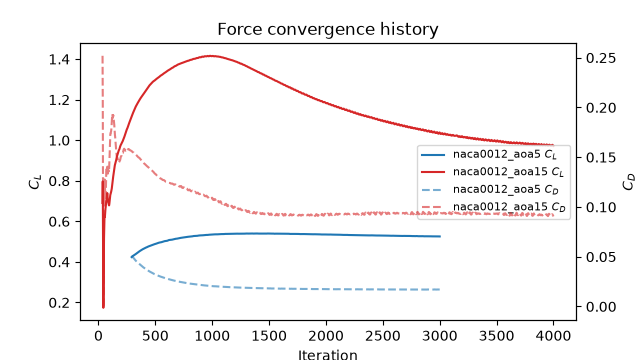
\includegraphics[width=0.75\textwidth]{figures/appendix_convergence.png}
  \caption{Force-coefficient convergence history, NACA 0012 at $\alpha=5^\circ$ and $\alpha=15^\circ$.}
  \label{fig:conv}
\end{figure}

\section{2D negative control for the passive devices}\label{app:devices}
The trailing-edge serration and leading-edge tubercle results are retained here as a \emph{negative control}, not as a device assessment. Both device classes derive their benefit from spanwise flow physics (pressure-equalising channels and streamwise-vortex generation respectively) that a 2D surrogate cannot represent; the value of the 2D computation is to quantify how badly a dimensionality-mismatched model fails, so that the main-text conclusion --- device effects are out of scope for 2D RANS --- is grounded in evidence rather than assertion.

\subsection{Passive drag reduction}

Table~\ref{tab:serr} compares the serrated trailing edge with the baseline NACA 0012, and the outcome is instructive precisely because it is negative at attached conditions: at $\alpha = 5^\circ$ the sawtooth \emph{increases} total drag by \SerrCdIncrFive{}~\% while costing \SerrClDropFive{}~\% lift, and at $\alpha = 10^\circ$ the drag penalty persists. Only in the deeply separated state ($\alpha = 15^\circ$) does the modification reduce drag (by \SerrCdDropFifteen{}~\%) while \emph{raising} lift by \SerrClRiseFifteen{}~\%, by partially re-energising the separated trailing-edge region and improving base-pressure recovery. The mechanism of the attached-flow penalty is visible in the geometry: the 2D sawtooth presents alternating notch faces to the streamwise pressure field, each acting as a small blunt base, and a strictly 2D model cannot produce the spanwise phase variation that makes real serrations benign or beneficial. The practical conclusions are that (i) the benefit of trailing-edge serrations is not accessible to a 2D surrogate at attached conditions --- a 2D sawtooth is a qualitatively different device, not a cheap approximation --- and (ii) in separated flow, geometric trailing-edge modification can still recover part of the base-pressure deficit. Both statements are consistent with the three-dimensional literature~\cite{howe1991,hansen2016} and quantify how much a 2D screening study can mislead if its surrogate geometry is interpreted literally.

The leading-edge tubercle is assessed with the same honesty, and the 2D surrogate verdict is harsher still. The surrogate here is a sinusoidal thickness modulation of the leading-edge region (amplitude $0.004c$, three waves over the front $30\%$ of chord, smoothly tapered to zero), which mimics the \emph{section-averaged} geometry change of a tubercled wing but not its spanwise mechanism: real tubercles act by generating counter-rotating streamwise vortices that keep attachment in the trough sectors, a topology a strictly 2D solution cannot contain. The result (Table~\ref{tab:tub}, Figure~\ref{fig:tubercle}) is a large penalty at every incidence: at $\alpha = 5^\circ$ the modulation \emph{increases} drag by \TubCdPctFive{}~\% while costing \TubClPctFive{}~\% of lift, at $\alpha = 10^\circ$ the drag penalty grows to \TubCdPctTen{}~\% with lift down \TubClPctTen{}~\%, and even in the deeply separated state ($\alpha = 15^\circ$) drag remains \TubCdPctFifteen{}~\% higher with \TubClPctFifteen{}~\% less lift. The skin-friction signature shows why: the wavy leading edge trips local separation immediately downstream of the leading edge --- at $\alpha = 10^\circ$ the upper-surface separation point sits at $x/c \approx 0.38$ on the tubercled section versus fully attached flow on the baseline --- and the separated patches over the modulation region destroy the leading-edge suction that the baseline exploits. Unlike the serrated trailing edge, which at least recovered base pressure once the flow was already separated, the 2D tubercle surrogate has no regime of benefit. This completes the passive-device study with a consistent message: \emph{both} leading- and trailing-edge passive devices derive their benefit from three-dimensional flow structures, and a strictly 2D surrogate of either class is not merely pessimistic --- it is a qualitatively different, and aerodynamically worse, device.

\begin{table}[t]
  \centering
  \caption{Trailing-edge serration effect, NACA 0012, $Re=10^6$ (2D sawtooth surrogate).}
  \label{tab:serr}
  \begin{tabular}{rrrrr}
    \toprule
    $\alpha$ [deg] & $C_L$ (baseline) & $C_L$ (serrated) & $C_D$ (baseline) & $C_D$ (serrated) \\
    \midrule
    \SerrTableRows
    \bottomrule
  \end{tabular}
\end{table}

\begin{table}[t]
  \centering
  \caption{Leading-edge tubercle surrogate (2D), NACA 0012, $Re=10^6$: forces relative to the smooth baseline.}
  \label{tab:tub}
  \begin{tabular}{rrrrrrr}
    \toprule
    & \multicolumn{3}{c}{Lift} & \multicolumn{3}{c}{Drag} \\
    \cmidrule(lr){2-4} \cmidrule(lr){5-7}
    $\alpha$ [deg] & baseline & tubercle & $\Delta$ & baseline & tubercle & $\Delta$ \\
    \midrule
    \TubTableRows
    \bottomrule
  \end{tabular}
\end{table}

\begin{figure}[t]
  \centering
  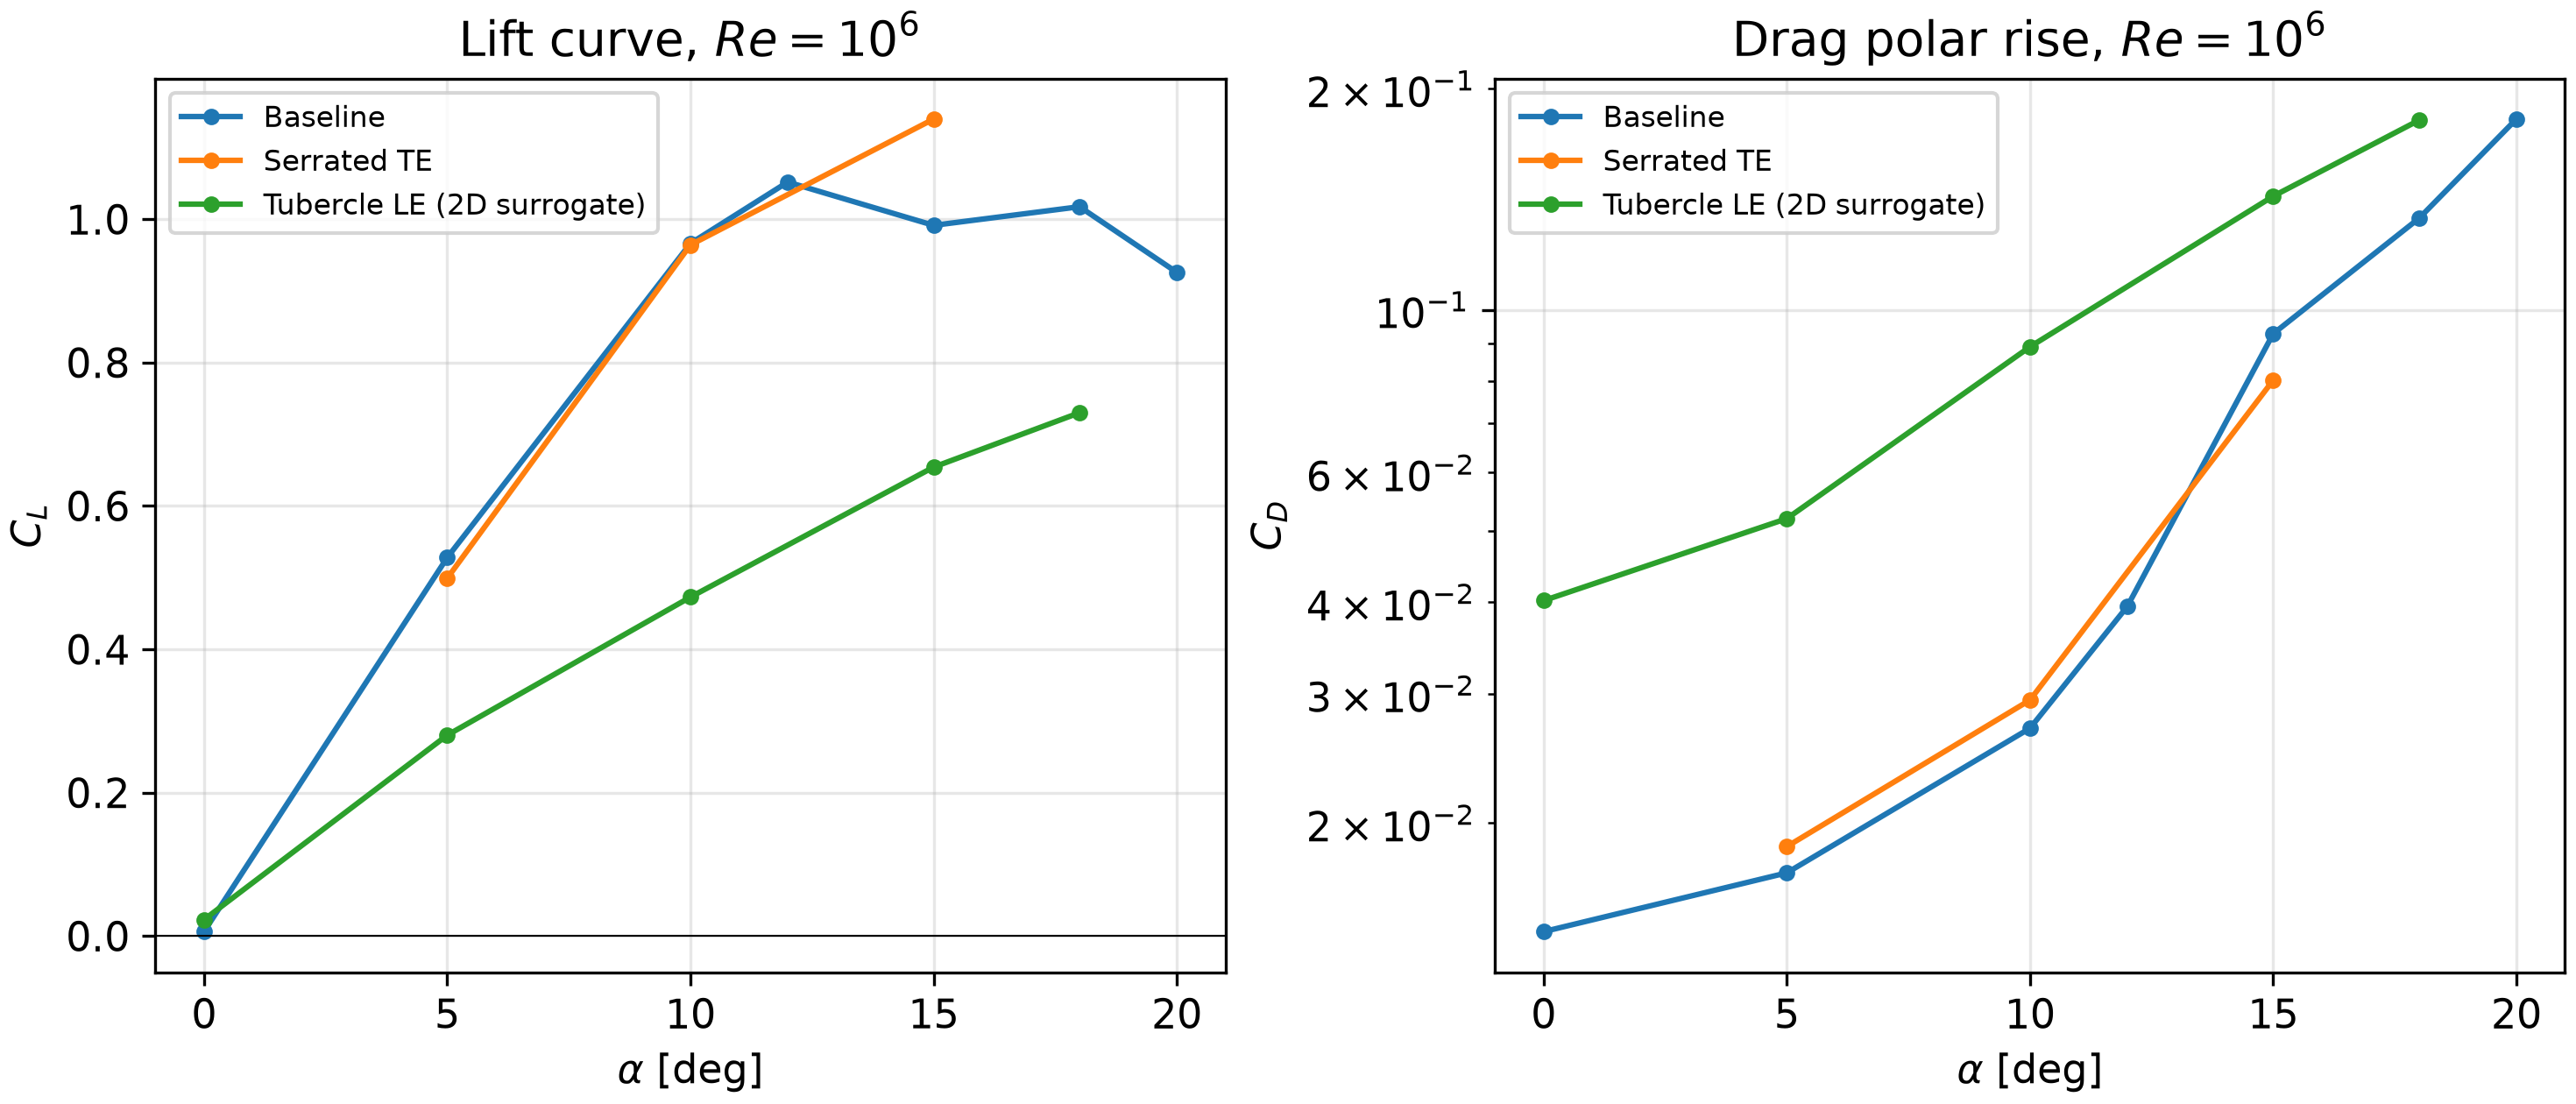
\includegraphics[width=0.92\textwidth]{figures/fig12_tubercle.png}
  \caption{Passive-device comparison on the NACA 0012 at $Re=10^6$: smooth baseline, serrated trailing edge, and leading-edge tubercle surrogate. Left: lift curves; right: drag (log scale).}
  \label{fig:tubercle}
\end{figure}

The skin-friction signature of the serrated configuration at $\alpha = 15^\circ$ (data archive) shows the mechanism directly: the reversed-flow region that covers the aft baseline chord is interrupted by short attached-flow strips on the tooth roots, restoring local $C_f > 0$ and with it a measure of pressure recovery. At $\alpha = 5^\circ$ the same notches introduce alternating acceleration/deceleration patterns on the otherwise smooth recovery, and the integrated effect is the observed drag increase. This contrast --- beneficial only once the baseline flow has already separated --- is the clearest single result of the drag-reduction study.



\subsection*{Implications of the negative control}
The serration results, read together with the separation map, support three practical statements. First, passive trailing-edge devices of this class operate on the pressure recovery, so they deliver their benefit only while the boundary layer is attached or mildly separated --- at $\alpha = 15^\circ$ in the present computations the serration is buried in a separated region and its effect reverses sign: drag drops by \SerrCdDropFifteen{}\% and lift rises. Second, at attached conditions the 2D sawtooth carries a drag \emph{penalty} of order \SerrCdIncrFive{}\%, so the net effect on $C_L/C_D$ must be evaluated for the actual operating condition; the surrogate device is not uniformly beneficial. Third, because the dominant benefit of real serrations and tubercles is three-dimensional (spanwise decorrelation, streamwise vortices), any design decision should be based on spanwise-periodic or full-3D simulations before hardware is committed; the present 2D workflow is the correct tool for screening the streamwise component and for building the separation map, not for final device design.

\section{Reproducibility manifest}\label{app:repro}
\enlargethispage{2\baselineskip}
Every number, figure, and table in this paper is produced by the pipeline in the project repository:
\texttt{01\_fetch\_airfoil\_coords.py} (geometry), \texttt{02\_generate\_mesh.py} (meshes),
\texttt{03\_prepare\_cases.py} (case staging), \texttt{04\_run\_all\_cases.sh} (batch execution),
\texttt{05\_postprocess.py} (forces, $C_p$, $C_f$, separation), \texttt{06\_generate\_figures.py}
(all figures), \texttt{07\_validate\_vs\_experiment.py} (validation tables), and
\texttt{08\_build\_report.py} (this document); a Bengali-language summary report is provided at \texttt{reports/report\_bn.md}. The experimental reference files in
\texttt{data/experimental/} are the TMR-distributed digitizations of the NACA datasets cited above.
Re-running the pipeline end-to-end regenerates every artifact from the scripts alone.

\end{document}
